\documentclass[11pt, a4paper]{report}
\usepackage{fontspec}
% FOR COLORFUL TABLES
\usepackage{booktabs}
\usepackage[table]{xcolor}
\usepackage[english]{babel}
%\usepackage[T1]{fontenc}
%\usepackage[utf8]{inputenc}
\usepackage{pdfpages}
\usepackage{array} % to make table column italic
\usepackage{textcomp} % to support the trademark symbol
%\usepackage[cache=false]{minted}
\usepackage{minted}

\usemintedstyle{autumn}
\usepackage{amsmath}
\DeclareMathOperator*{\argmax}{arg\!\max}
\DeclareMathOperator*{\argmin}{arg\!\min}
\usepackage[backend=bibtex,style=numeric,doi=false, url=false]{biblatex}  %backend=biber is 'better' 
\AtBeginBibliography{\small} 
%\bibliographystyle{unsrt_etal}
\addbibresource{bibliography.bib}
\usepackage{setspace}
\onehalfspacing

%\usepackage{unicode-math}
\usepackage{mathtools}
\usepackage{csquotes}
\DeclarePairedDelimiterX{\infdivx}[2]{(}{)}{%
  #1\;\delimsize\|\;#2%
}


\newcommand{\infdiv}{KL\infdivx}
\DeclarePairedDelimiter{\norm}{\lVert}{\rVert}

\newcommand\textfig[6][]{%
    % #1: content inside figure (optional)
    % #2: label
    % #3: alignment command
    % #4: width
    % #5: figure caption
    % #6: figure description
    \textfloat{#2}{#3}{\centering\includegraphics[width=#4]{#2}#1}{#5}{#6}}
   

\usepackage{subfiles}

%\setsansfont{Calibri}
\setmonofont{Ubuntu Mono}

%\setmonofont[Scale=MatchLowercase]{WenQuanYi Zen Hei Mon
%]{xits-math}

%\DeclareUnicodeCharacter{2010}{-}% support older LaTeX versions
\usepackage{wallpaper}
\usepackage{changepage}
\usepackage[version=4]{mhchem} % for isotope nomeclature support

% Setup captions
%\captionstyle[\centering]{\centering}
%\changecaptionwidth
%\captionwidth{0.8\linewidth}

% Protect against widows and orphanso}
%\setmathfont[
%    Extension=.otf,
%    BoldFont=*bold,
%\clubpenalty=10000
%\widowpenalty=10000

%\linespread{1.2}

%\raggedbottom

%\chapterstyle{ger}

%\maxsecnumdepth{subsection}

%%  Setup fancy style quotation
%%  ==================================================================
%\usepackage{tikz}
%\usepackage{framed}

%\newcommand*\quotefont{\fontfamily{fxl}} % selects Libertine for quote font

% Make commands for the quotes
%\newcommand*{\openquote}{\tikz[remember picture,overlay,xshift=-15pt,yshift=-10pt]
%     \node (OQ) {\quotefont\fontsize{60}{60}\selectfont``};\kern0pt}
%\newcommand*{\closequote}{\tikz[remember picture,overlay,xshift=15pt,yshift=5pt]
%     \node (CQ) {\quotefont\fontsize{60}{60}\selectfont''};}

% select a colour for the shading
%\definecolor{shadecolor}{rgb}{1,1,1}

% wrap everything in its own environment
%\newenvironment{shadequote}% 
%{\begin{snugshade}\begin{quote}\openquote}
%{\hfill\closequote\end{quote}\end{snugshade}}



%% MY STUFF


%% Language and font encodings

%% Sets page size and margins
%\usepackage[a4paper,top=2.5cm,bottom=2cm,left=2.5cm,right=2.5cm,marginparwidth=1.75cm]{geometry}
\usepackage{graphicx}
\usepackage{caption}
\usepackage{subcaption}
\captionsetup{font={small},skip=0.25\baselineskip}
\captionsetup[subfigure]{font={bf, footnotesize}, skip=1pt, singlelinecheck=false}
\graphicspath{{./plots/}{./figures/}}
\usepackage{subcaption}
\usepackage{float} % force float
\usepackage[nottoc]{tocbibind}

\usepackage[colorlinks=false, hidelinks]{hyperref}
\usepackage{cleveref} % for enumerate/itemize item referencing
\usepackage{parskip}% http://ctan.org/pkg/parskip
\usepackage{xspace}
\usepackage{wrapfig}
\usepackage[export]{adjustbox}
\usepackage{textcomp}
\usepackage[bottom]{footmisc}


\usepackage{titling}
\newcommand{\subtitle}[1]{%
  \posttitle{%
    \par\end{center}
    \begin{center}\large#1\end{center}
    \vskip0.5em}%
}

\renewcommand\thesubfigure{\arabic{subfigure}}  
\captionsetup{format=hang,labelsep=space,indention=-2cm,labelfont=bf,width=.9\textwidth,skip=.5\baselineskip}
%\captionsetup[sub]{labelfont=bf, labelsep=period,labelformat=simple, subrefformat=brace}


\usepackage{listings}
\lstset{basicstyle=\ttfamily,
  showstringspaces=false,
  commentstyle=\color{red},
  keywordstyle=\color{blue}
}

\makeatletter
\renewcommand\p@subfigure{\thefigure\,}
\renewcommand\thesubfigure{\alph{subfigure})}
% If desired for table as well:
% \renewcommand\p@subtable{\thetable\,}
% \renewcommand\thesubtable{\alph{subtable})}
\DeclareCaptionLabelFormat{mysublabelfmt}{\alph{sub\@captype}}
\makeatother

\renewcommand{\baselinestretch}{1.5}
\DeclareCaptionSubType*[arabic]{figure}



%\makeatletter
%\renewcommand\thesection{}
%\renewcommand\thesubsection{\@arabic\c@subsection}
%\makeatother

\usepackage{mathtools}
%\DeclarePairedDelimiter\abs{\lvert}{\rvert}%
%\DeclarePairedDelimiter\norm{\lVert}{\rVert}%

% Swap the definition of \abs* and \norm*, so that \abs
% and \norm resizes the size of the brackets, and the 
% starred version does not.
\makeatletter
\let\oldabs\abs
\def\abs{\@ifstar{\oldabs}{\oldabs*}}
%
\let\oldnorm\norm
\def\norm{\@ifstar{\oldnorm}{\oldnorm*}}
\makeatother



\usepackage{setspace}
\doublespacing 

\usepackage{etoolbox}
\makeatletter
\patchcmd{\@makechapterhead}{50\p@}{0pt}{}{}
\patchcmd{\@makeschapterhead}{50\p@}{0pt}{}{}
\makeatother



\usepackage{acro}
\acsetup{first-style=short}
\DeclareAcronym{MS}{
  short = MS ,
  long  = Mass Spectrometry,
  class = abbrev
}

\DeclareAcronym{MS1}{
  short = MS1 ,
  long  = first tandem MS analyzer ,
  class = abbrev
}



\DeclareAcronym{ROPE}{
  short = ROPE ,
  long  = Region Of Practical Equivalence,
  class = abbrev
}


\DeclareAcronym{IID}{
  short = IID,
  long  = Independent Identically Distributed,
  class = abbrev
}

\DeclareAcronym{MS2}{
  short = MS2 ,
  long  = second tandem MS analyzer ,
  class = abbrev
}

\DeclareAcronym{PSM}{
  short = PSM ,
  long  = Peptide-to-Spectrum Match(ing),
  class = abbrev
}


\DeclareAcronym{HGNC}{
  short = HGNC ,
  long  = Hugo Gene Nomenclature Committee,
  class = abbrev
}

\DeclareAcronym{MS/MS}{
  short = MS/MS ,
  long  = Tandem mass spectrometry,
  class = abbrev
}

\DeclareAcronym{MNAR}{
  short = MNAR ,
  long  = Missing Not At Random,
  class = abbrev
}



\DeclareAcronym{DAP}{
  short = DAP ,
  long  = Differentially Abundant Protein,
  class = abbrev
}


\DeclareAcronym{LOD}{
  short = LOD ,
  long  = Limit Of Detection,
  class = abbrev
}


\DeclareAcronym{KL}{
  short = KL ,
  long  = Kullback-Leibler (divergence),
  class = abbrev
}

\DeclareAcronym{ELBO}{
  short = ELBO,
  long  = Evidence Lower Bound,
  class = abbrev
}



\DeclareAcronym{m/z}{
  short = m/z ,
  long  = mass charge ratio,
  class = abbrev
}

\DeclareAcronym{MALDI}{
  short = MALDI ,
  long  = Matrix-Assisted Laser-Desorption Ionization,
  class = abbrev
}

\DeclareAcronym{ESI}{
  short = ESI ,
  long  = Electrospray Ionization,
  class = abbrev
}

\DeclareAcronym{GSEA}{
  short = GSEA,
  long = Gene Set Enrichment Analysis,
  class = abbrev
}


\DeclareAcronym{TOF}{
  short = TOF ,
  long  = Time of Flight,
  class = abbrev
}

\DeclareAcronym{IT}{
  short = IT ,
  long  = Ion Trap,
  class = abbrev
}

\DeclareAcronym{Q}{
  short = Q,
  long  = Quadrupole,
  class = abbrev
}

\DeclareAcronym{FT-ICR}{
  short = FT-ICR ,
  long  = Fourier Transform Ion Cyclotron Resonance,
  class = abbrev
}

\DeclareAcronym{HPDI}{
  short = HPDI,
  long  = High Probability Density Interval,
  class = abbrev
}

\DeclareAcronym{HPLC}{
  short = HPLC ,
  long  = High Pressure Liquid Chromatography,
  class = abbrev
}


\DeclareAcronym{MCMC}{
  short = MCMC,
  long  = Markov Chain Monte Carlo,
  class = abbrev
}


\DeclareAcronym{PTM}{
  short = PTM ,
  long  = Post-Translational Modification,
  class = abbrev
}

\DeclareAcronym{DAG}{
  short = DAG ,
  long  = Directed Acyclic Graph,
  class = abbrev
}


\DeclareAcronym{NZ}{
  short = NZ ,
  long  = Novozymes A/S,
  class = abbrev
}

\DeclareAcronym{FDR}{
  short = FDR ,
  long  = False Discovery Rate,
  class = abbrev
}

\DeclareAcronym{RT}{
  short = RT,
  long  = Retention time,
  class = abbrev
}

\DeclareAcronym{log2FC}{
  short = log2FC ,
  long  = $\log_2$(Fold Change),
  class = abbrev
}


\DeclareAcronym{MBR}{
  short = MBR ,
  long  = Match Between Runs,
  class = abbrev
}

\DeclareAcronym{VI}{
  short = VI ,
  long  = Variational Inference,
  class = abbrev
}

\DeclareAcronym{NUTS}{
  short = NUTS ,
  long  = No-U-Turn-Sampler,
  class = abbrev
}

\DeclareAcronym{MGF}{
  short = MGF ,
  long  = Mascot Generic Format,
  class = abbrev
}


\DeclareAcronym{XIC}{
  short = XIC ,
  long  = Extracted Ion Current,
  class = abbrev
}

\DeclareAcronym{SC}{
  short = SC ,
  long  = Spectral Counting,
  class = abbrev
}

\DeclareAcronym{TPP}{
  short = TPP ,
  long  = Trans Proteomic Pipeline,
  class = abbrev
}

\DeclareAcronym{NHST}{
  short = NHST ,
  long  = Null-Hypothesis Significance Testing,
  class = abbrev
}


\newcommand{\mycaption}[2]{\caption[#1]{\textbar\, \textbf{#1.} #2}}

%%  Begin document
%%  ==================================================================
	\begin{document}
%\singlespacing\blindtext

%%  Begin title page
%%  ==================================================================
    \thispagestyle{empty}
    \ULCornerWallPaper{1}{nat-farve.pdf}
    \ULCornerWallPaper{1}{nat-en.pdf}
    \begin{adjustwidth}{-3cm}{-1.5cm}
    \vspace*{-1cm}
    \textbf{\Huge Bioinformatics Master Thesis} \\
    \vspace*{2.5cm} \\
    \textbf{\Huge Development of label-free quantification \\ methods in proteomics} \\
    \vspace*{.1cm} \\
    %{\huge No subtitle is available} \\
    \begin{tabbing}
    % adjust the hspace below for the longest author name
    Antonio Ortega Jiménez \hspace{1cm} \= \texttt{<rnq313@alumni.ku.dk>}
    %Second Author \> \texttt{<second@author.com>} \\       
    \\[10.5cm] 
    
    \textbf{\Large Supervisors} \\
    Thomas Hamelryck \> \texttt{<thomas.hamelryck@gmail.com>} \\
    Mathias F. Gruber \> \texttt{<mafg@novozymes.com>} \\

    \end{tabbing}
    \end{adjustwidth}
    \ClearWallPaper
%%  ==================================================================
%%  End title page

%%%%%%%%%%%%% Indholdsfortegnelse %%%%%%%%%%%%%
\setcounter{tocdepth}{2}
\tableofcontents % Indholdsfortegnelse
\listoffigures   % Liste over figurer \begin{figure} ... \end{figure}
%%\listoftables    % Liste over tabeller \begin{table} ... \end{table}
%%%%%%%%%%%%%%%%%%%%%%%%%%%%%%%%%%%%%%%%%%%%%%%
\newpage

%\thispagestyle{empty}
%\printacronyms[include-classes=abbrev,name=Abbreviations]

\newpage
%\setcounter{page}{1}

% https://tex.stackexchange.com/questions/93859/condense-the-space-between-bibliographic-entries
\let\oldthebibliography\thebibliography
\let\endoldthebibliography\endthebibliography
\renewenvironment{thebibliography}[1]{
  \begin{oldthebibliography}{#1}
    \setlength{\itemsep}{0em}
    \setlength{\parskip}{0em}
}
{
  \end{oldthebibliography}
}

\section*{Preface}

TODO: get nomenclature straight: what is a sample and what is a fraction

\chapter*{Introduction}
\label{chap:introduction}

\section{Aminoacids and proteins}

Proteins represent the last link in the central dogma of biology, where information encoded in DNA, is transcribed to RNA for posterior translation into proteins at the ribosome.

Proteins are made up of 20 basic units, called aminoacids. All aminoacids share a common chemical structure, where a carbon atom ($C_\alpha$) is covalently bonded to a hydrogen atom, a carboxyl group, an amino group, and last but not least, a radical, also called side chain of the aminoacid. The side chain differs between aminaocids and generates them from each other. A slight deviation from this pattern exists in proline, where the radical is bound to the nitrogen atom, making it an iminoacid. Even though the side chains are all different, they can be classified into four different groups: aliphatic, polar, positively charged and negatively charged (see figure \ref{fig:aminoacids}).

%\textfig{aminoacids2.png}{body}{0.75\textwidth}
%    {The 20 aminoacids.}{CAPTION AND REFERENCE}
    
\begin{figure}
  \centering
  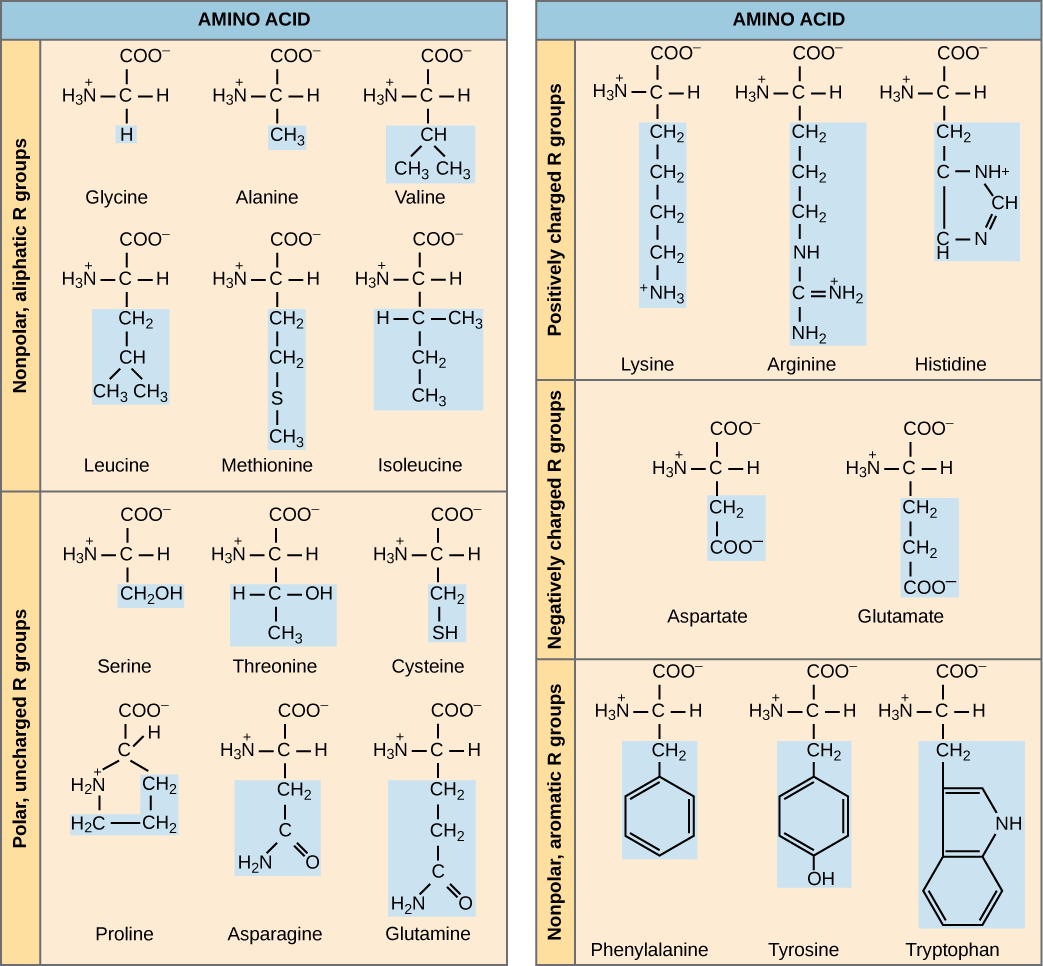
\includegraphics[width=0.8\textwidth]{aminoacids2.png}
  \caption[The 20 aminoacids]{CAPTION AND REFERENCE}
  \label{fig:aminoacids}
\end{figure}

Two aminoacids are joined together through the formation of a peptidic (covalent) bond between them. Such a linkage is formed by removal of the elements of water (dehydration) from the $\alpha$-carboxyl group of one amino acid and the $\alpha$-amino group of another \cite{Nelson2008}. The remaining $\alpha$-amino and $\alpha$-carboxyl groups are available for linkage to other aminoacids, and in this way peptidic chains or peptides can be created.

While there are 20 basic units that constitute the majority of naturally observable proteins, their side chains can be modified both by physiological processes and by experimental procedures cite. One frequent instance of such modifications is the oxidation of methionine.


\section{The protein-focused biotechnology industry}


Proteins carry out most of the cell\textquotesingle s molecular functions, they work as molecular agents that can perform an extremely wide range of tasks. The advent of biotechnology has sought to take advantage of this power, either by using proteins as present in natural conditions (wild type) or engineered by humans. This potential economic activity is carried out by several biotech companies, including Novozymes A/S (NZ).

\ac{NZ} is a company whose line of business consists of the development of enzymatic products performing chemical transformations in different industrial processes. The application of these products, instead of conventional chemical-based solutions, has the advantage that they require less chemical substances, potentially simplifying industrial processes, reducing their costs and their environmental impact. Notorious examples of such applications include waste-water treatment, household care and the baking industry.


The advancement of the way \ac{NZ} does protein research is thus key to place the organization ahead of its competitors. The refinement of the currently used tools and the development of new ones could be of great significance for the company. 

Protein research can be approached from different angles. This thesis exploited the combination of mass spectrometry (\ac{MS}) and proteomics workflows (see chapter \ref{chap:mass_spec}) for the qualitative and quantitative characterization of protein samples.



\section{Objectives of the Thesis}
\label{sec:objectives}

In line with the goal of making \ac{NZ} more competitive, this project aimed at the following objectives:

\begin{enumerate}

\item Develop an open-source, Linux based and easily deployable pipeline for the analysis of \ac{MS} data, starting at the raw high-throughput data files and ending in the  biological interpretation of the results.

\item Evaluate this pipeline with a benchmark dataset to assess if the pipeline is able to reflect the biological phenomena captured in the data.

\item Establish a label-free quantification probabilistic model that provides relative abundance estimates and a measurement of their uncertainty based on the available data.

\end{enumerate}

\section{Structure of the Thesis}

An overview over the \ac{MS} and following computational data analysis steps is presented in \ref{chap:mass_spec}. The pipeline development and its benchmark are explained in chapters \ref{chap:pipeline} and \ref{chap:benchmark}, while the modelling problem is introduced in chapter \ref{chap:model}. Finally, a conclusion of the work is given in chapter \ref{chap:conclusion}.
\chapter{Review on mass spectrometry (\ac{MS}) and shotgun proteomics}
\label{chap:mass_spec}


The main source of data in proteomics is \ac{MS}. However, different approaches to how this technique is used make for two paradigms in proteomics analysis: top-down and bottom-up \cite{Joshi2017}. In the top-down paradigm, intact proteins are directly used for the analysis \cite{Sinitcyn2018}. In the bottom-up paradigm (see figure \ref{fig:proteomics_overview}), the proteins are first cleaved into smaller parts, and these parts are then used for identification, characterization, and quantification. These smaller parts are peptides \cite{Barsnes2008}, consisting of around 10 chained aminoacids. Such peptides acquire physicochemical properties fitting the requirements of the downstream analytical methods, mainly the mass spectrometer (MS), which performs the data acquisition. The bottom-up paradigm is most often used because peptides are much more suitable to analysis by mass spectrometry, as illustrated in section \ref{subsec:the_detector}. This review will focus on the Data-Dependent Aquisition (\ac{DDA} approach within bottom-up proteomics, which currently is the most frequent workflow in proteomics \cite{Sinitcyn2018}. In this approach, the equipment is configured for the analysis of one peptide at a time, with the drawback of being biased for the most abundant peptides.

\begin{figure}[!h]
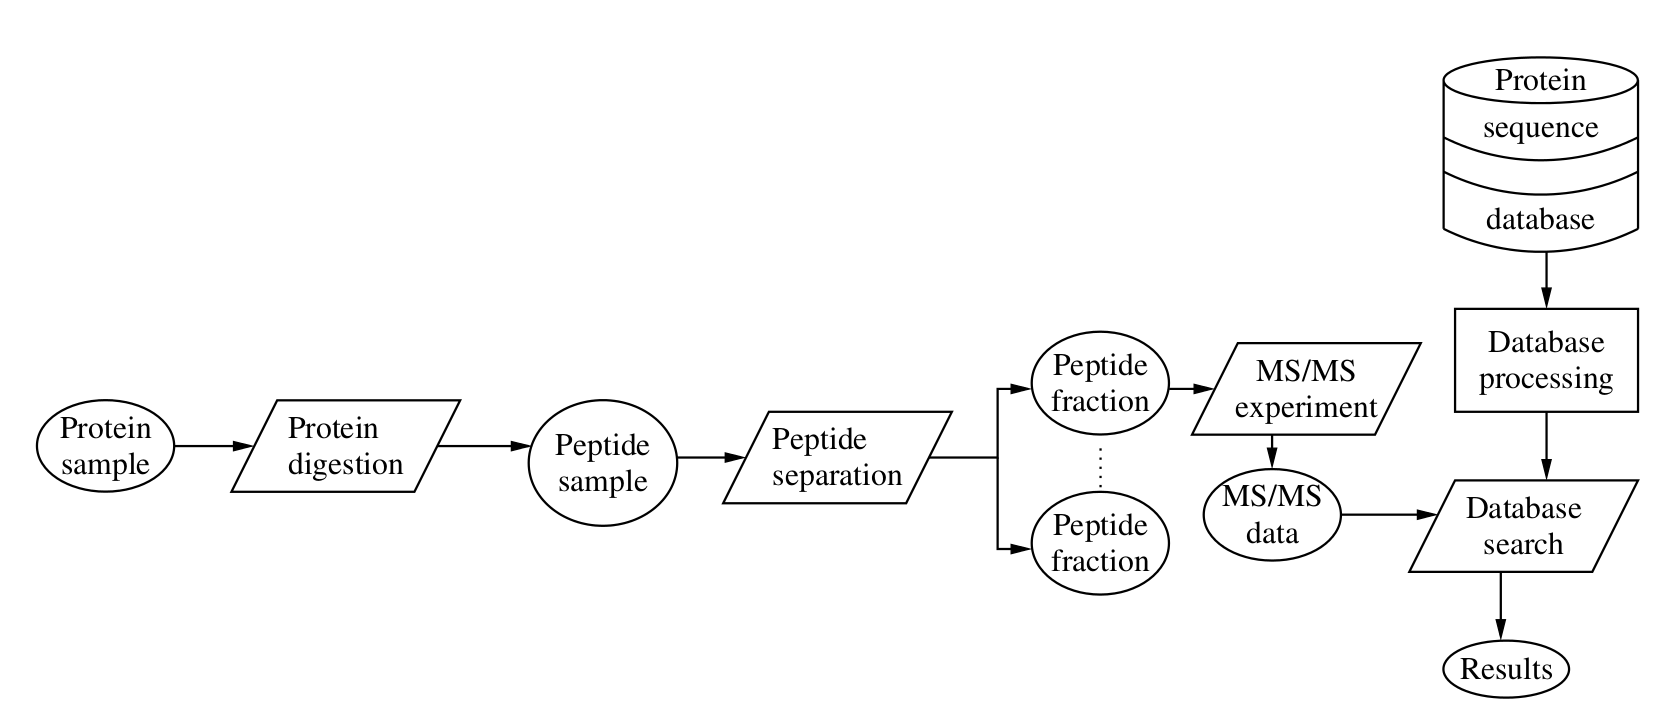
\includegraphics[width=\textwidth]{proteomics_skema_book}
\caption[Bottom-up proteomics analysis]{Diagram over a standard bottom-up proteomics analysis. Figure 1.3 from \cite{Barsnes2008}.}
\label{fig:proteomics_overview}
\end{figure}

MS is performed by means of a mass spectrometer, an ensemble of pieces of equipment that can acquire mass measurements for eventually thousands of sample components. A detailed explanation of the sample processing required prior to MS is given in section \ref{sec:sample_processing}, while an overview on mass spectrometers is given in section \ref{sec:the_mass_spectrometer}. The result of the MS analysis is a dataset that, with adequate computational analysis tools, is enough to perform the inference steps required to gather knowledge about the original protein sample. These inference steps can be condensed to the peptide and protein inference problems, explained in section \ref{sec:inference}. A third computational problem needs to be solved if quantitative, and not just qualitative information, is to be gained from the experiment. This is the quantification problem, explained in section \ref{sec:quantification}.

A summary of the bottom-up approach MS analytical pipeline is provided in the rest of the chapter. It can be divided into two main steps:

\begin{enumerate}

\item \ac{MS} analysis and data generation. Sections \ref{sec:sample_processing} to \ref{sec:tandem_ms_workflow}.

\item Computational analysis of data. Sections \ref{sec:search_engines} to \ref{sec:quantification}.

\end{enumerate}

\section{Sample processing}

Prior to its introduction in the mass spectrometer for shotgun proteomics studies, a protein sample (I) is cleaved into peptides and (II) these peptides are separated by means of some physicochemical properties. This way, the analytical equipment works with one peptide at a time.

\label{sec:sample_processing}

\begin{figure}[!h]
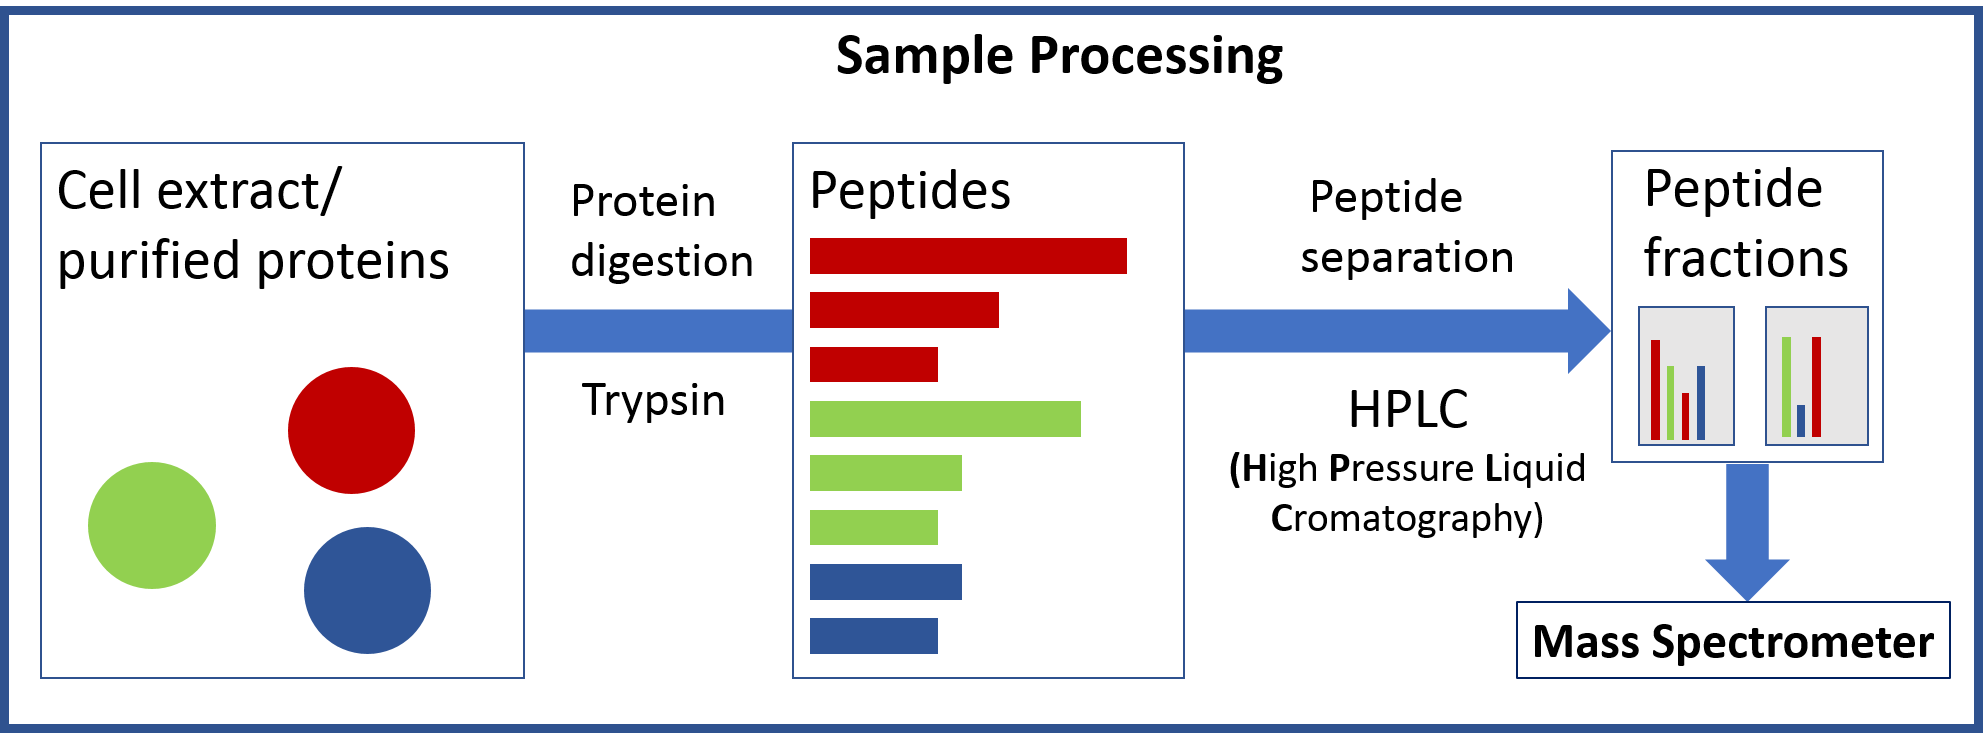
\includegraphics[width=\textwidth]{sample_processing}
\caption[Sample processing summary]{Diagram of the sample processing step prior to mass spectrometry analysis. First, proteins are denatured and digested with a specific protease like Trypsin. This yields a peptide mix that is separated into peptide fractions that can be introduced in the mass spectrometer.}
\label{fig:sample_processing}
\end{figure}

\subsection{Protein digestion}
\label{subsec:protein_digestion}

An \ac{MS} experiment starts with the generation of a protein sample from the biological system of interest. Proteins are then denaturalized  so as to remove bias due to the divergent properties acquired by folded proteins. Then, proteins are subjected to digestion with specific proteases i.e protein-cutting molecules, which cut the aminoacidic chains following a predictable pattern. Trypsin is the most frequently used protease. It cuts peptidic bonds whenever a positively charged residue, either Lysine (K) or Arginine (R), lies on the carboxyl side of the peptidic bond. Since roughly 1/10 residues are either R or K, the average peptide length is 10 residues, as mentioned before. As demonstrated in section \ref{subsec:the_detector}, this length distribution is fitted to the resolution of the MS analyzer. Moreover, in as much R and K are positively charged aminoacids (see figure \ref{fig:aminoacids}), the resulting peptide is guaranteed in most cases to be able to capture at least one charge, which is key in the \ac{MS} workflow as described in section \ref{sec:the_mass_spectrometer}. All of these properties combined, together with its low prize, makes Trypsin the protease of choice in this step for most cases.

Even though proteases are very specific, the cleaving process is far from perfect, as there could be: \cite{Barsnes2008}
%COMPUTATIONAL METHODS 3.2

\begin{enumerate}

\item Missed cleavages.

\item Unsuspected cleavages during the maturation/life cycle of the protein.

\item Unexpected cleavages occurring either in the wet-lab procedure of the proteolytic treatment.

\item Naturally occurring, intentionally or unintentionally induced chemical modifications.

\end{enumerate}

Missed cleavages can happen due to steric impediments or the presence of specific aminoacids that can weaken the enzyme\textquotesingle s function \cite{Siepen2007}. This is the case of Trypsin whenever the residue on the other side of the peptidic bond is Proline. Altogether, a variability is created in the cleavage process that, though limited, needs to be taken care of in downstream analysis, as it could introduce biases in peptide observability.

The result of this process is a complex mix of peptides, made up by hundreds or thousands of different molecules, following a length distribution given by the cleavage sites frequency and each protein\textquotesingle s aminoacidic composition. A peptide separation step is required before introducing the sample in the spectrometer.

\subsection{Peptide separation}
\label{subsec:peptide_separation}

If presented with the problem of analyzing a mixture of peptides, the capacities of mass spectrometers are easily overwhelmed by a too complex mixture, resulting in the analysis of only a minor part of the total protein of the sample \cite{Barsnes2008}. This can be surmounted by analyzing one peptide in the sample at a time. The required sample separation is achieved by High-Performance Liquid Cromatography (\ac{HPLC}) methods, like reverse phase chromatography (separating on hydrophobicity) and strong cation exchange chromatography (separating on isoelectric point) \cite{Barsnes2008}.

%CITE 4.2 computational methods.
During \ac{HPLC}, the peptide mix is loaded into a column containing a stationary and a solid phase. These phases create an environment where peptides interact differently based on their physico-chemical properties, set by the nature of the phases. The output of the column, called elute, will consist of subsets or fractions of peptides leaving the column at different retention times (\ac{RT}) i.e the amount of time passed before the peptide is observed in the mass spectrometer. Therefore, the input to the spectrometer will consist of few peptides at any given time.

\section{The mass spectrometer}
\label{sec:the_mass_spectrometer}

The mass spectrometer is the ensemble of pieces of equipment analyzing a peptide like as those generated following the workflow enunciated in sections \ref{sec:sample_processing} and \ref{subsec:peptide_separation}. It consists of three main parts: an ion source, a mass analyzer, and a detector (see figure \ref{fig:mass_spectrometer}) \cite{Barsnes2008}.

\begin{figure}[!h]
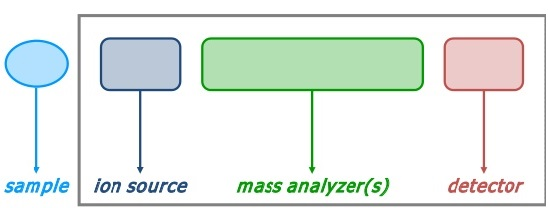
\includegraphics[width=\textwidth]{mass_spectrometer}
\caption[Mass spectrometer diagram]{Schematic view of a mass spectrometer. Taken from \footnotemark{}}
\label{fig:mass_spectrometer}
\end{figure}

\footnotetext{\href{https://www.slideshare.net/joachimjacob/bits-introduction-to-mass-spec-data-generation}{https://www.slideshare.net/joachimjacob/bits-introduction-to-mass-spec-data-generation}}
\stepcounter{footnote}

\subsection{The ion source}
\label{subsec:the_ion_source}

All mass spectrometers exploit the physical properties of mass and electric charge exhibited by the analyzed components. Ionization of the analytes is absolutely essential prior to any measurement, as analytes left uncharged will be unobservable to the equipment.

%CITE 5.1 COMPUTATIONAL METHODS

This step is performed in the ion source \cite{Barsnes2008}. The most frequent ionization methods in proteomics are Matrix-Assisted Laser Desorption-Ionization (\ac{MALDI}) and Electro Spray Ionization (\ac{ESI}) \cite{Mirzaei2016}. Most peptides ionized by MALDI will acquire a single charge, whereas ESI can provide multiple charges (+2, +3, etc) too \cite{Joshi2016}. Thus, the charge exhibited by an ion is not obvious when produced via ESI. Moreover, ESI can be run online with the right robotic equipment, while MALDI demands waiting time for vacuum generation. Finally, due to the chemical nature of the matrix components, MALDI ionizes more easily peptides containing aminoacids featuring aromatic rings (PYW) \cite{Hessling2013}, thus introducing a bias \cite{Hessling2013}. Bias in ESI is less predictable. All the sources of bias introduced during ionization cause the competitive ionization problem \cite{Zhang2009} \cite{Tang2004}.

The acquired charge yields a mass/charge (\ac{m/z}) ratio, a property that is applied in the downstream component separation and measurement steps. It is measured in $\frac{Da}{e}$, sometimes referred to as Th (Thomson).

\subsection{The mass analyzer}
\label{subsec:the_mass_analyzer}

The plethora of ion separation methods is reflected upon the range of different analyzers available, mainly time of flight (\ac{TOF}), Ion trap (\ac{IT}) and quadrupole (\ac{Q}). These apply different principles to perform the same task: separation (analysis) of the ion mix by the \ac{m/z} ratio.

Moreover, two other analyzers exist which combine mass analysis with intensity measurement. These are Fourier Transform Ion Cyclotron Resonance (\ac{FT-ICR}) and Orbitrap. They both register cylotron resonance frequencies that are Fourier transformed into the spectrum space. Remarkably, \ac{FT-ICR} exhibits great resolving power, at the cost of high maintenance costs and difficult operability \cite{Barsnes2008}. 

\subsection{The detector}
\label{subsec:the_detector}

Detectors measure the intensity of an incoming ion signal. The ion\textquotesingle s \ac{m/z} ratio is known thanks to the previous mass analysis step. Performed for enough \ac{m/z} ratios, the detector can produce a \ac{MS} spectrum, which shows the intensity of ion current over an \ac{m/z} range. Some topics in signal detection in \ac{MS} need to be discussed.

On the one hand, the precision of the signal measurement is given by its mass resolution It is conventionally defined as the closest distinguishable separation between two peaks of equal height and width \cite{Marshall2013}. The resolution decreases as the \ac{m/z} ratio increases because small increments in the \ac{m/z} ratio become negligible at high \ac{m/z} ratios. This is one of the reasons why proteins are better fit for analysis when digested into peptides, as \ac{m/z} are reduced, thus increasing the mass resolution.

On the other hand, due to the natural occurrence of isotopes, particularly \ce{^{13}_{}C}, the same peptide will induce the measurement of several signals with very close \ac{m/z} values. They constitute the isotopic envelope of the ion (see figure \ref{fig:envelope}) \cite{Mirzaei2016}, and represent the signal created by peptides containing an increasing number of \ce{^{13}_{}C} atoms or other naturally occurring isotopes. Every time a \ce{^{12}_{}C} is replaced by \ce{^{13}_{}C}, the mass increases by 1 Da. Even though the natural abundance of \ce{^{13}_{}C} is 1.1 \%, the sheer number of carbon atoms in a peptide makes it likely that at least one or even more carbon atoms will be \ce{^{13}_{}C}, eventually driving the pure \ce{^{12}_{}C} signal to comparatively small intensity values, and down to intensities below the background noise. Such event can be problematic if it entails that the \ce{^{13}_{}C} peak is confused for the \ce{^{12}_{}C} peak.

\begin{figure}[!h]
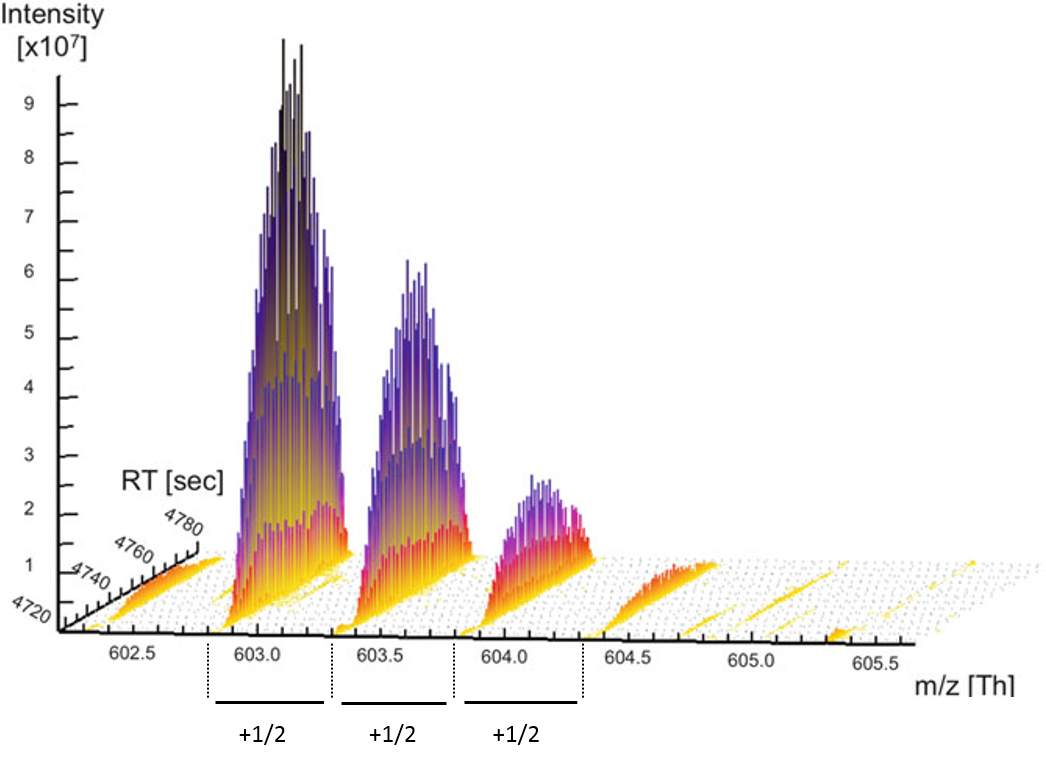
\includegraphics[width=\textwidth]{envelope}
\caption[Isotopic envelope]{A doubly charged isotopic envelope with its monoisotopic ion measured at 602.8 Th. Each peak in the envelope is separated by 0.5 Th. This is explained by the peptide having 2 positive charges that make every extra Da in the ion mass account for 1/2 extra Th. Adapted from \cite{Mirzaei2016}.}
\label{fig:envelope}
\end{figure}


The resolution achieved by modern equipment allows for the distinction of each individual signal in most isotopic envelopes. Remarkably, the separation across peaks in the envelope can be used to infer the charge of the peptide with the following expression.

\begin{equation}
m/z = \frac{(m + z × H^+)}{z} \text{for \textit{z}} \in {1, 2,...}
\end{equation}

where $H^+$ is the mass of a single charge (1 Da) and $z$ is the number of charges acquired. A single charge will induce a separation of 1 \ac{m/z}, while at charge 2 it will be $1/2 = 0.5$ \ac{m/z}, at 3 $1/3 = 0.33$ \ac{m/z}, and so on (see figure \ref{fig:envelope}).

It is up to the \ac{MS} technician to decide on the best pieces of equipment according to their availability and particularities of the dataset.

\section{Tandem MS workflow}
\label{sec:tandem_ms_workflow}

\begin{figure}[!h]
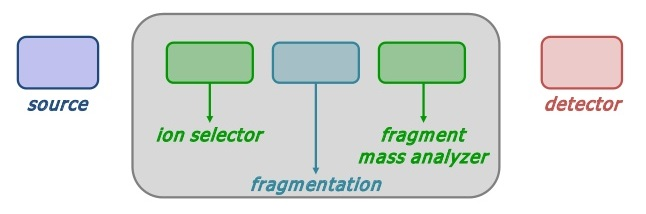
\includegraphics[width=\textwidth]{tandem_ms}
\caption[MS/MS schema]{Illustration of the tandem MS workflow. The first spectrometer acts as an ion selector, that not only registers spectra, but also lets through ions with a given \ac{m/z} ratio. The second spectrometer does not perform mass analysis, but instead provides the medium where peptide fragmentation (see section \ref{subsec:fragmentation}) occurs. Finally the third spectrometer records fragment mass spectra. Taken from \footnotemark{}.}
\label{fig:tandem_ms}
\end{figure}

\footnotetext{\href{https://www.slideshare.net/joachimjacob/bits-introduction-to-mass-spec-data-generation}{https://www.slideshare.net/joachimjacob/bits-introduction-to-mass-spec-data-generation}}
\stepcounter{footnote}

Shotgun proteomics analyses make use of two or more mass spectrometers connected in series, giving rise to the so-called Tandem MS (\ac{MS/MS}) workflow. In this setting, each mass spectrometer collects a different type of spectra and thus different information (see figure \ref{fig:shotgun}). An extra spectrometer, usually a quadrupole, is introduced in between.

\begin{itemize}

\item The first spectrometer records the intensity versus \ac{m/z} ratio of the peptides eluting from the column at a given time and is used to filter ions exhibiting a selected \ac{m/z} ratio (in the \ac{DDA} protocol).

\item The ions filtered in the first spectrometer undergo fragmentation in the second spectrometer. %, as explained in \ref{subsec:fragmentation}.

\item The last spectrometer records the intensity versus \ac{m/z} ratio of the fragments produced in the previous step. The resulting spectrum can be use to read out the peptide sequence.

\end{itemize}

\begin{figure}[!h]
\centering
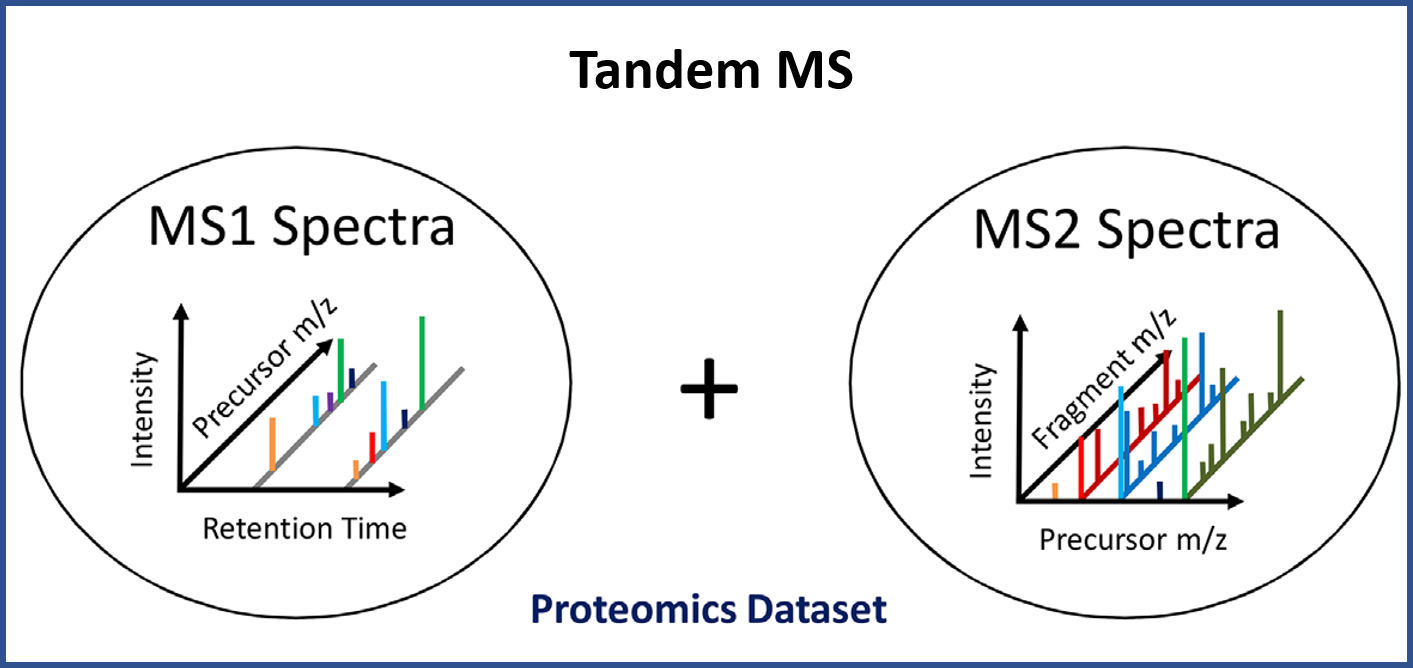
\includegraphics[width=\textwidth]{shotgun_adapted}
\caption[MS/MS spectra]{Illustration of the different spectra collected in tandem MS. MS1 spectra record precursor intensity vs \ac{m/z} ratio at different times. MS2 spectra record the same magnitudes but the signal is generated by the fragments produced during fragmentation by the ion filtered in the first spectrometer. Altogether, they enable peptide identifications. Figure adapted from \cite{Verheggen2017}.}
\label{fig:shotgun}
\end{figure}

\subsection{Fragmentation}
\label{subsec:fragmentation}

Fragmentation occurs in the second spectrometer. But what is it, and why is it done? The information that can be extracted from \ac{MS1} scans consists of the \ac{m/z} ratio and retention time of the peptide ion, but not its sequence. Having the latter is paramount if the spectrum is to be matched to a theoretical peptide. Fortunately, the peptide sequence of the ion can be inferred if fragmentation is performed.

\begin{figure}[!h]
\centering
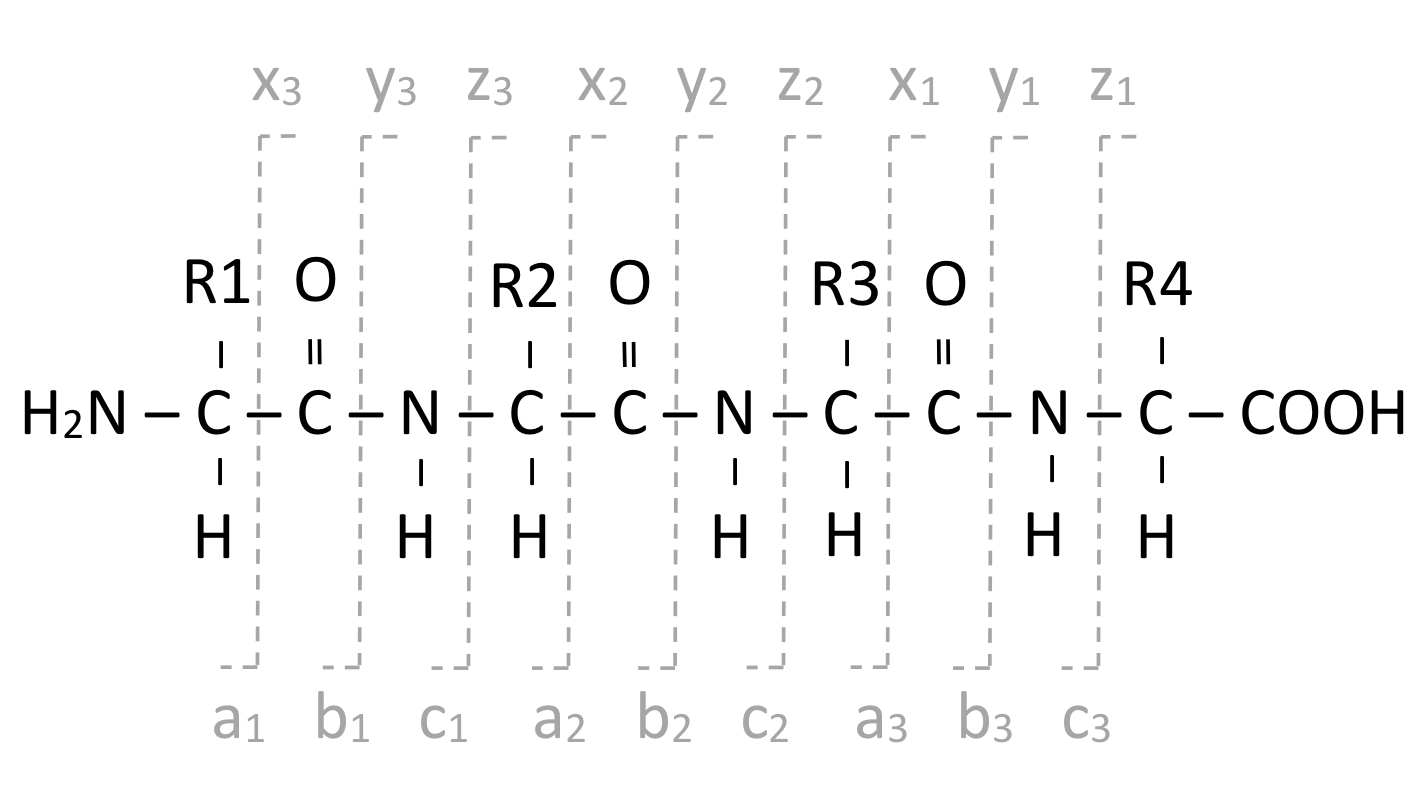
\includegraphics[width=0.8\textwidth]{abcxyz}
\caption[Fragment ions nomenclature]{The common fragments and their relation to the peptide sequence can be organized into 2 groups of 3 series each. The abc fragments keep the N-terminal residue, while xyz keep the C-terminal one. Specific fragmentation techniques make fragments belonging to one series more likely than others. Other fragments are possible but much less likely. The fragment nomenclature was introduced in \cite{Roepstorff1984}.}
\label{fig:abcxyz}
\end{figure}


During peptide fragmentation, bonds along the peptidic chain are broken, turning the peptide into smaller fragments. These fragments will consist of truncated versions of the original peptide at different positions, thus making it possible to read an \ac{m/z} ratio difference between any pair of fragment ions. The difference can be exploited to deduce which aminoacid makes up for that difference. If this process is repeated for enough pairs of contiguous fragments, with the right software, a sequence can be read from the \ac{MS/MS} spectrum, as  explained in section \ref{sec:search_engines}.

%A given bond will be more likely to break the less stable it is. This makes (I) the \ce{C_$\alpha$}-\ce{CO}, (II) the peptidic \ce{CO}-\ce{NH}, and (III) the \ce{C_$\alpha$}-\ce{NH} bonds the most likely to break (see figure \ref{fig:abcxyz}). A nomenclature REF was introduced to name these fragments:



%%PAG 123 COMPUTATIONAL METHODS
%Fragmentation in proteomics is performed via (I) collision-induced (CID) or (II) electron-induced (EID) dissociation. CID is an ergodic fragmentation technique where peptides enter a collision cell containing an inert gas. Given enough kinetic energy, hits between ionized peptides and the gas will trigger the fragmentation of the peptide into smaller units. \cite{Barsnes2008}. Since the kinetic energy is randomly distributed across the peptide, the weakest bonds will break first. This results in the production of mostly b and y fragments, as well as the loss of any chemical modifications \cite{Barsnes2008}.
%
%%CITE pag 134 computational methods
%
%EID is produced by the hits against the molecule, which tend to occur on the areas of the peptide more positively charged. Thus, the fragmentation process is not ergodic and returns TYPE ions. More importantly, chemical modifications are not lost in the process.
 
\section{Spectra processing: search engines}
\label{sec:search_engines}

Computational analysis of MS data starts with the matching of the spectra to a referene proteome (see figure \ref{fig:computational_analysis}). \ac{MS} search engines are capable of performing the crucial step of peptide to spectrum matching (PSM). During this step, search engines perform (I) \textit{in silico} prediction of the peptides produced in the protein digestion step and (II) their expected spectrum.


\begin{figure}[!h]
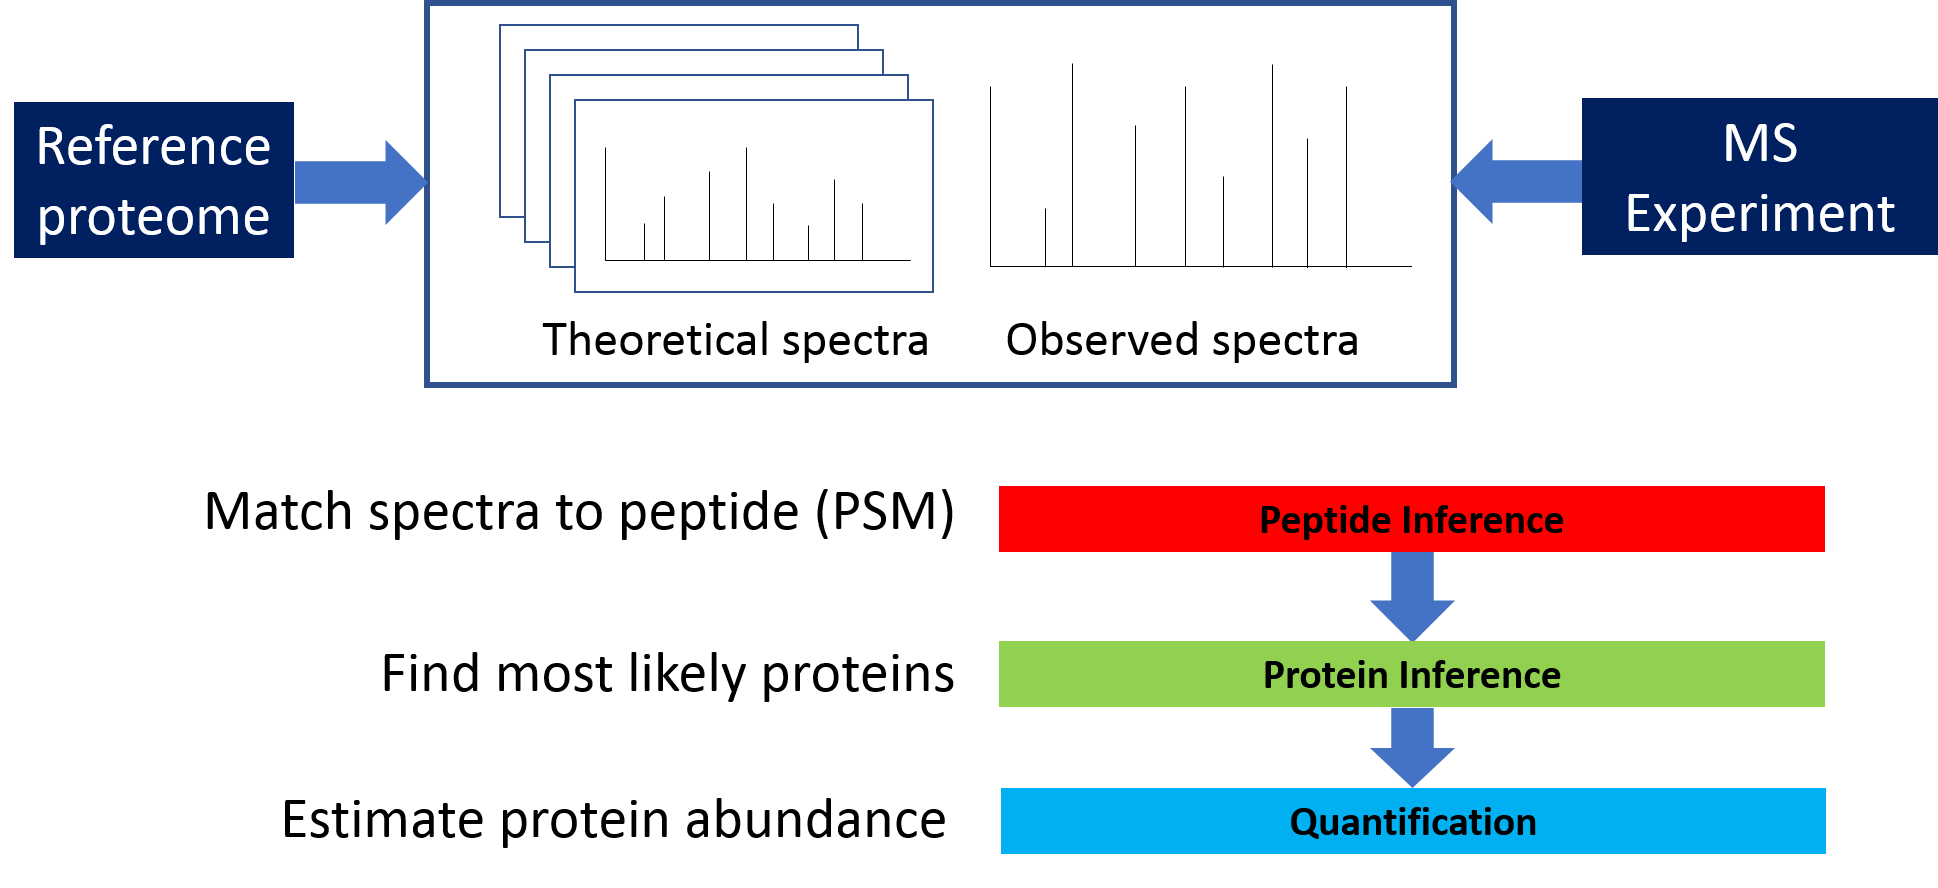
\includegraphics[width=\textwidth]{computational_analysis}
\caption[Mass spectrometry computational analysis]{Diagram of the MS computational analysis. The PSM process maps the observed spectra to a list of peptides in the reference proteome that could have generated them. In other words, the software infers what peptides were introduced in the spectrometer. The analysis continues during protein inference and quantification.}
\label{fig:computational_analysis}
\end{figure}

%\begin{figure}[!h]
%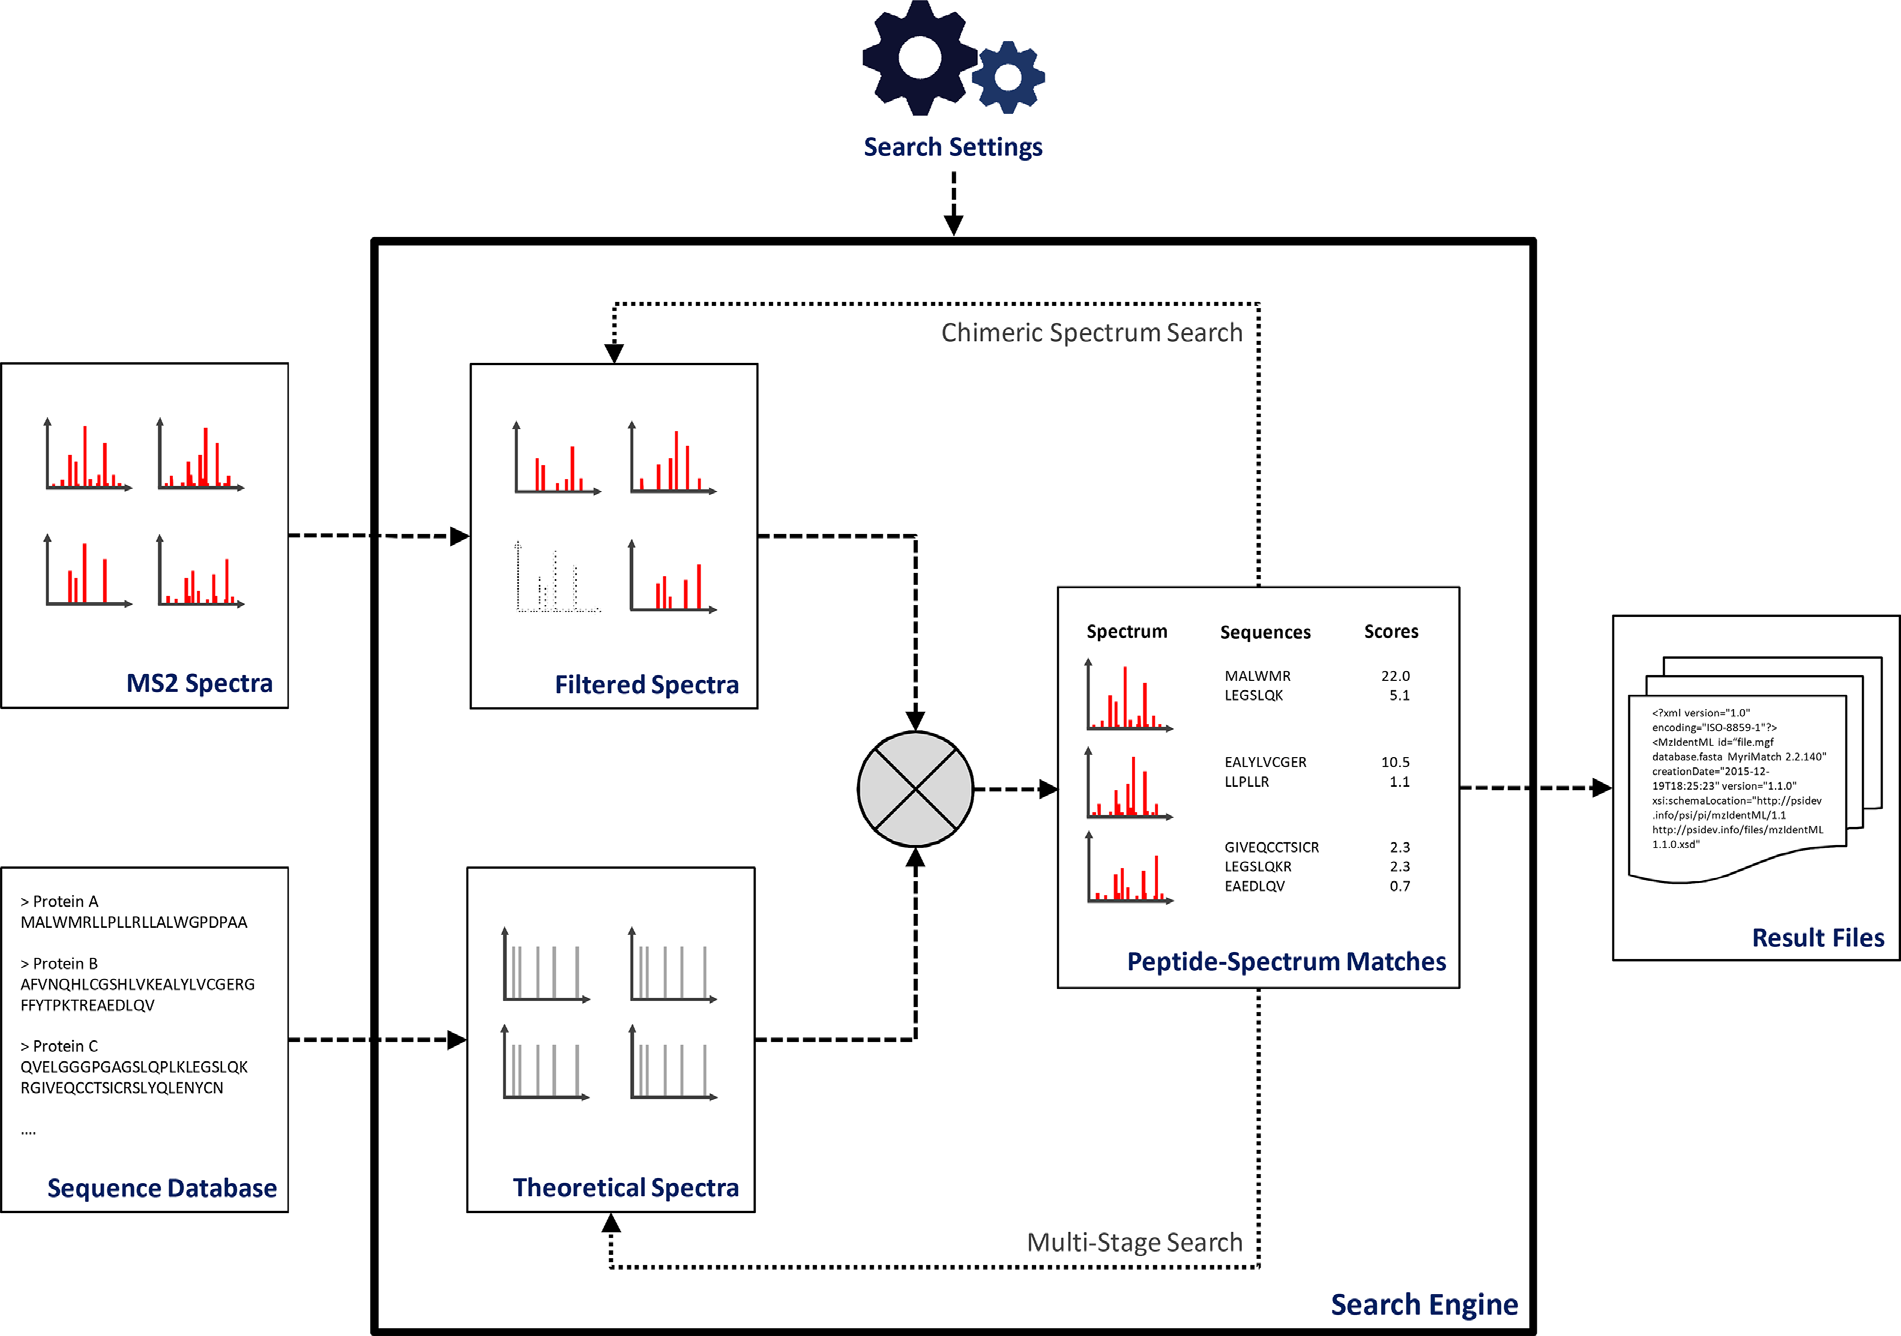
\includegraphics[width=\textwidth]{PSM}
%\caption{}
%\label{fig:PSM}
%\end{figure}

Given the stochastic nature of the protein cleavage and spectra recording processes, the resulting data exhibit variability manifested in both missing and spurious peaks \cite{Stein1999}. Furthermore, random (wrong) matches can be returned by the PSM process when running against a sufficiently big database. This translates to the generation of multiple matches, of which one, if any, will be correct. Therefore, the lists of matches need to be somehow ranked by goodness-of-fit. The issue is addressed by search engines through the deployment of statistical models that provide scoring systems. Assuming the correct protein is present in the database, a good scoring system should give the best score to the right peptide. Under this circumstances, if repeated for several peptides, enough evidence for the presence of individual proteins can be collected.

Multiple search engines exist that implement different matching and scoring algorithms. The most modern ones include MS-GF+ \cite{Kim2014}, MS-Amanda \cite{Dorfer2014}, Comet \cite{Eng2013} and Andromeda \cite{Cox2011}. Notably, the results of each individual search engine can be combined to gather their strengths, at the expense of an increased computational cost and time \cite{Shteynberg2013}.



\section{Validation and quality control}
\label{sec:validation}

The scoring systems implemented in search engines provide the best matches, but they are bound to contain false identifications. Nevertheless, these scores can be used to apply a filter that aims at minimizing the amount of errors.

A common filter is the false discovery rate (FDR), usually set to 1\%, indicating that after its application, only one out of a hundred filtered matches are expected to be false positives (wrong matches).

The most commonly used method to compute the \ac{FDR} of a list of matches is the target-decoy search. Using this method, the search engine replicates the matching process, using the same spectra, but instead against a decoy database i.e it simulates random matches. The decoy database is generated by reversing or more generally applying a randomization technique upon the sequences present in the original database (target) \cite{Elias2010}. 

All matches to the decoy are by definition wrong. Since the basic properties of the decoy (size, composition, etc) remain identical to those of the target the amount of matches to the decoy exhibiting more than a given score $s$ can be regarded as an estimate of the number of false identifications ($\hat{n}_{fp}$) in the list of target results exhibiting at least the same score. This is because the existence of shared properties entails that random matches are equally likely to happen in both databases \cite{Elias2010}. Together with the number of PSMs passing a given score in the target ($n_{tp} + n_{tp}$), the FDR can be computed using equation \ref{eq:fdr}.

\begin{equation}\label{eq:fdr}
FDR = \frac{\hat{n}_{fp}}{n_{fp} + n_{tp}}
\end{equation}

The equation tells us that we can compute the FDR at any score by counting how many decoy hits have a greater score ($\hat{n}_{fp}$), and dividing by the length of our target hits list. Thus, the score that makes the FDR equal to a predefined value, frequently 0.01 or 1 \%, can be computed and used as threshold for the target hits.

\begin{figure}[!h]
\centering
%\begin{subfigure}{.45\textwidth}
%    \caption*{A}
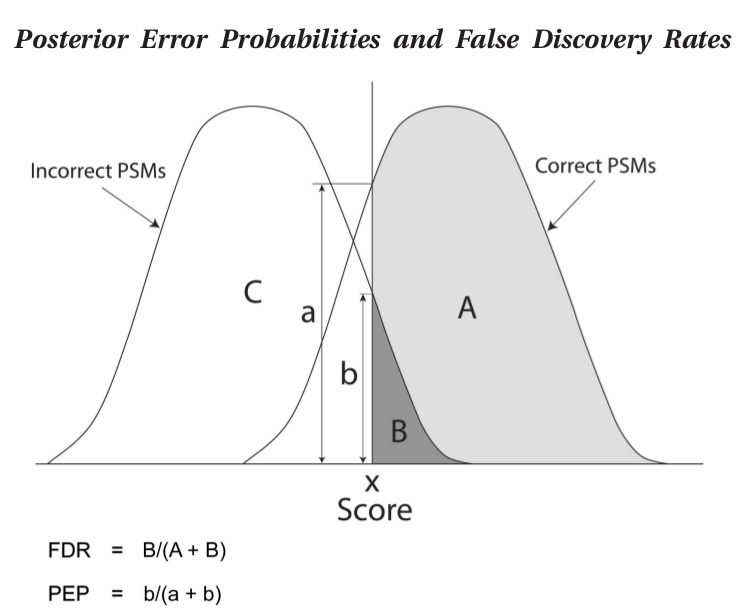
\includegraphics[width=0.9\linewidth]{pep}
\caption[FDR and PEP]{Visualizing FDR and PEP. The FDR at a given score \textit{s} is defined as the ratio between False Positives and the sum of True and False Positives found in the list of PSMs of score greater than \textit{s}. The PEP corresponds to the same ratio, but only at a specific score, hence its alternative name of local-FDR. Figure from \cite{Kall2008}.}
\label{fig:pep}
\end{figure}


The minimal FDR at which a given PSM is considered a valid match constitutes the PSM\textquotesingle s q-value, i.e it is the smallest FDR we can allow while still keeping the PSM \cite{Nesvizhskii2010}. Related to the q-value, the Posterior Error Probability (PEP) is an estimate of the probability of a given PSM of being an incorrect assignment (see figure \ref{fig:pep}). The PSM\textquotesingle s confidence is just defined as $1-PEP$ \cite{Nesvizhskii2010}. PEP can be computed from the decoy search results and provides another useful measurement of the uncertainty in the target results.




\section{Peptide and protein inference}
\label{sec:inference}

Two steps in protein identification can be distinguished:

\begin{enumerate}

\item \textbf{Peptide inference}: infer the peptides present in the sample.
\item \textbf{Protein inferece \textit{proper}}: based on the inferred peptides, infer what proteins generated them. This is not trivial as peptides are degenerate and frequently map to more than one protein.
\end{enumerate}

The result of the PSM step returns the inferred list of peptides. The ensemble of proteins most likely to have generated the list of peptides stemming from the filtered PSMs can be inferred using different algorithms. The degenerate nature of peptides is dealt with the Occam\textquotesingle s razor principle, which states that the most likely solution is the simplest one. Thus, protein inference algorithms aim at explaining the maximum amount of peptides using the least amount of proteins.

\section{Protein quantification}
\label{sec:quantification}

The combination of all the aforementioned computational analyses yields a list of protein identities that reports the protein composition i.e qualitative information of the original sample. However, in most proteomics applications, quantitative data can be of great interest, as many biological phenomena are manifested mainly through changes in the protein abundances, cell compartments, rather than the simple dichotomy of the protein\textquotesingle s existence \cite{Barsnes2008}. For instance, cancer cells in response to a drug could modulate the abundance of several proteins without removing them from the cytosol or introducing new ones.

Protein quantification pipelines can be classified based on whether isobaric labelling was used (label-based) or not (label-free). These are explained in subsection \ref{subsec:labelling}. If the label-free approach is employed, more distinctions can be made based on:

\begin{itemize}
\item The proxy used for quantification: spectral counting (\ac{SC}) or extracted ion currents (\ac{XIC}). These are explained in \ref{subsec:scvsxic}


\item The way the data are brought to the protein level from the peptide level: summarization-based vs. peptide-based, explained in \ref{subsec:peptide_model}.
\end{itemize}

\subsection{Label-based and label-free approaches}
\label{subsec:labelling}

%CITE PAGE 237 COMPUTATIONAL METHODS 

Two paradigms exist in protein quantification: label-based and label-free. In label-based quantification, originally identical peptides from a number of different samples are made distinguishable by their masses via the incorporation of a label. All label-based methods simultaneously analyze several samples in each experiment, removing the difficulties associated with between-run variability \cite{Barsnes2008}. The finite number of "plexes" available for a given label sets the limit to how many samples can be differentially quantified \cite{Cox2014}. Different techniques, like Stable Isotope Labeling by Amino acids in Cell culture (SILAC) or Isotope-Coded Affinity Tags (ICAT), differ in the nature of the label and the way it is introduced. Most of them have potential limitations \cite{Patel2009}. This, together with the limited amount of samples that can be compared makes a case for label-free quantification.

In the label-free quantification approach, peptides from different samples are not labelled differently and are thus distinguished by their presence in different, independent \ac{MS} runs. In order to account for the introduced inter-run variability in peptide identifications and \ac{RT}, a match-between-runs (MBR) processing step can be carried out (see figure \ref{figure:moff_mbr}). 


\begin{figure}[!h]
\centering
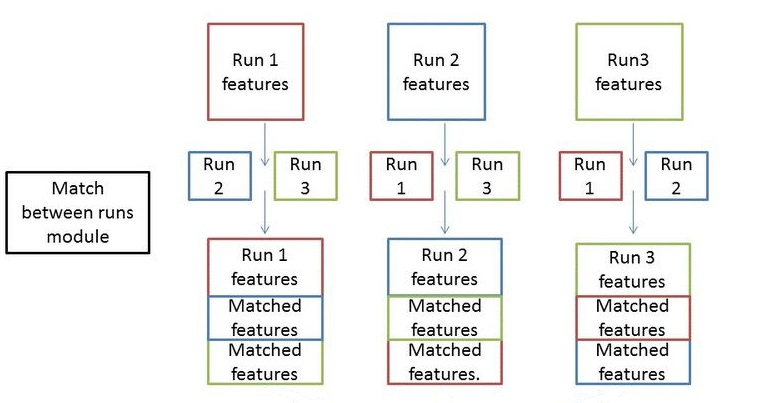
\includegraphics[width=0.9\linewidth]{mbr_workflow}
\caption[Match Between Runs module]{Illustration of the \ac{MBR} step. \textbf{A} the information gathered from matches in replicate runs is put to use during a reanalysis of the spectra. Modified from supplementary information in \cite{Argentini2016}.}
\label{figure:moff_mbr}
\end{figure}

This way, extra identifications are attained through a reanalysis of the spectra, factoring in the information collected in replicate runs. The RT and precursor mass of unidentified spectra in one replicate is matched to that of identified spectra in the remaining replicates. As a consequence, more identifications with a lesser fraction of missing datapoints are achieved.


\subsection{SC and XIC based quantification}
\label{subsec:scvsxic}


Quantification can be \ac{SC} or \ac{XIC} based.

On the one hand, spectrum counting based quantification is the simplest method in proteomics. The number of peptides a peptide is detected in the spectrometer is detected as proxy for its abundance. It relies on the rationale that highly abundant peptides will have a higher intensity and are thus more likely to trigger the acquisition of MS/MS spectra. These methods have the advantage that they are very simple to implement and don't require any further data processing \cite{Barsnes2008}.

On the other hand, \ac{XIC} based methods rely on intensity measurements at any level of the \ac{MS} workflow as proxies for protein abundance. A wide range of algorithms are available to process these data and output estimates of protein abundance. All of them require an intensive preprocessing step, usually including (I) taking the $log_2$ intensity to make the distributions symmetrical and thus fit for diverse parametric tests, and (II) quantile normalization to address between-runs variability in the intensity measurements. They can be classified in the bases of which MS level is used as proxy for the protein abundances and on whether or not a summarization step is performed to aggregate peptide-level data into protein-level data, or not. 


As stated in \cite{Cox2014}, \textit{although the abundance of proteins and the probability of their peptides being selected for \ac{MS/MS} sequencing are correlated to some extent, \ac{XIC}-based methods should clearly be superior to \ac{SC} given sufficient resolution and optimal algorithms. These advantages are most prominent for low-intensity protein/peptide species, for which a continuous intensity readout is more information-rich than discrete counts of spectra}. For this reason, only the \ac{XIC} approach will be regarded in the rest of the manuscript.  

For a more robust XIC based quantification, a feature extraction step is usually executed to extract consistent descriptors of identified peak clusters in the RT-m/z plance, as shown in figure \ref{figure:moff_apex}.

\begin{figure}[!h]
\centering
\begin{subfigure}{1\textwidth}
\centering
\caption*{A}
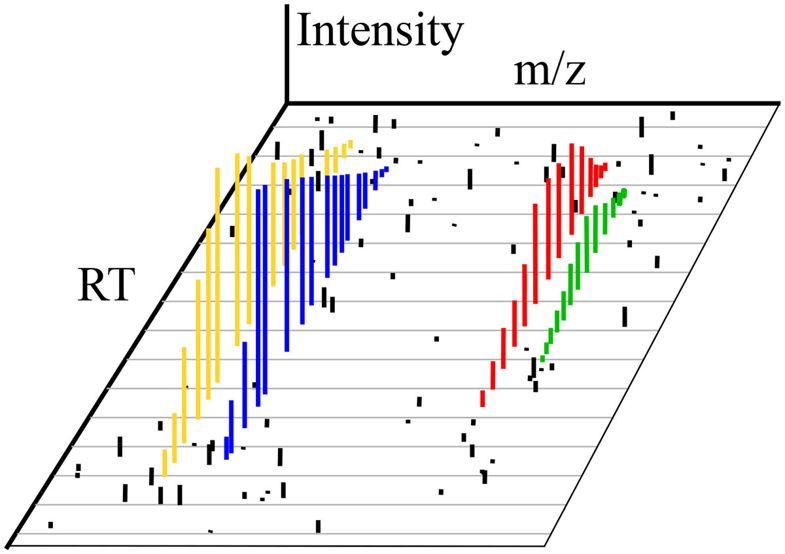
\includegraphics[width=0.7\linewidth]{apex_3d}
\end{subfigure}
\bigskip
\begin{subfigure}{1\textwidth}
\centering
\caption*{B}
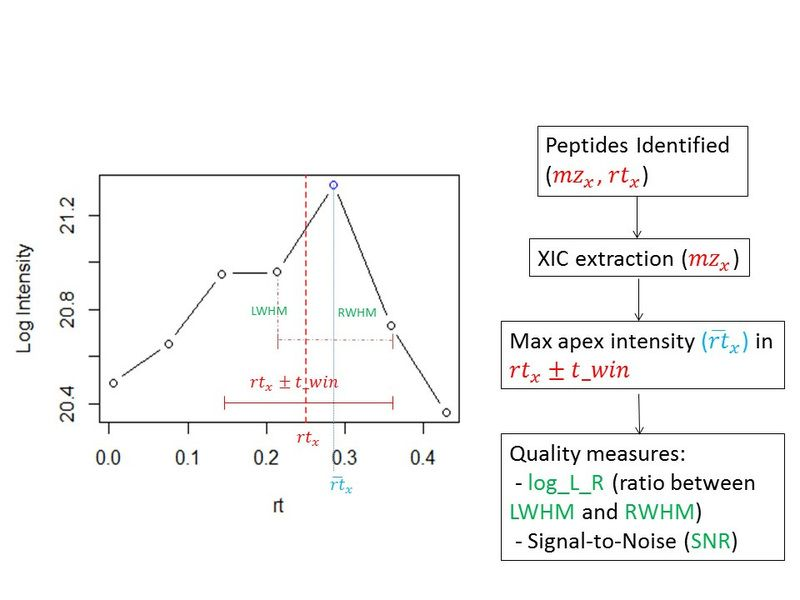
\includegraphics[width=0.7\linewidth]{apex_intensity}
\end{subfigure}
\caption[Apex MS1 intensity module]{Illustration of the apex intensity extraction step.\textbf{A} Visualization of a 3D peak cluster on the RT / m/z plane. An ion current at the same m/z ratio, thus corresponding to the same precursor ion, is detected with varying degrees of intensity over a more or less narrow time window, spreading the signal over time. Taken from \cite{Smith2014}. \textbf{B} A refinement analysis of these data attempts to fit a mathematical model of the signal over time and extract a representative measurement, such as the highest (apex) \ac{MS1} intensity. Modified from supplementary information in \cite{Argentini2016}.}
\label{figure:moff_apex}
\end{figure}


\subsection{\ac{XIC}-peptide-based models for label-free quantification}
\label{subsec:peptide_model}

The data collected in the mass spectrometer refers to peptides originating from a latent protein composition, given by the original sample. However, the data interpretation requires the transfer of these peptide-level data into the protein level. This can be done by either (I) performing an aggregation of the peptide-level data, where a summary value of the peptide-level data is taken as representative for the protein-level data, or (II) performing the protein quantification directly at the peptide-level by means of linear regression models.

As stated in \cite{Goeminne2015} \textit{peptides originating from the same protein can indeed be considered technical replicates and theoretically should lead to similar abundance estimates. However, the summarization of the peptide intensities into protein expression values is cumbersome, and most summarization-based methods do not correct for differences in peptide characteristics or for the between-sample differences in the number of peptides that are identified per protein. This might introduce bias and differences in uncertainty between the aggregated protein expression values, which are typically ignored in downstream data analysis steps}.

It is for this reason that peptide-based models offer the statistical framework required to learn as much from the data as possible. This translates into improved results when compared to the other aforementioned methods \cite{Goeminne2015}. %This hypothesis is the motivation for the method explained in chapter \ref{chap:model}.
\chapter{A label-free quantification proteomics pipeline}
\label{chap:pipeline}


\section*{Summary}

A pipeline making use of the tools SearchGUI \cite{Barsnes2018}, PeptideShaker \cite{Vaudel2015}, moFF \cite{Argentini2016} and MSqRob \cite{Goeminne2016}, was developed to support complete label-free protein quantification analyses using the most recent advances in the field with open-source software. The pipeline can be run on Linux computer clusters to perform (I) peptide to spectrum matching against a reference database, (II) quality control and filtering, (III) protein inference, (IV) \ac{MBR} and feature extraction, and (V) relative quantification. Its output can be passed to follow-up analyses in online databases or Bioconductor to get a biological interpretation of the results.  A benchmark of its performance was accomplished using the proteome benchmark dataset published in \cite{Cox2014}. The results were comparable to those achieved by the MaxQuant \cite{Cox2014} software, excepting a bias produced by the sample fractionation of this dataset.


\section{Introduction}

\subsection{Background}

Several proteomics pipelines are available under different licensing conditions. Many are released as closed-source commercial software, where information on how the program works is kept from the user. This is a serious drawback as it hinders the study of the implemented models and its customization. Open-source, free alternatives, like the Trans Proteomic Pipeline (\ac{TPP}) \cite{Deutsch2011} or openMS \cite{Sturm2008} are nevertheless available for the community, but they either lack good documentation, a broad user base or format exchangeability. MaxQuant, a freeware but closed-source, monolithic proteomics analysis suite \cite{Cox2008}, is developed for Windows and has only very recently been ported to Linux \cite{Sinitcyn2018}. Nevertheless it has been extremely successfully adopted by the scientific community due to its ease of use and comprehensive pipeline. The organization of a pipeline with comprehensive documentation, open-source nature, and easy implementation and customization was asserted to be lacking in the literature.

\subsection{Goals}

The development of a pipeline attempting to achieve the following goals will be described in this chapter.

\begin{enumerate}

\item Fully command line, documented and Linux-supported interface for easy automation and scalability.
\item Open-source for easy customization and extension.
\item Free-licensed and cost-free, so anybody with the knowledge can run it, democratizing the analyses.
\end{enumerate}

\section{Materials and Methods}

\subsection{Data generation and loading}

The proteome benchmark dataset \cite{Cox2014} was reanalyzed starting at the output RAW files available at the PRIDE repository \footnote{\href{https://www.ebi.ac.uk/pride/archive/projects/PXD000279}{Link to the PRIDE repository entry https://www.ebi.ac.uk/pride/archive/projects/PXD000279}}. Briefly, the \textit{Homo sapiens} and \textit{E. coli (strain K12)} proteomes were mixed in 1:1 (condition L) and 1:3 (condition H) proportions, with 3 replicates for each combination. Moreover, each of the 3 replicates of the 2 conditions was analyzed over 24 fractions. This experimental setting thus generated a total of $2 \times 3 \times 24=144$ RAW files. One file was missing in the repository. The ThermoRawFileParser \footnote{\href{https://github.com/compomics/ThermoRawFileParser}{ThermoRawFileParser repository https://github.com/compomics/ThermoRawFileParser}} program was used to convert RAW files to the MGF open format. These files were used as input for the Compomics+Rob pipeline.

The MQ+LFQ pipeline results were obtained starting at the supplemental table 1 from the MaxLFQ publication \footnote{\href{http://www.mcponline.org/content/13/9/2513/suppl/DC1}{Link to the data http://www.mcponline.org/content/13/9/2513/suppl/DC1}} \cite{Cox2014}, which are available as an excel file. The results of the MQ+Rob pipeline employed the Levenberg-Marquardt-minimised peptide intensities stored in the peptides.txt file contained in the spectraHeLaEColi.zip in the supplemental data.

%\href{http://www.mcponline.org/content/suppl/2014/06/17/M113.031591.DC1/mcp.M113.031591-1.xlsx}{http://www.mcponline.org/content/suppl/2014/06/17/M113.031591.DC1/mcp.M113.031591-1.xlsx}.

\subsection{Decoy database preparation and search}
\label{subsec:database_preparation}

The spectra saved in the MGF files obtained in the previous step were passed to the MS-GF+ search engine \cite{Kim2014} by means of the SearchGUI \texttt{SearchCLI} tool version 3.3.3 \cite{Barsnes2018} utility. The search parameters were set using the \texttt{IdentificationParametersCLI}. In order to account for potential post-translational modifications, the search was conducted allowing for the following variable modifications: oxidation of M and deamidation of N and Q. Moreover, C carbamidomethylation was set as fixed modification. The enzyme was set to semispecific Trypsin, allowing for a non-tryptic cleavage on any side of the peptide. Up to two missed cleavages were allowed. The precursor tolerance was 10 ppm and the fragment tolerance 0.5 Da. 


The target database was created by combining the Uniprot proteomes for \textit{E. coli (strain K12)} (UP000000625) and \textit{Homo sapiens} (UP000005640), downloaded in June 2018. A database accounting for common contaminants was also factored in. The decoy database was created using the \texttt{FastaCLI} utility in SearchGUI by reversing all sequences in the target.

\subsection{Quality control and validation}

The SearchGUI results were filtered using the default built-in checks available in the PeptideShaker version 1.16.22 utility \texttt{PeptideShakerCLI} \cite{Vaudel2015} \footnote{\href{A summary of the validation filters in PeptideShaker https://github.com/compomics/peptide-shaker/issues/300}{A summary of the default filters in PeptideShaker: https://github.com/compomics/peptide-shaker/issues/300}}. By default, the FDR was set to 1\%. PEP and confidence statistics were computed using the PeptideShaker built-in algorithms. Output was extracted via the Default PSM report txt file, available in the \texttt{ReportCLI} utility.


\subsection{\ac{MBR} and Apex MS1 intensity extraction}

The moFF command line utility \cite{Argentini2016} was applied to (I) perform match-between-runs and (II) extract MS1 apex intensity of each peak cluster. This required passing the original RAW files, together with the Default PSM report from PeptideShaker. Output was exported to a peptide summary file, containing  one row per peptide and for every peptide, the detected apex intensity for each sample in a column

\subsection{Quantification}

Relative quantification i.e. the computation of $\log_2$(ratios), or logarithm base 2 fold changes, $\log_2(FC)$ (\ac{log2FC}) was performed using the MSqRob package \cite{Goeminne2016} by passing the peptide summary file from moFF (Compomics+Rob) or the peptides.txt from MaxQuant (MQ+Rob). Prior to quantification, the data was preprocessed using the \texttt{preprocess\_MSnSet()} function. In a nutshell, (I) MS1 apex intensities were $log_2$ transformed, (II) quantile normalized, (III) peptides belonging to protein groups that contained one or more proteins that were also present in a smaller protein group were discarded \cite{Goeminne2016}, and (IV) protein groups with only 1 peptide were dropped.

Once preprocessing is done, a ridge regression model with Huber weights and empirical Bayes estimation of protein variance, implemented in the \texttt{fit.model()} function, was fit to every protein individually. The peptide and fraction effects were considered random, while the condition was treated as a fixed effect. The significance of the treatment effect differences was assessed through a Student\textquotesingle s T test, implemented in the \texttt{test.contrast()} function. Only protein groups that could be unambiguously mapped to one of the organisms were considered for the analysis.

Quantification in the MQ+LFQ pipeline was executed using the LFQ intensity columns stored in the data file. Intensities were $\log_2$ transformed and averaged. The difference between conditions H and L was taken as estimate of the log2FC. Significance was evaluated by means of the two-tailed Welch Two Sample t-test implemented in the \texttt{t.test()} function in R. P-values were corrected using the FDR method implemented in the \texttt{p.adjust()} function in R with the "fdr" method.


\section{Results}

\subsection{Running the Compomics+MSqRob pipeline}

The pipeline consists of a series of bash, Python and R scripts calling the tools published by the Compomics and StatOmics groups at the University of Ghent (see figure \ref{fig:pipeline}). A parameter file must be created before running the pipeline.

\begin{minted}[mathescape,
               linenos,
               numbersep=5pt,
               autogobble=true,
               frame=lines,
               framesep=2mm]{python}


create_decoy_database.sh
search_validate.sh
mbr_apex.sh
Rscript MSqRob.R

\end{minted}

The scripts are available at \href{https://github.com/antortjim/Thesis-Code}{https://github.com/antortjim/Thesis-Code}.

\begin{figure}[!h]
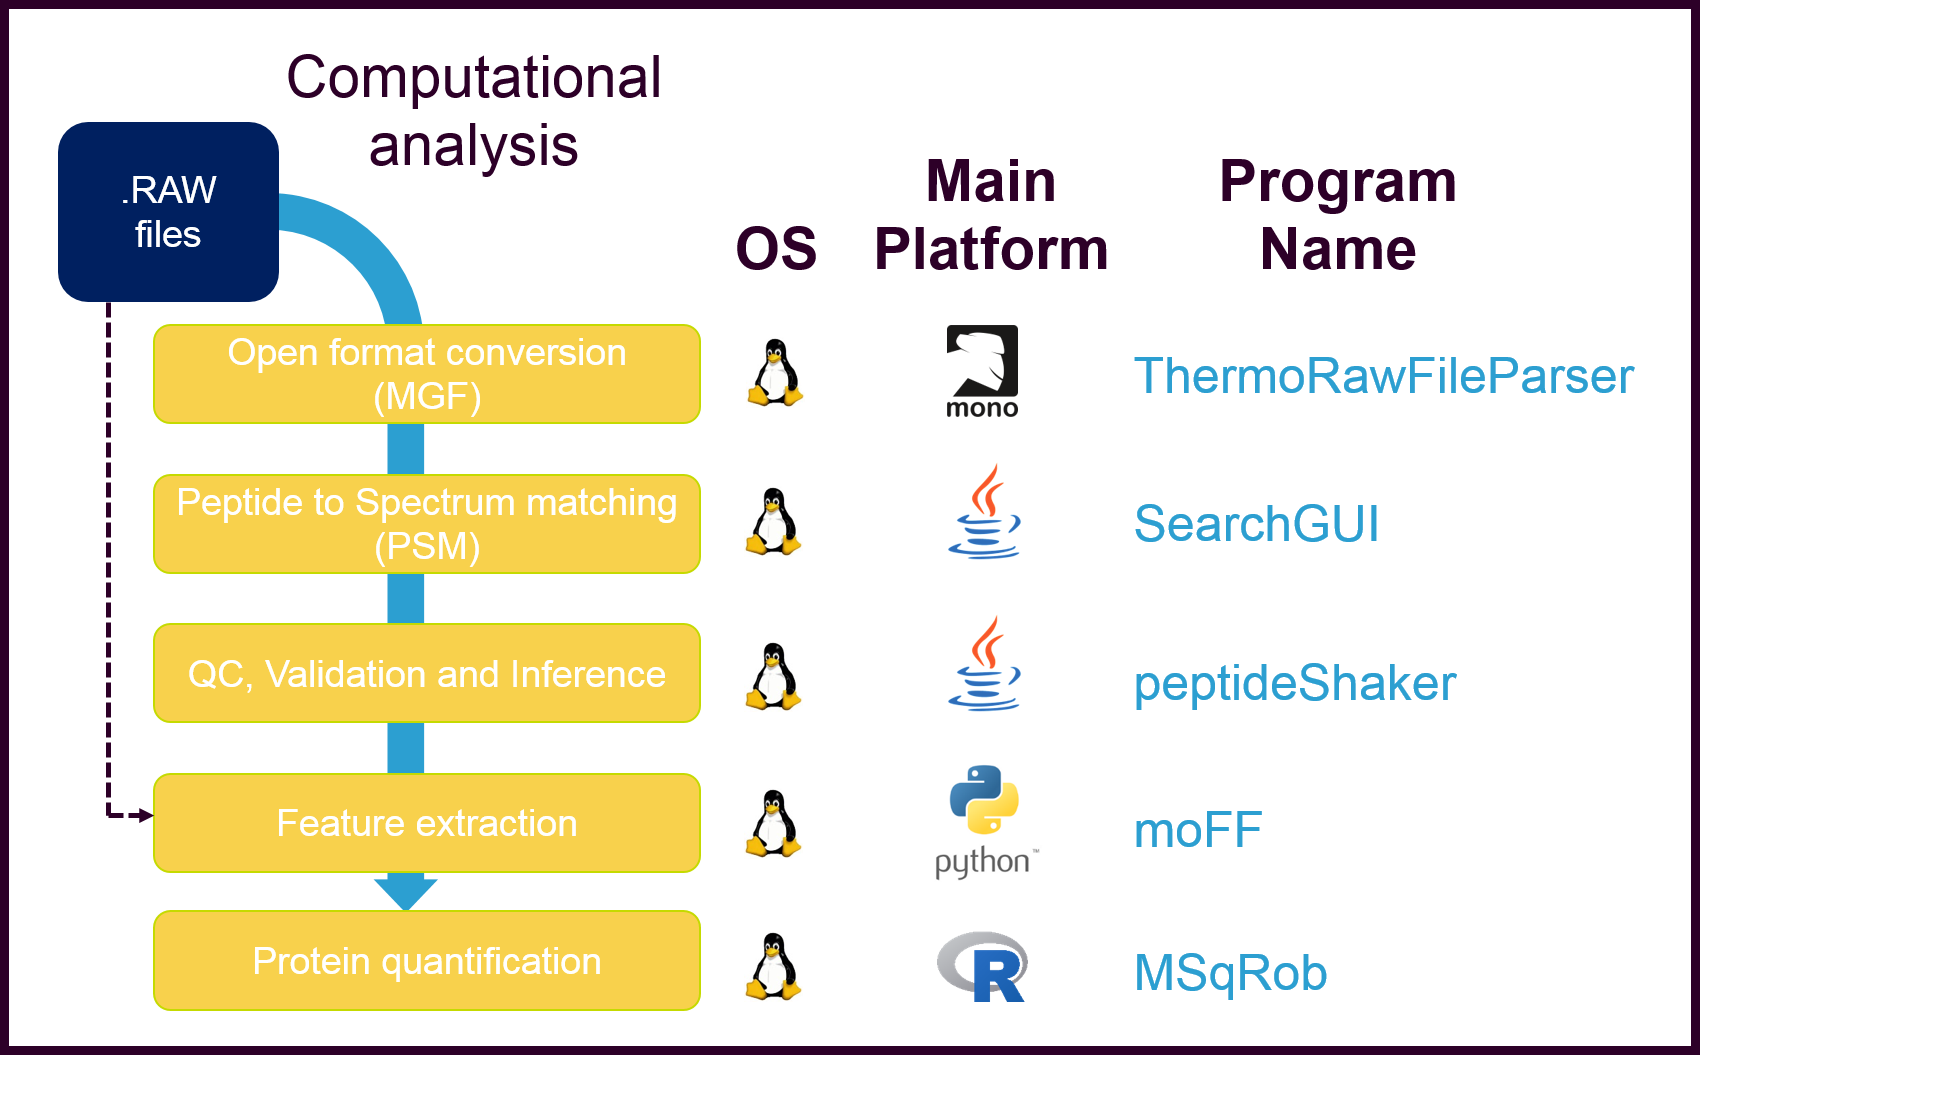
\includegraphics[width=\textwidth]{pipeline}
\caption[Schema of the presented pipeline]{\textbf{Schema of the presented pipeline}. .RAW files produced by the spectrometer are converted to an open format like the Mascot Generic Format (\ac{MGF}). After that, spectra are searched by means of a search engine to perform the PSM step. Thereafter, PSMs are validated and the most likely set proteins is inferred. If quantitative information is to be extracted, a quantification step attempting to estimate protein quantities is executed. The biological interpretation of the pipeline results can be achieved by interacting with public databases using R/Bioconductor or Python thanks to their open format.}
\label{fig:pipeline}
\end{figure}

\subsection{Evaluation of the PSM step}

The preprocessing of the RAW files produced by the mass spectrometer into the MGF open format enabled searchGUI to dispose of the registered spectra. PeptideShaker quality control and filtering capabilities carried out the required search results validation. As expected, matches to the target and decoy databases exhibited similar score distributions at low score values, while a divergence is observed at higher score values (see figure \ref{figure:qc_validation} A). Likewise, the m/z error was found to be closer to 0 on validated PSMs than on those which did not pass the 1\% FDR filter (see figure \ref{figure:qc_validation} C). The application of this filter implied that the FNR (false negative rate) was set to 5 \%, i.e 5 out of every 100 discarded matches were estimated to be true positives.



\begin{figure}[!h]
\centering
\begin{subfigure}{.45\textwidth}
  \centering
  \caption*{A}
  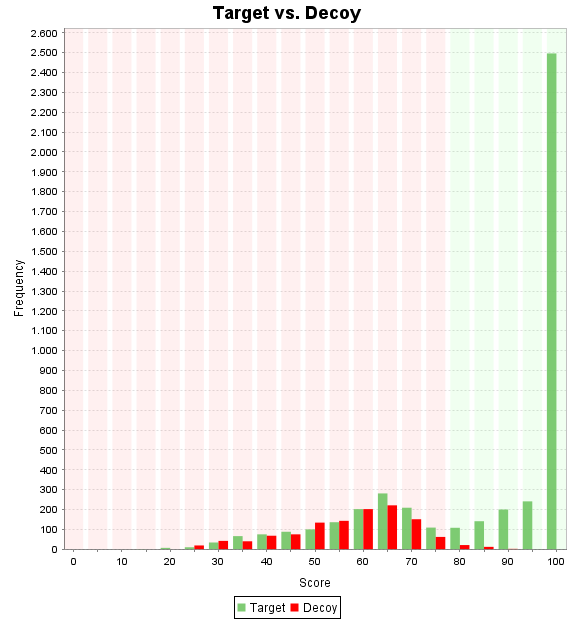
\includegraphics[width=.9\linewidth]{target_vs_decoy}
\end{subfigure}
\begin{subfigure}{.45\textwidth}
  \centering
    \caption*{B}
  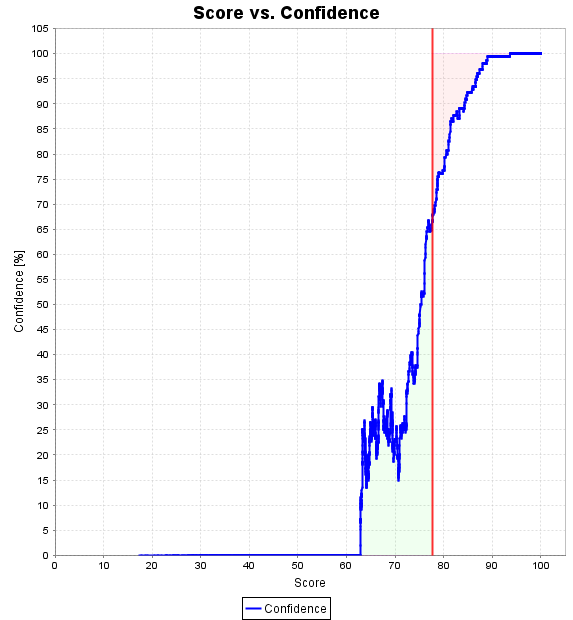
\includegraphics[width=.9\linewidth]{score_vs_confidence}
\end{subfigure}
\bigskip

\begin{subfigure}{.45\textwidth}
  \centering
    \caption*{C}
  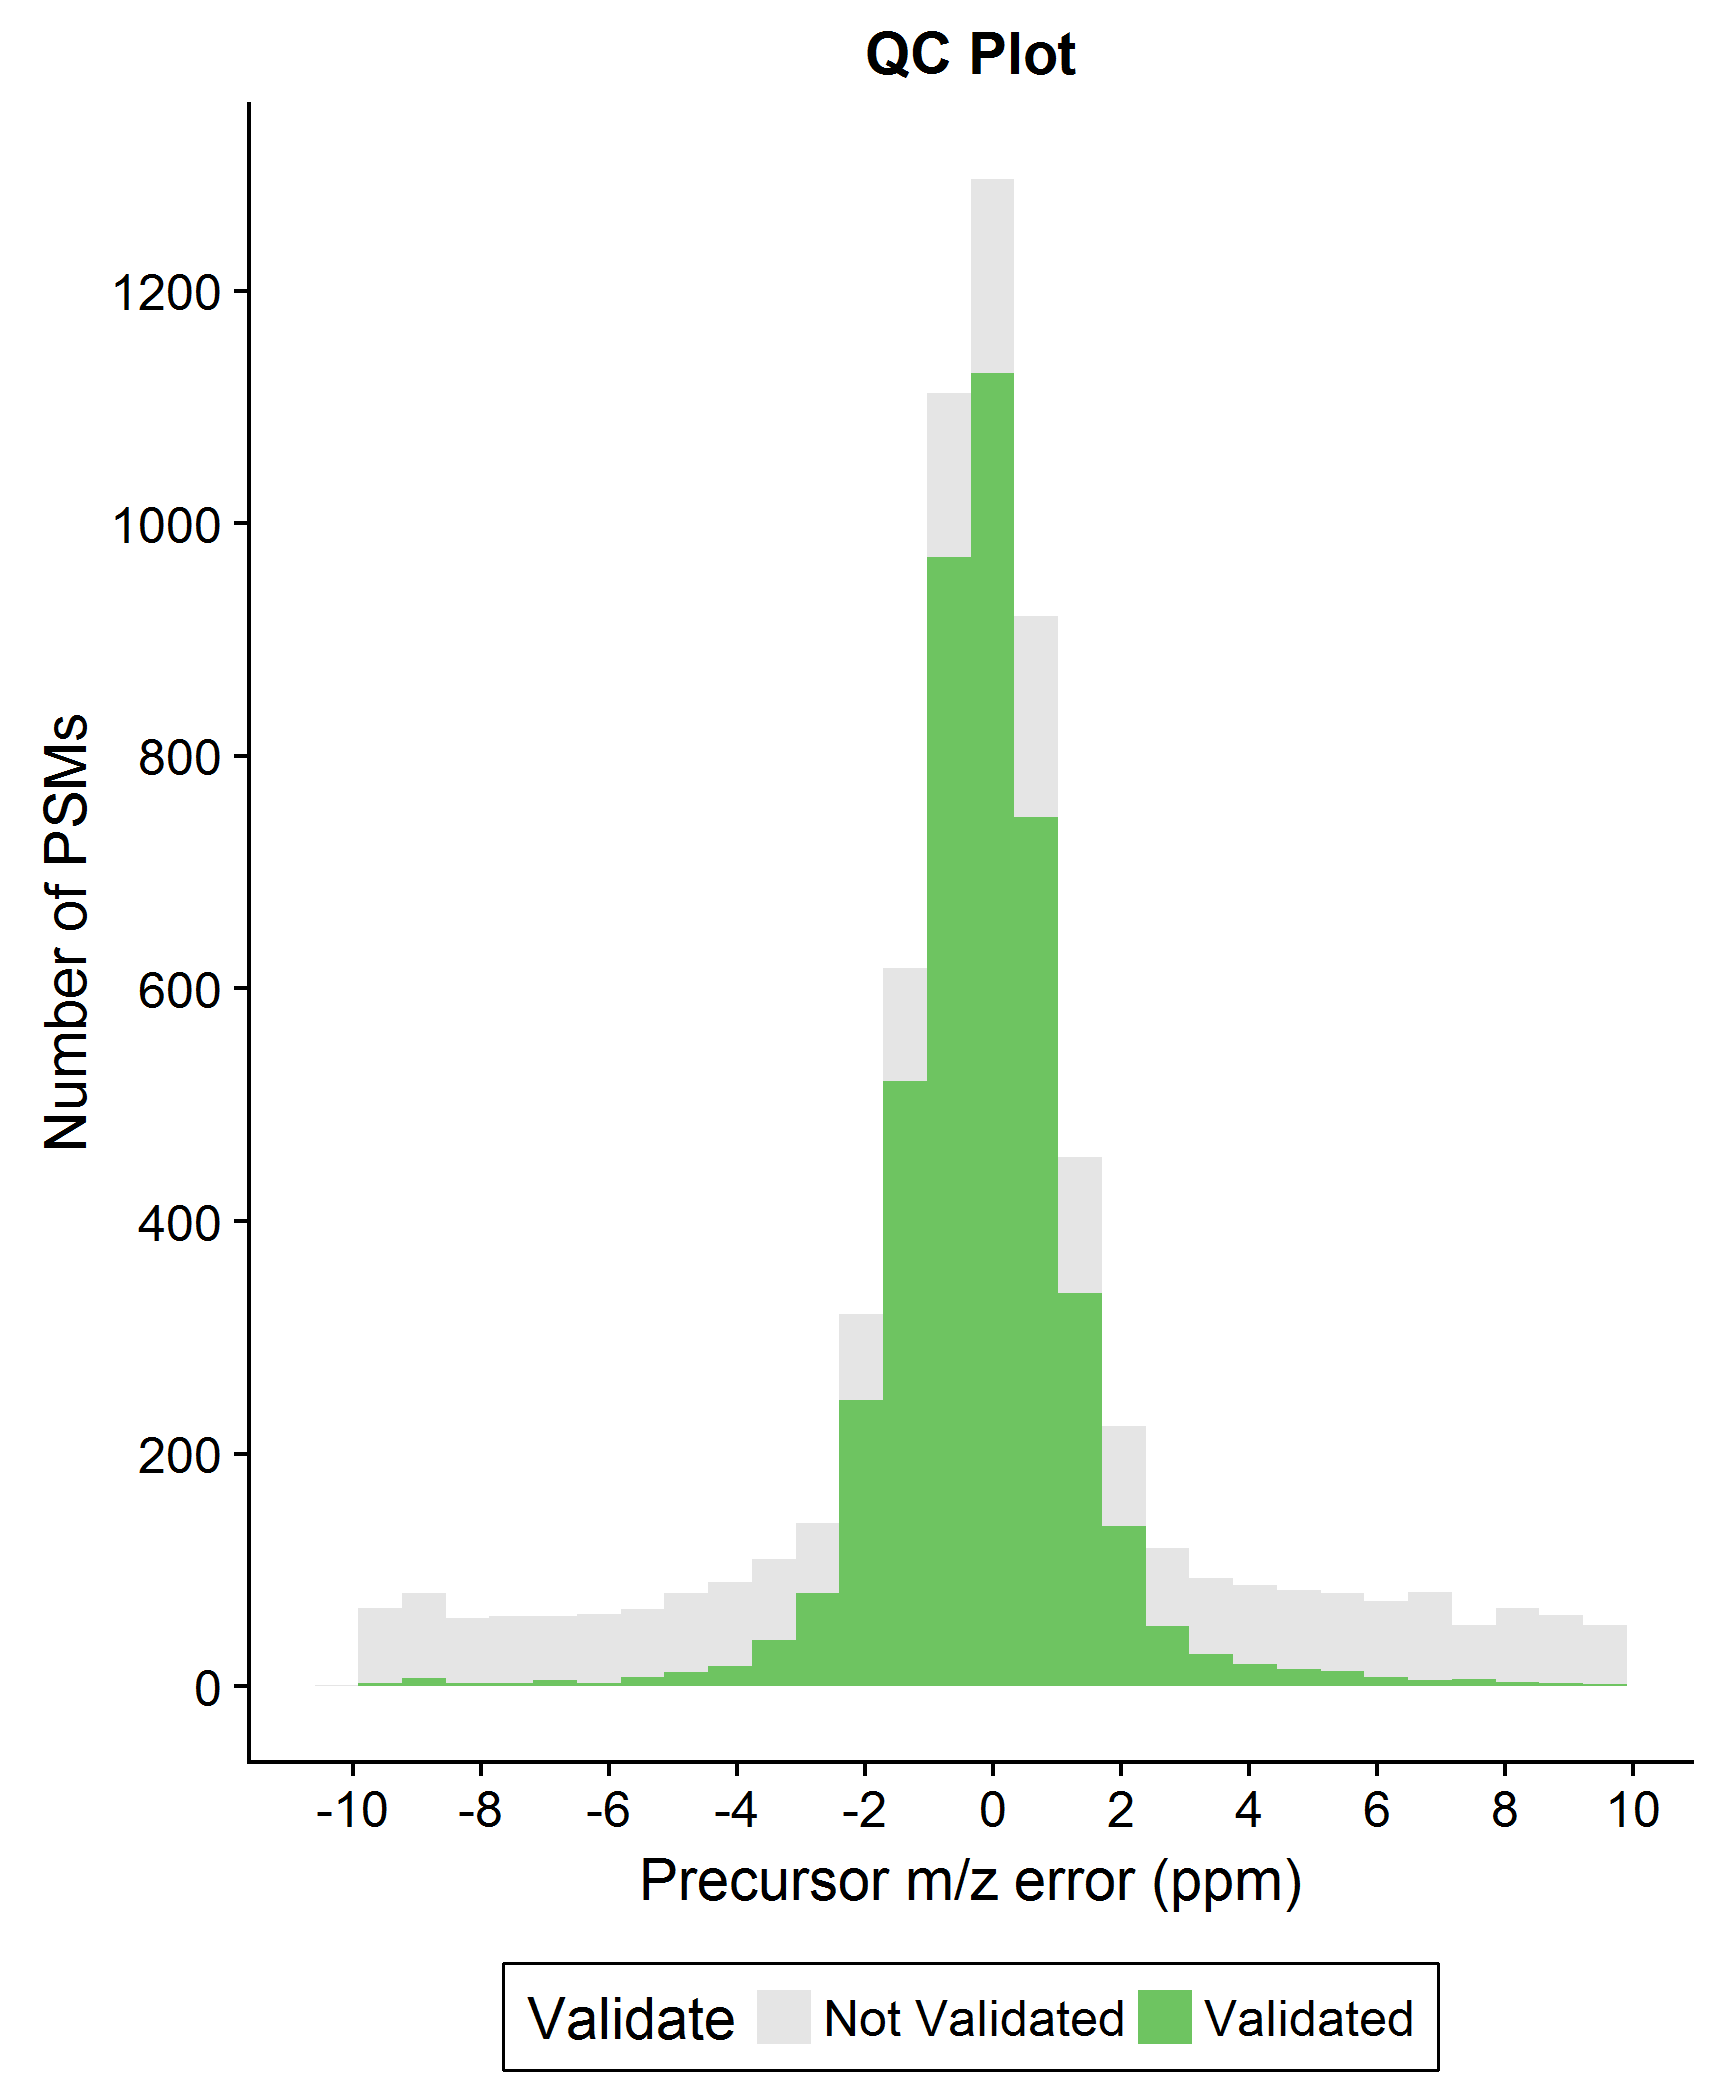
\includegraphics[width=.95\linewidth]{qc}
\end{subfigure}
\begin{subfigure}{.45\textwidth}
  \centering
    \caption*{D}
  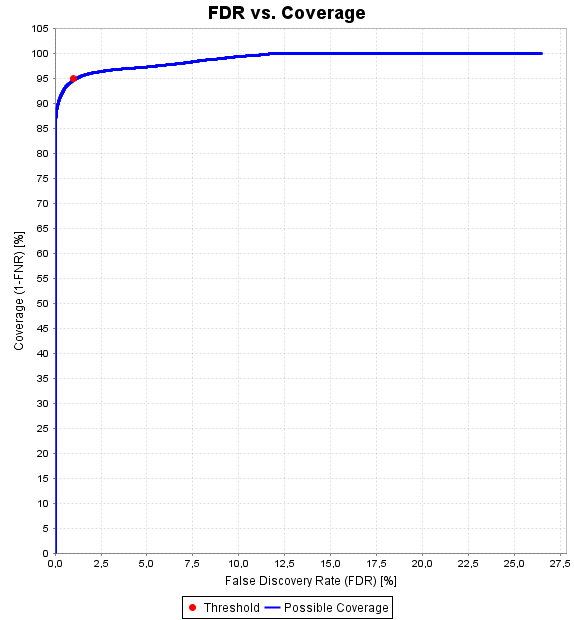
\includegraphics[width=.95\linewidth]{roc}
\end{subfigure}
\caption[Quality control and validation]{\textbf{QC and validation of the 13th fraction of the third replicate in condition L} \textbf{A} Score distribution for matches to the decoy and the target databases. \textbf{B} Evolution of the PSM score with confidence. The implemented cutoff at FDR of 1 \% is displayed with a red vertical line. \textbf{C} Distribution of the difference between the predicted and measured \ac{m/z} values, segregated by validation status. \textbf{D} ROC curve built upon the number of false positives and negatives estimated from the decoy search. The cutoff is displayed as a red dot.}
\label{figure:qc_validation}
\end{figure}

The 1\% FDR cutoff selected PSMs with a score higher than 78, which translated to a confidence (probability of the match being true) of at least 65\% (see figure \ref{figure:qc_validation} B).


The combination of both programs enabled the identification and validation (matching) of thousands of spectra with high confidence in all samples. However, when compared to the total amount of spectra available, the percentage of matched spectra was on average 37.4\%, with a marked decrease starting at fraction 14 (see figure \ref{fig:match_percent}).

\begin{figure}[!h]
\centering
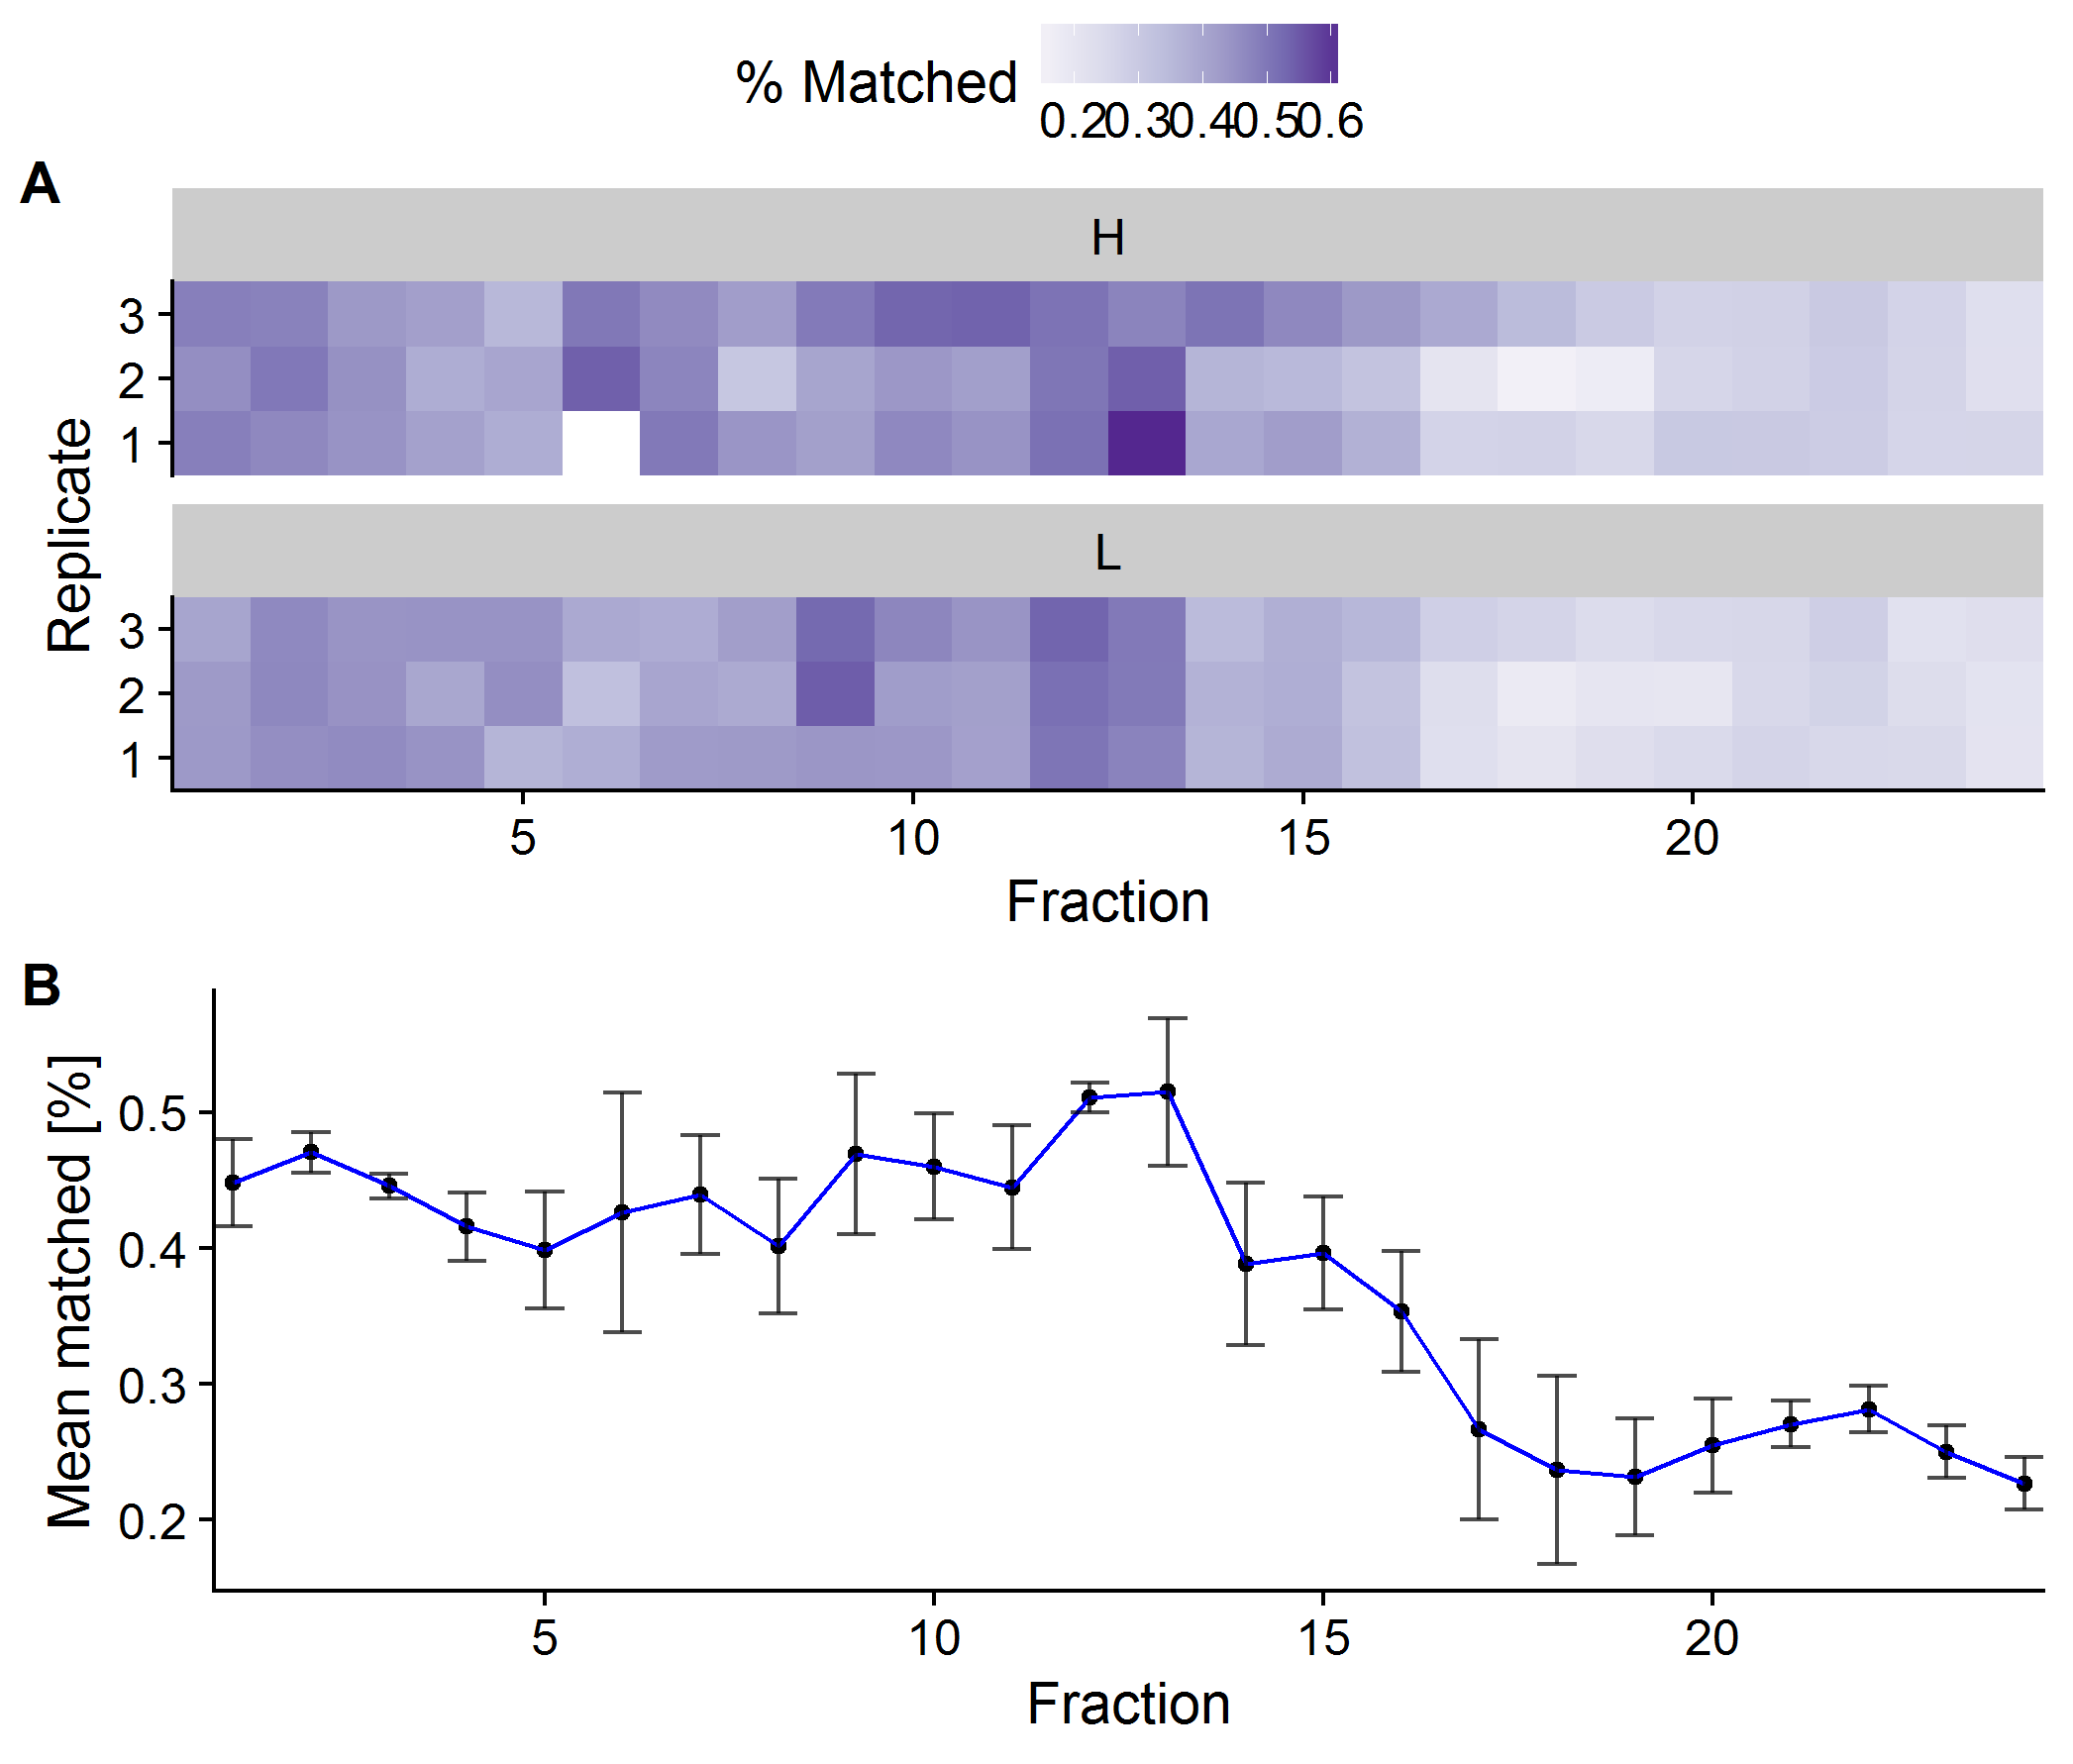
\includegraphics[width=0.8\textwidth]{match_percent}
\caption[Percentage of matched spectra in all samples]{\textbf{Percentage of matched spectra in all samples}. The total number of spectra per sample ranged between 5894 and 20249. \textbf{A} Percentages are encoded with a blue palette, the darker, the higher, and vice versa. The sixth fraction of the first replicate in condition H was missing in the PRIDE data repository. \textbf{B} The mean for each analysed fraction across conditions and replicates is displayed together with error bars to represent the standard deviation.}
\label{fig:match_percent}
\end{figure}

\subsection{Protein inference}

\begin{table}[H]
\begin{tabular}{ccccc}
  \toprule
 Total peptides & Unique peptides & Non-unique & Proteins & Protein groups \\ 
  \midrule
 46595 & 27384 & 19211 & 25056 & 10039 \\
 \bottomrule
\end{tabular}
\caption[Protein inference results]{Protein inference results. The counts of the different molecular entities detected by peptideShaker are displayed.}
\label{tab:protein_inference}
\end{table}

A total of 46595 peptides were identified in at least one of the fractions (see table \ref{tab:protein_inference}). Of them more than 27 thousand mapped to a unique protein (\textit{unique peptides}). However, a significant amount mapped to more than one protein (\textit{degenerate peptides}). Such peptides are called non-unique peptides. The 25056 detected proteins were grouped into 10039 protein groups. Protein groups are peptide generating entities for which enough data is available to confirm the presence of at least one of them, but not to precisely assess which of them.

Protein groups are very frequent due to several factors. For example, protein isoforms, consisting of protein sequences differing in potentially only one aminoacid, are very difficult to resolve. PeptideShaker executes a smart protein grouping by harnessing the annotation of proteins and classifying protein groups based on how well the annotation backs the protein group \cite{Vaudel2015}. However, in the present analysis the quality of the protein group was not taken into account, as explained in the Materials and Methods.


\subsection{MBR and apex intensity extraction evaluation}

The match-between-runs (\ac{MBR}) step allowed for increased identifications by transferring successful matches between replicate runs. The results of this process for the 13th fraction of the L condition is shown in figure \ref{fig:mbr}.

\begin{figure}[H]
\centering
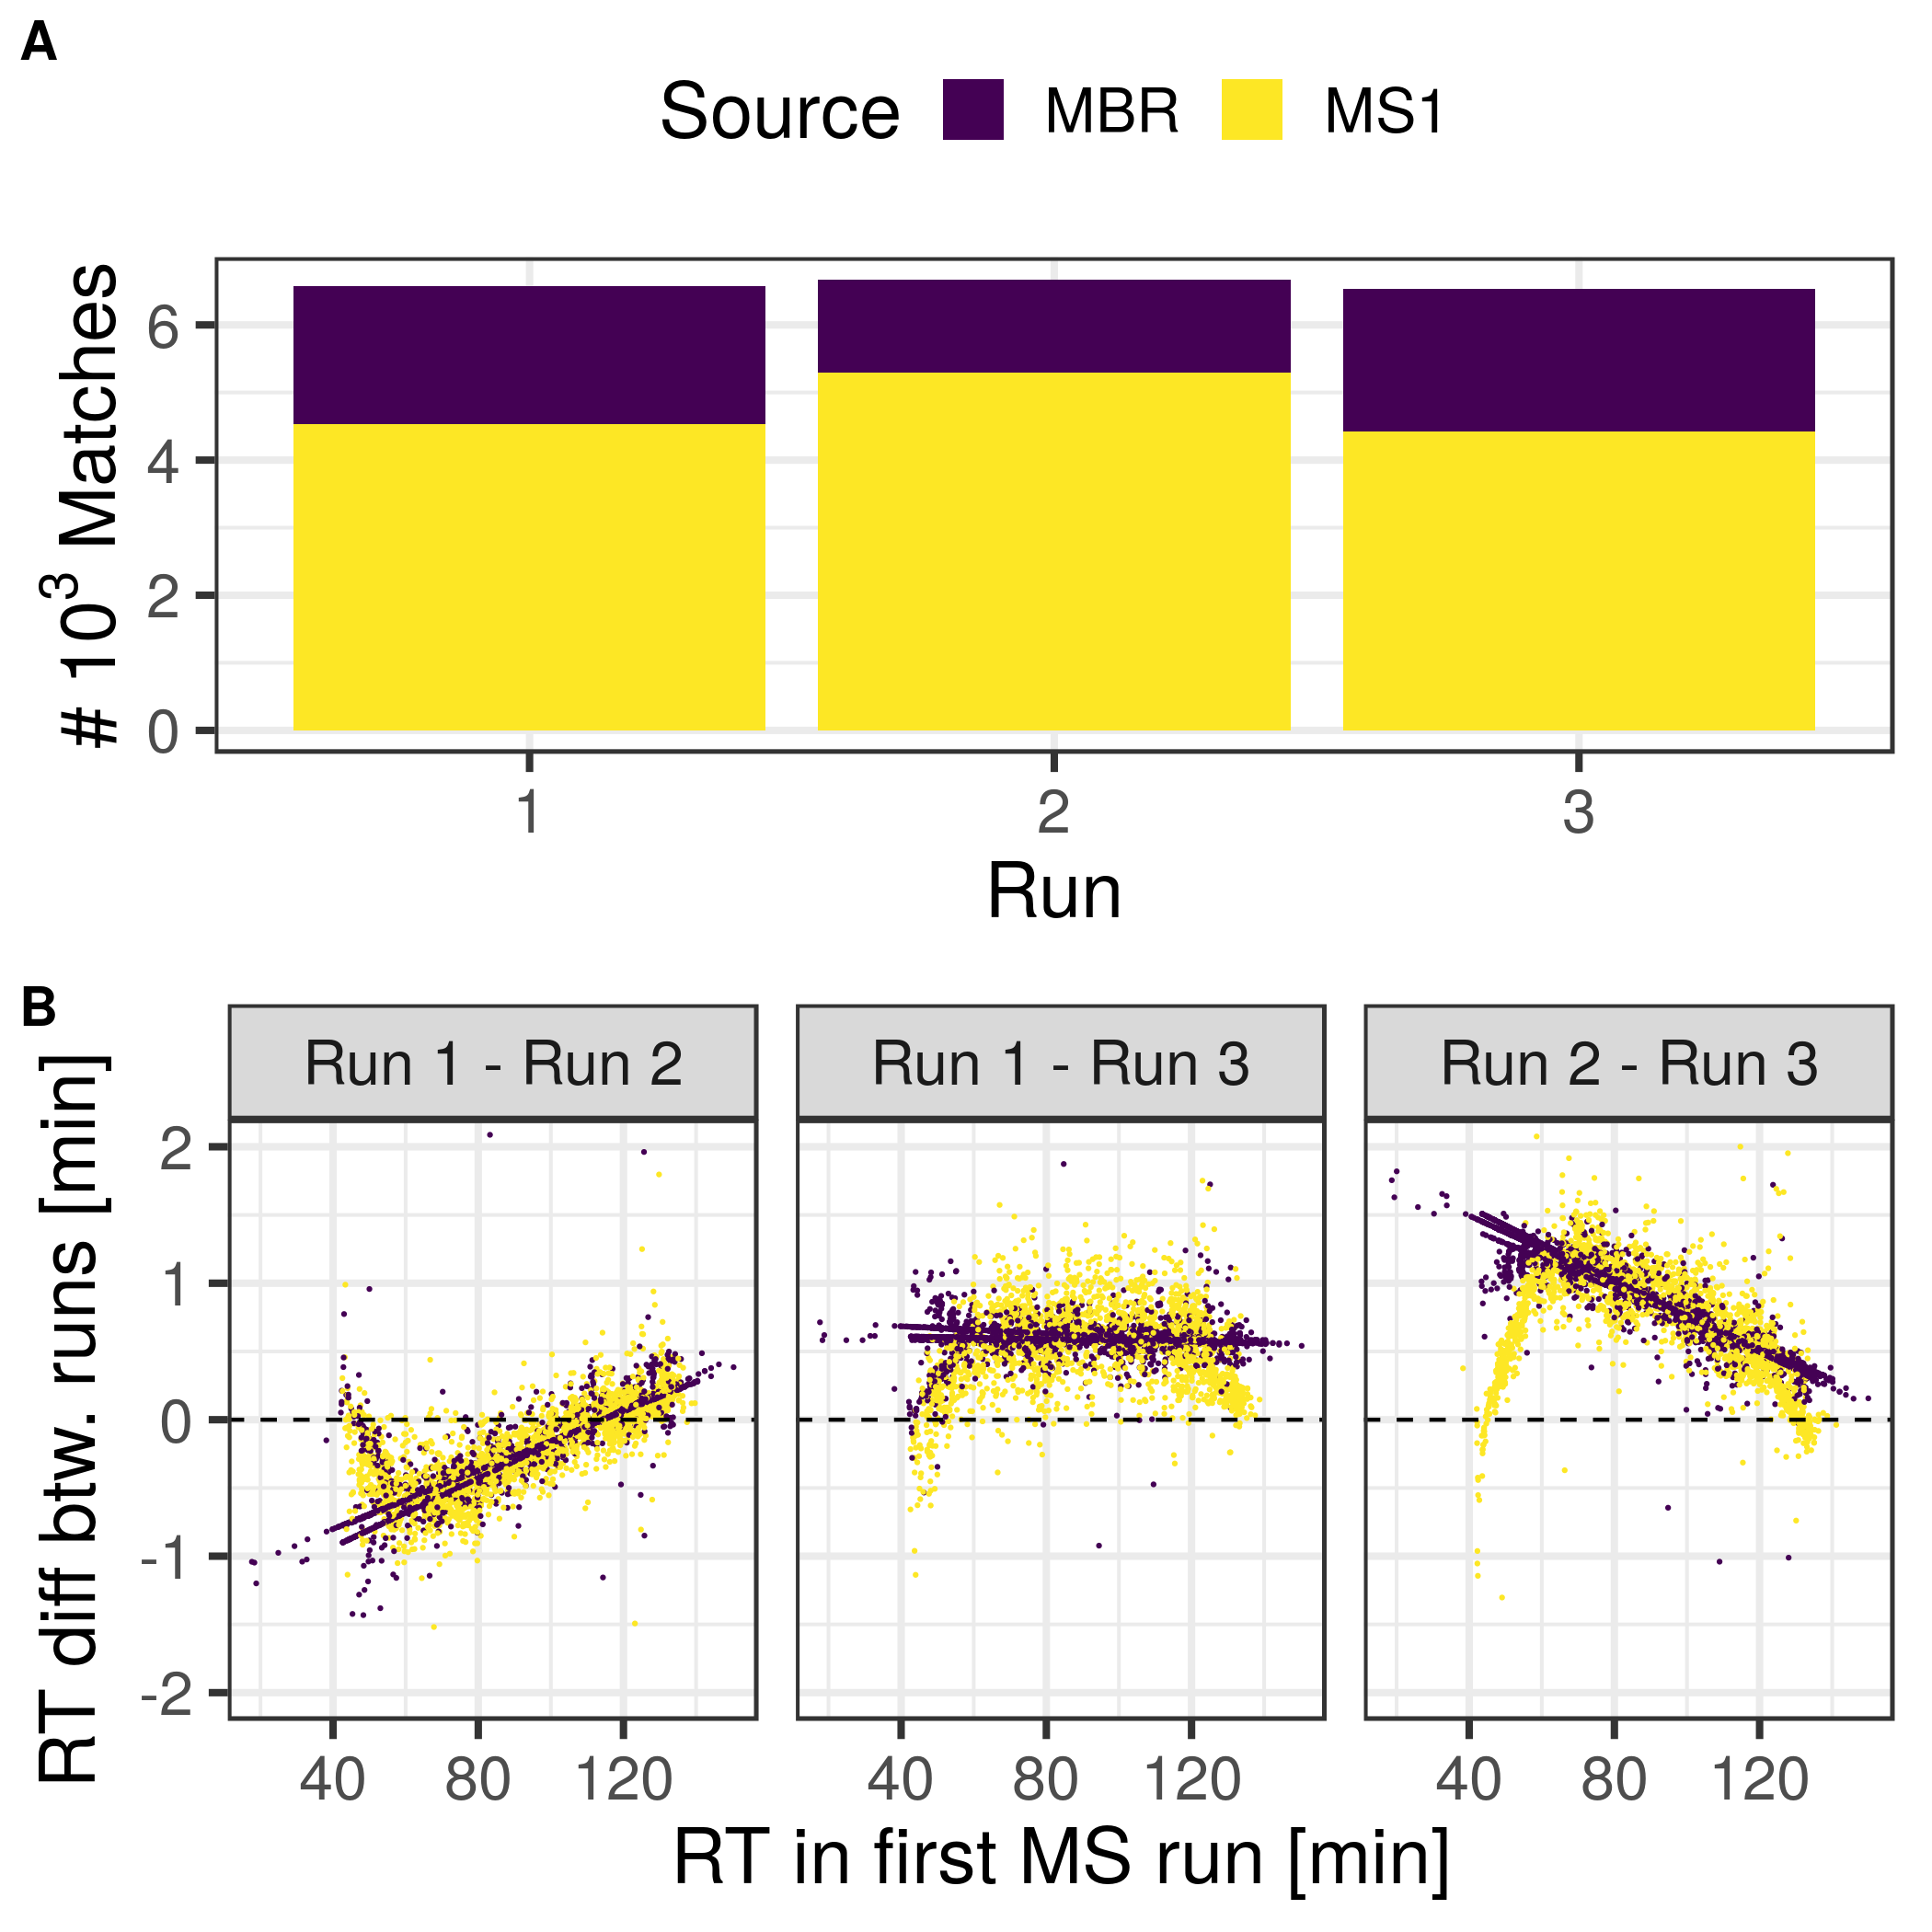
\includegraphics[width=\textwidth]{mbr_combined}
\caption[Proteome benchmark MBR results]{Match Between Runs with moFF. \textbf{A} Count of identifications on each run segregated by source. More than 4k spectra were identified and validated by SearchGUI+peptideShaker. In this particular case, hundreds of new identifications were accomplished via moFF. \textbf{B} Match visualization. Every dot represents a peptide shared across 2 runs. The coordinate system illustrates its retention time on the first run on the x axis and the difference with the second run on the y axis. The color depicts whether the identification was carried out during the PSM process (MS1), or thanks to a cross-identification achieved by the MBR module (MBR).}
\label{fig:mbr}
\end{figure}

Once as many identifications as possible were gathered, a refinement of the measured MS1 intensity can be implemented to select the apex of every peak cluster, which yields robust intensity measurements for each sample (see figure \ref{fig:apex_intensity}). 

\begin{figure}[H]
\begin{subfigure}{.9\textwidth}
  \centering
    \caption*{A}
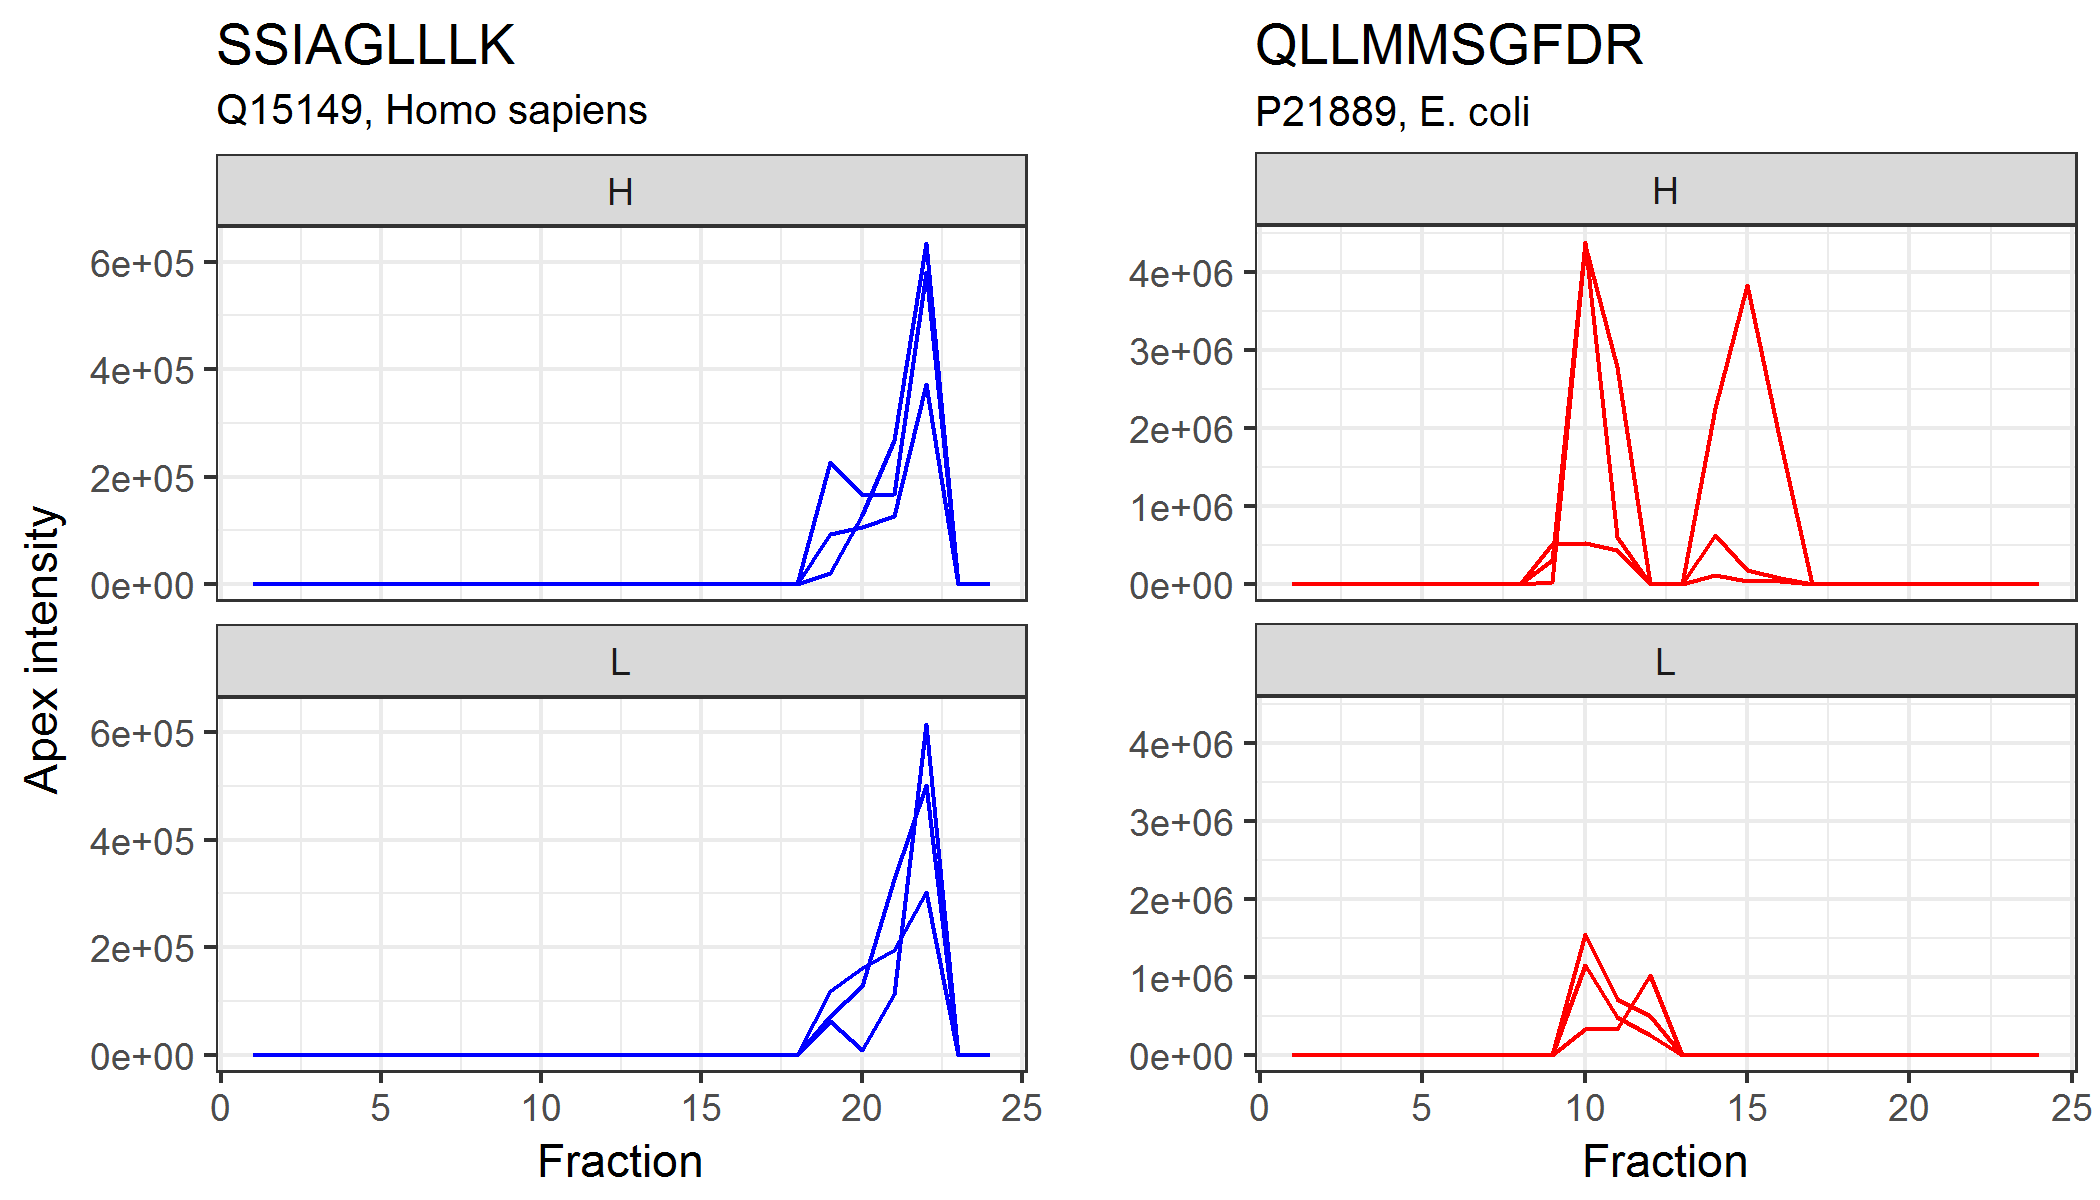
\includegraphics[width=.9\linewidth]{peptide_profile}
\end{subfigure}
\bigskip

\begin{subfigure}{.9\textwidth}
  \centering
    \caption*{B}
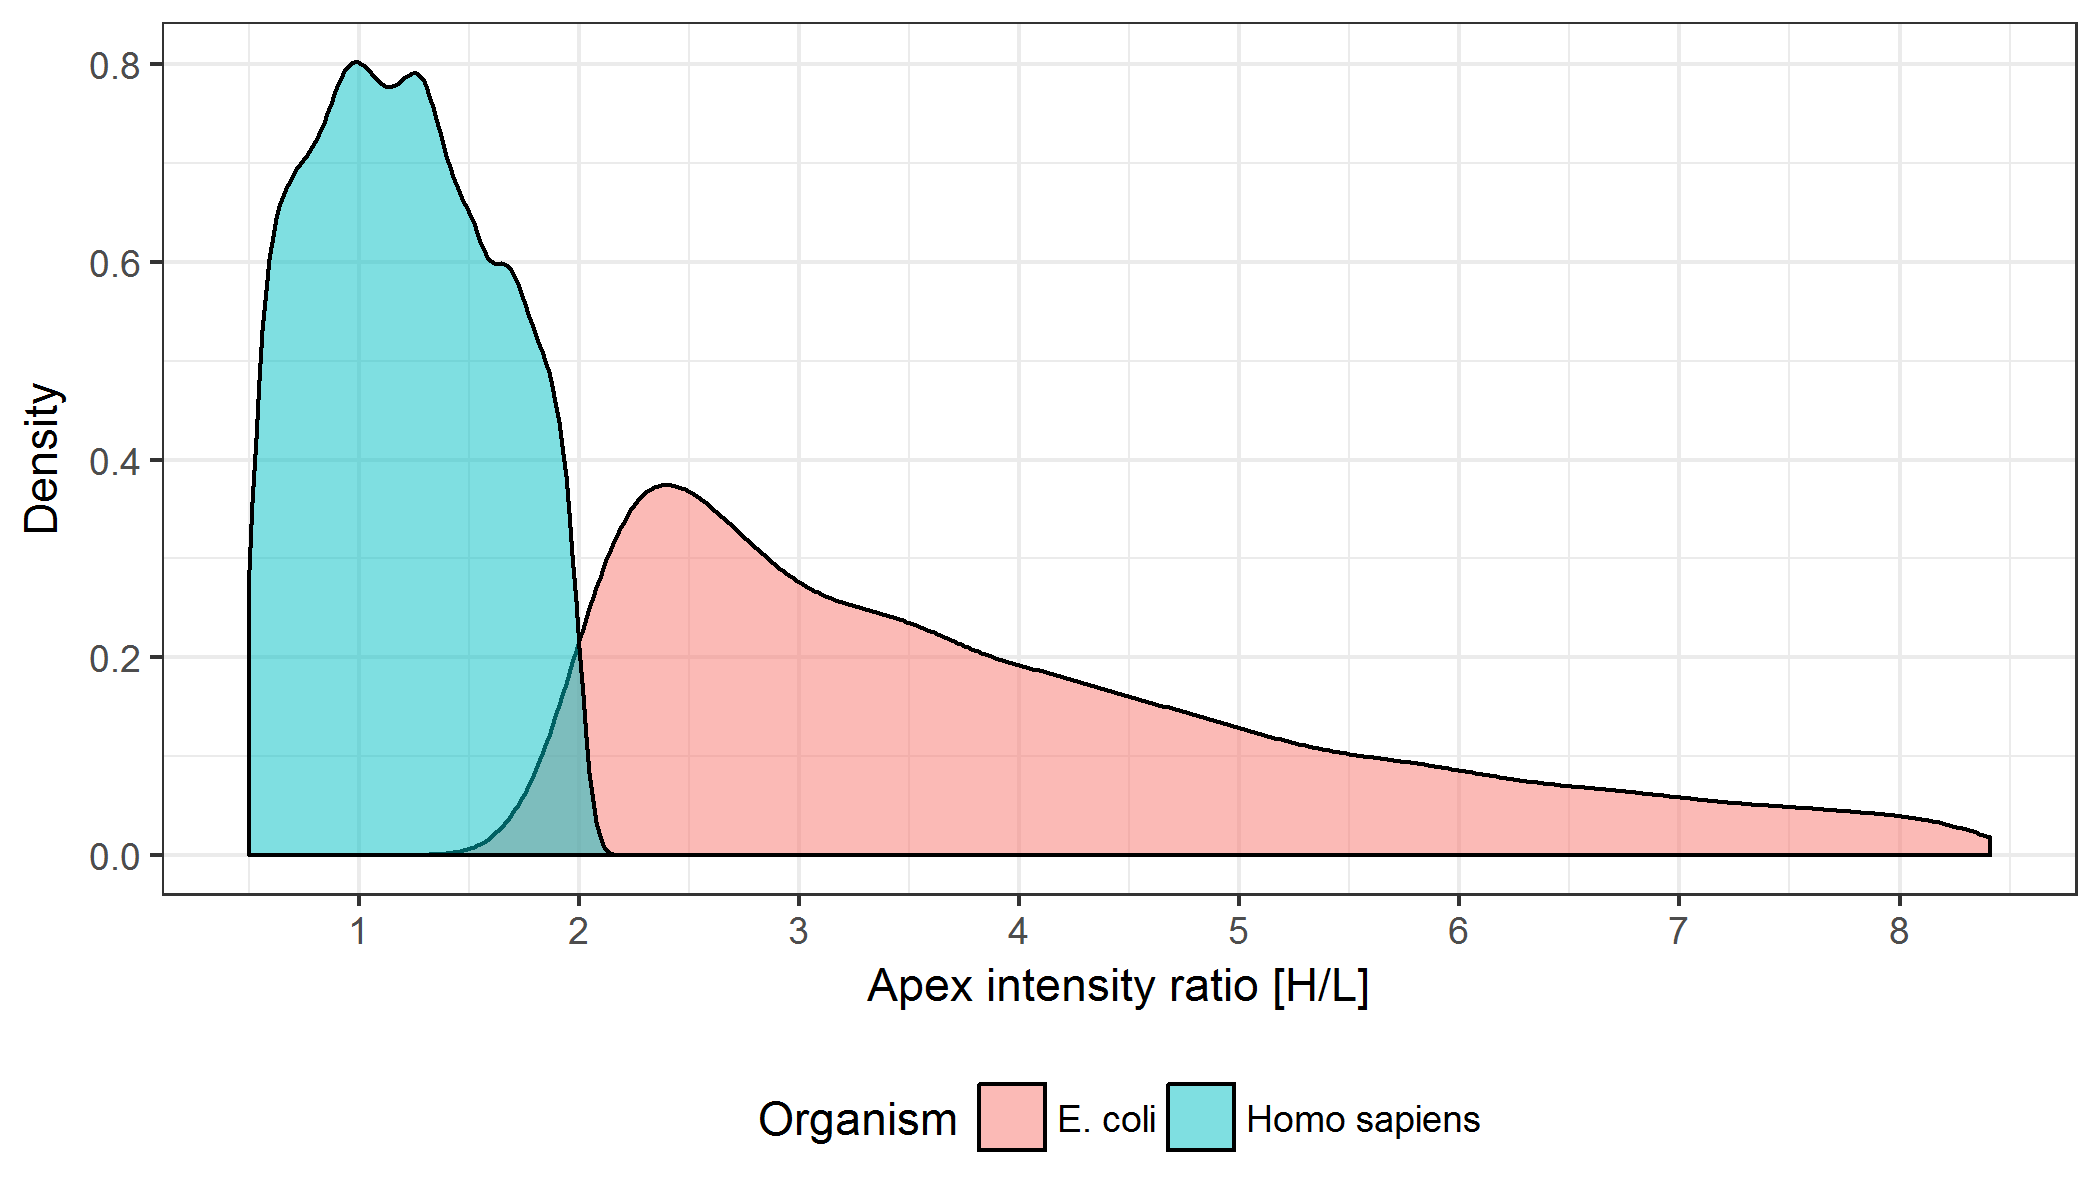
\includegraphics[width=.9\linewidth]{density_ratio}
\end{subfigure}
\caption[Proteome benchmark apex MS1 intensity results]{\textbf{A} The apex intensity profile across fractions for 2 different peptides, one from \textit{Homo sapiens}, and one from \textit{E. coli}. The figure illustrates the intrinsic intensity variability between technical replicates, particularly in the case of the \textit{E. coli} QLLMMSGFDR peptide, as it was almost non-existent in one of the runs. \textbf{B} The expected pattern of overall similar intensities for the \textit{Homo sapiens} data and 3-fold higher intensities for the \textit{E. coli} data in condition H was observed, confirming an acceptable performance of the protocol.}
\label{fig:apex_intensity}
\end{figure}


\subsection{Quantification benchmark}
\label{subsec:quantification}

Could the apex MS1 intensities extracted by moFF be used as proxy for peptide abundance and perform relative quantification? It is important to take into account as many of the effects influencing the recorded data as possible. In this case, besides the different H and L conditions, peptide, run and fraction effects could be distinguished. The MSqRob quantification engine treats effects differently depending on whether or not they are random or fixed. Fixed effects should have a consistent impact in the ion currents measured in the spectrometer, whereas random effects are truly random and thus unpredictable.

The result of the process was the successful quantification of 5307 protein groups out of 10039 (see table \ref{tab:quantification_table}).

% latex table generated in R 3.4.4 by xtable 1.8-2 package
% Sun Jul 15 18:17:23 2018
\begin{table}[ht]
\centering
\begin{tabular}{llll>{\itshape}l}
  \toprule
 & \ac{log2FC} & qval & Protein & Organism \\ 
  \midrule
1 & -4.76E-01 & 1.42E-24 & P78527 & Homo sapiens \\ 
   \rowcolor[gray]{0.95}2 & 6.80E-01 & 6.75E-24 & P0A8V2 & E. coli \\ 
  3 & 8.50E-01 & 4.39E-22 & P25516 & E. coli \\ 
   \rowcolor[gray]{0.95}4 & 7.07E-01 & 2.05E-18 & P63284 & E. coli \\ 
  5 & 1.04E+00 & 1.21E-17 & P37095 & E. coli \\ 
   \rowcolor[gray]{0.95}6 & 7.78E-01 & 1.51E-16 & P13029 & E. coli \\ 
  7 & 8.89E-01 & 5.62E-16 & P77804 & E. coli \\ 
   \rowcolor[gray]{0.95}8 & 8.53E-01 & 1.72E-15 & P23721 & E. coli \\ 
  9 & -6.97E-01 & 1.41E-14 & P09874 & Homo sapiens \\ 
   \rowcolor[gray]{0.95}10 & 1.37E+00 & 1.41E-14 & P37666 & E. coli \\ 
   \bottomrule
\end{tabular}
\caption[Proteome benchmark dataset quantification results]{Results of the quantification pipeline. The 10 protein groups with the lowest \textit{q-val}  as estimated by MSqRob are shown. Notably, eight correspond to proteins belonging to \textit{E.coli}. The two human proteins exhibited in both cases an absolute value of the \ac{log2FC} below 1.}
\label{tab:quantification_table}
\end{table}

The performance of the quantification can be evaluated thanks to the experimental design of the dataset. Since the \textit{E. coli} proteome was mixed on a 3:1 ratio in condition H, a \ac{log2FC} of $log_2(3)=1.58$ is expected for proteins coming from this organism. Likewise, human proteins should have a \ac{log2FC} of 0. As such, the evaluation can be reformulated as a classification task were the quantification algorithm tries to distinguish between one of the two organisms.


\begin{figure}[H]
\centering
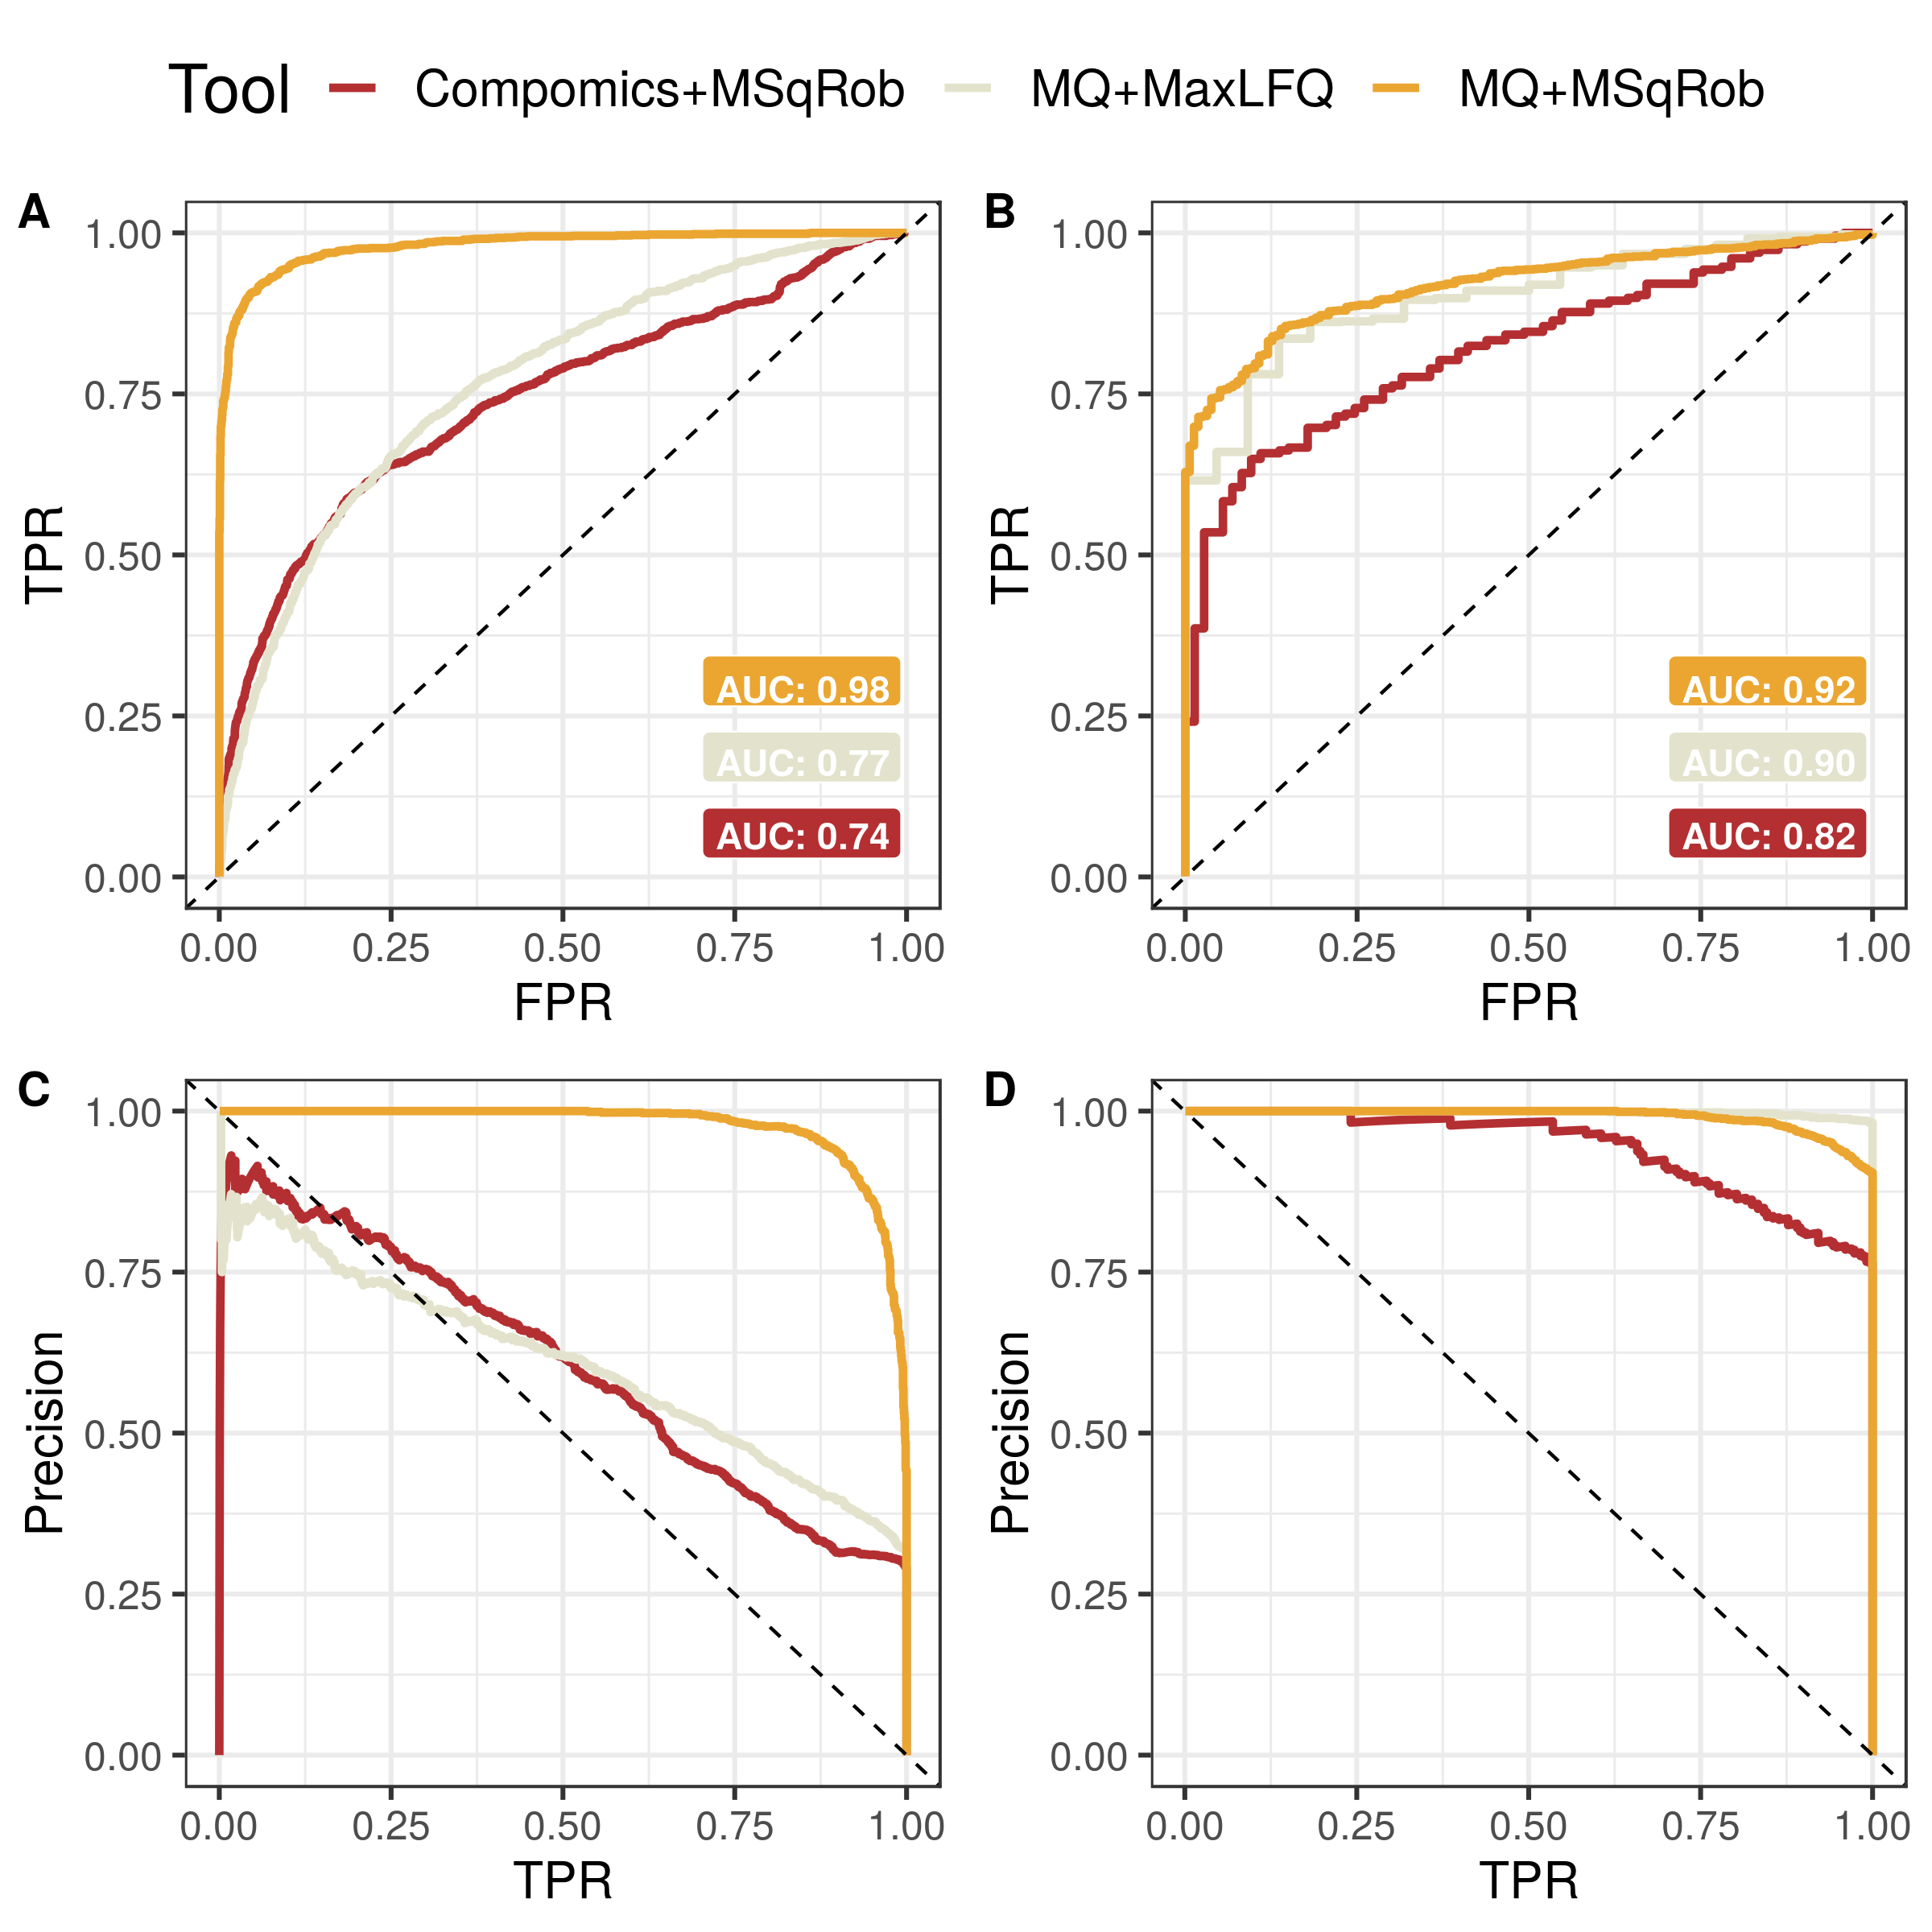
\includegraphics[width=\textwidth]{curves_plot}
\caption[Classifier evaluation: ROC and PR curves]{ROC and PR curves displaying the behaviour of 3 different label-free quantification pipelines publicly available. \textbf{Comp+Rob} is the pipeline presented in the previous sections. \textbf{MQ+LFQ} consists of a standard MaxQuant upstream analysis combined with its LFQ quantification engine. Finally, \textbf{MQ+Rob} blends MaxQuant upstream analysis with the MSqRob quantification engine. \textbf{A, B} ROC curve produced by the three algorithms with no \ac{log2FC} filter, and keeping proteins with \ac{log2FC} greater than 1, respectively. \textbf{C, D} PR curve produced by the three algorithms with no \ac{log2FC} filter, and keeping proteins with \ac{log2FC} greater than 1, respectively.}
\label{fig:roc_curves}
\end{figure}


Some of the most frequent evaluations of the performance of a binary classifier are the Receiver Operating Characteristic (ROC) and Precision-Recall (PR) curves \cite{Bradley1997}, which demonstrate the performance of the algorithm at different cutoff values of a predictor variable. Together, they show the False Positive Rate (FPR), the True Positive Rate (TPR) or recall, and the precision exhibited by the algorithm.




In the present problem, they can be used to show how well the \textit{q-value} separates the two classes (organisms). Thus, \textit{E. coli} proteins are treated as positives, and those from \textit{Homo sapiens} are treated as negatives. Moreover, a filter based on the \ac{log2FC} can be applied to enrich the data in positives and facilitate the classification task.

In order to compare the results of the here presented pipeline (Comp+Rob) with those achieved by other available tools, the analysis was repeated using the data processing implemented in MaxQuant \cite{Cox2008} at different steps. The pipeline combining MaxQuant and MaxLFQ (MQ+LFQ) was fully carried out using the MaxQuant suite, whereas the combination of MaxQuant and MSqRob (MQ+Rob) used MaxQuant without its quantification engine MaxLFQ.

The result of this analysis is shown in figure \ref{fig:roc_curves}. Remarkably, Comp+Rob achieved similar results to those resulting from MQ+LFQ. Nonetheless, the latter performed clearly better when the \ac{log2FC} filter was applied, indicating that a combined fold change and q-value criteria is best for declaring proteins as differentially abundant. In all cases MQ+Rob was the best performing classifier.

\begin{figure}[H]
\centering
\begin{subfigure}{.40\textwidth}
\caption*{A}
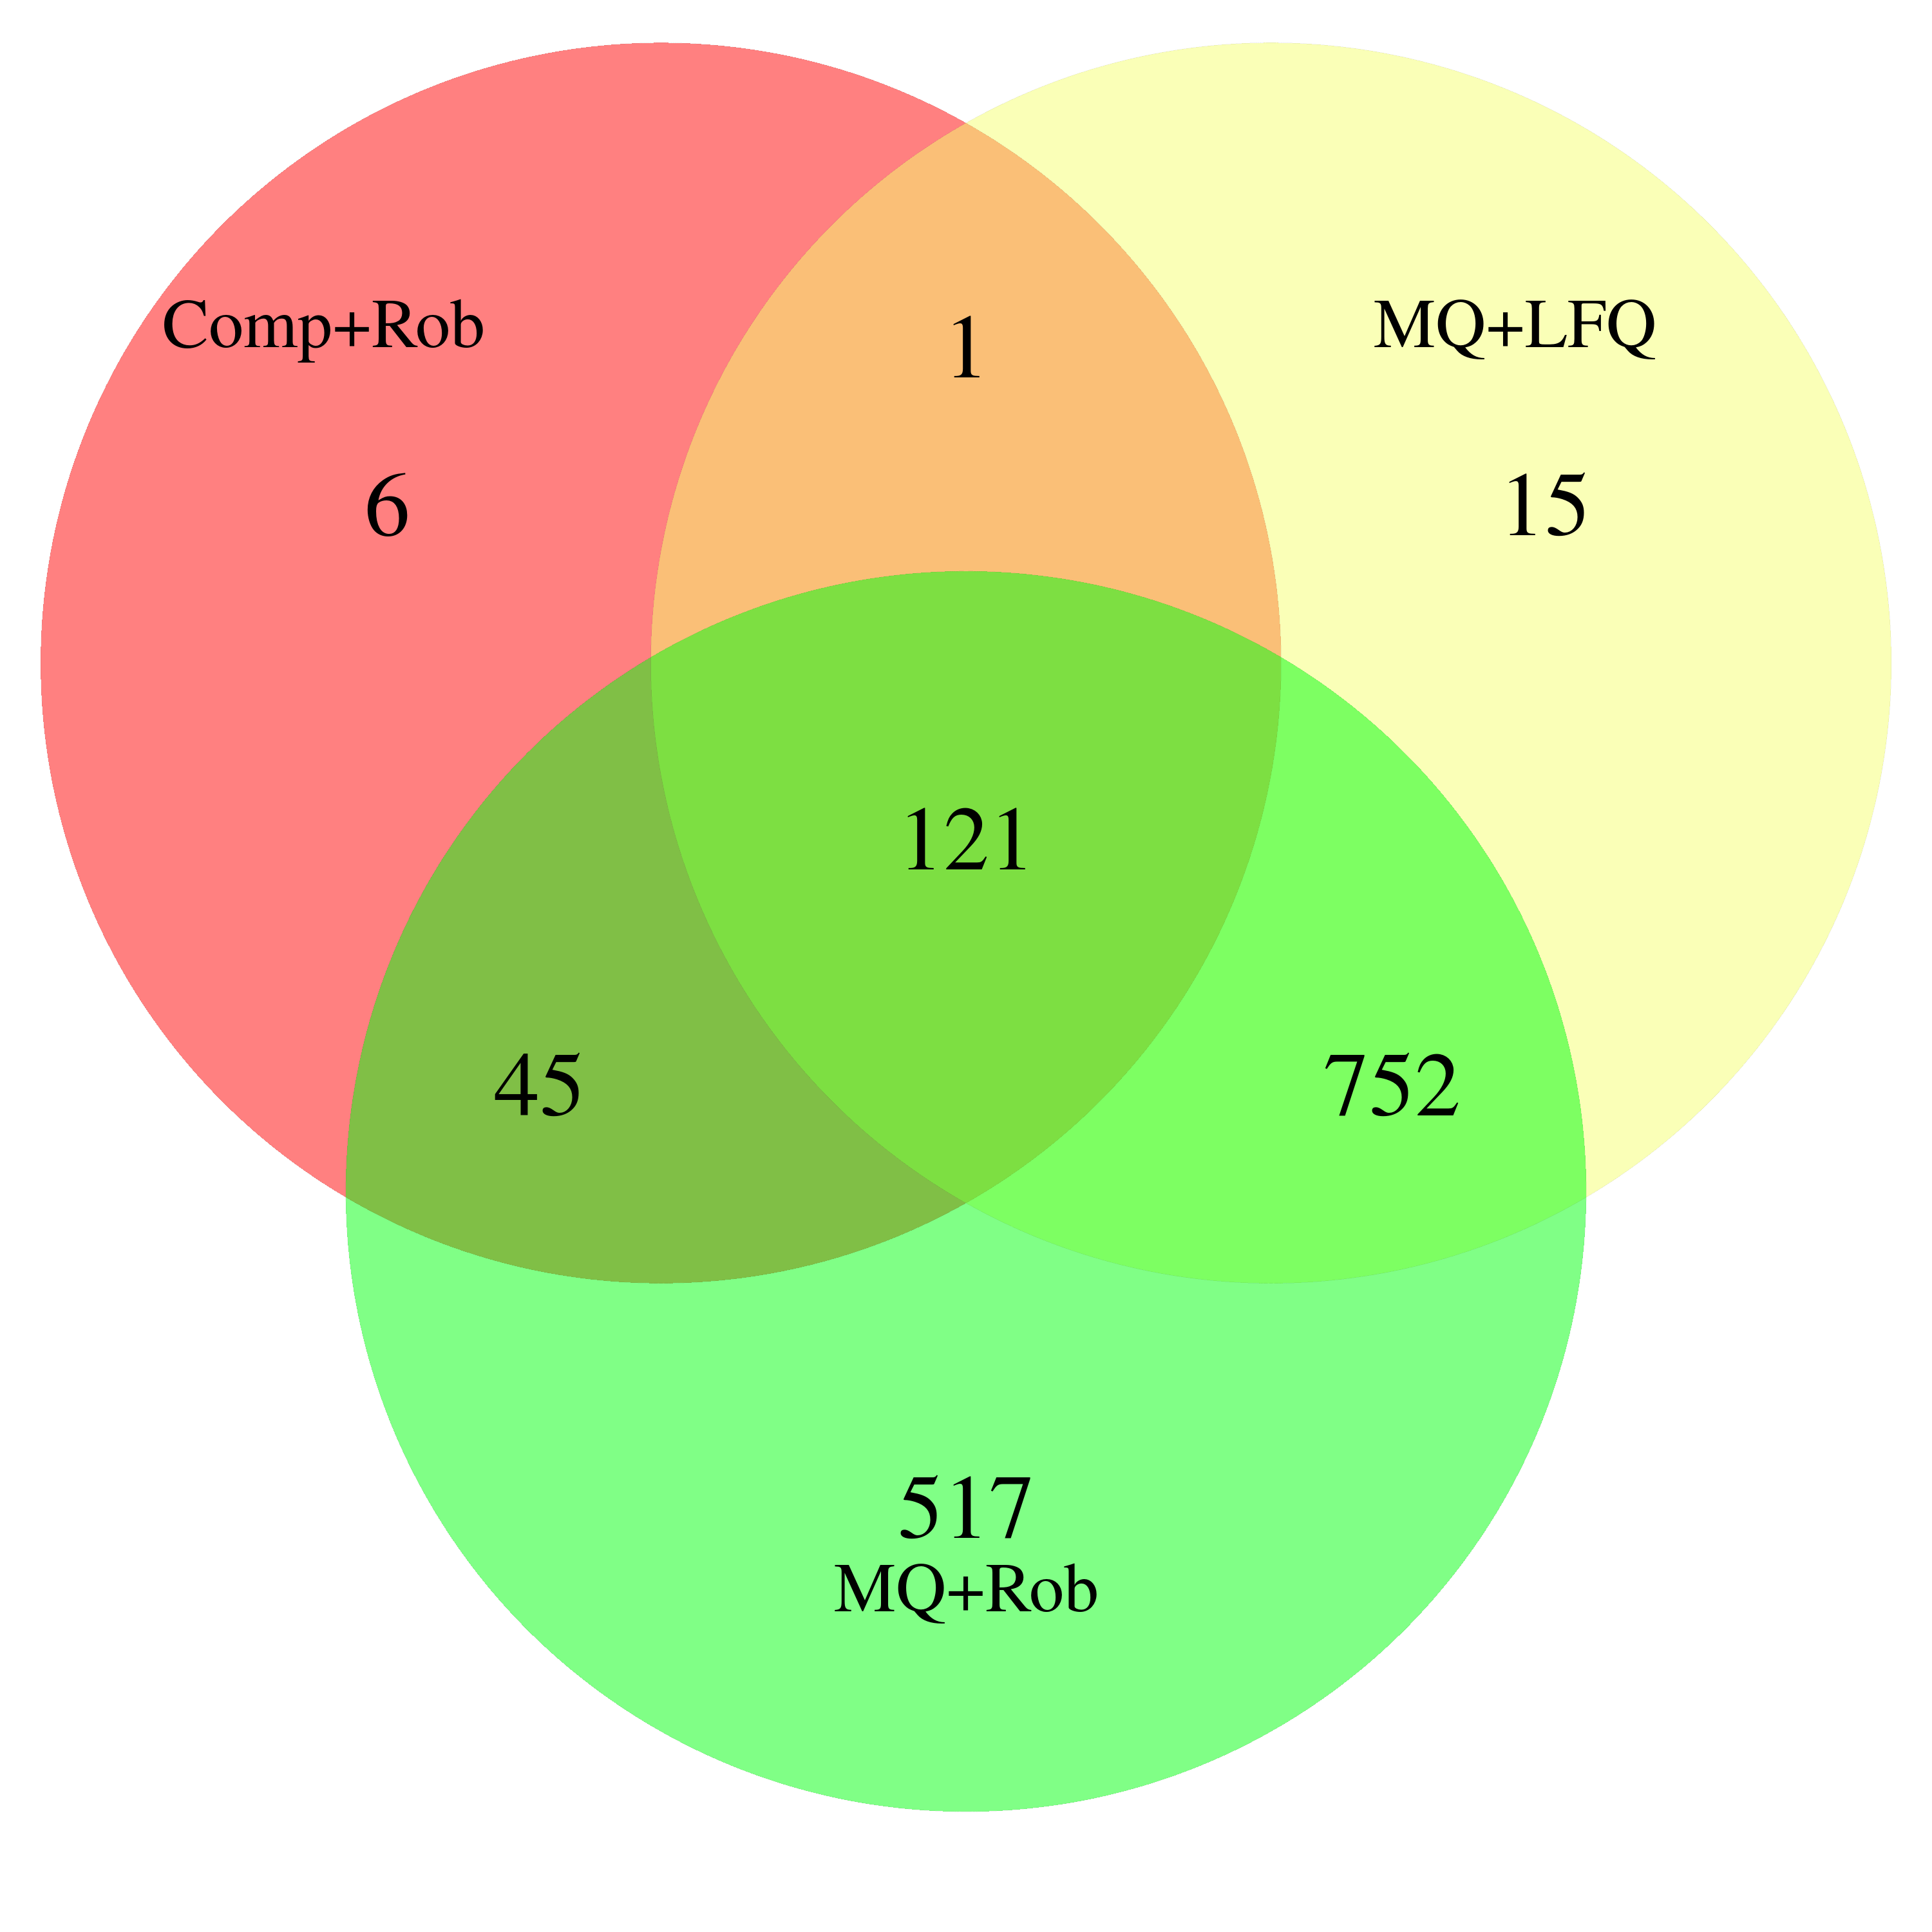
\includegraphics[width=.9\textwidth]{vennDiagram}
\end{subfigure}
\begin{subfigure}{.52\textwidth}
\caption*{B}
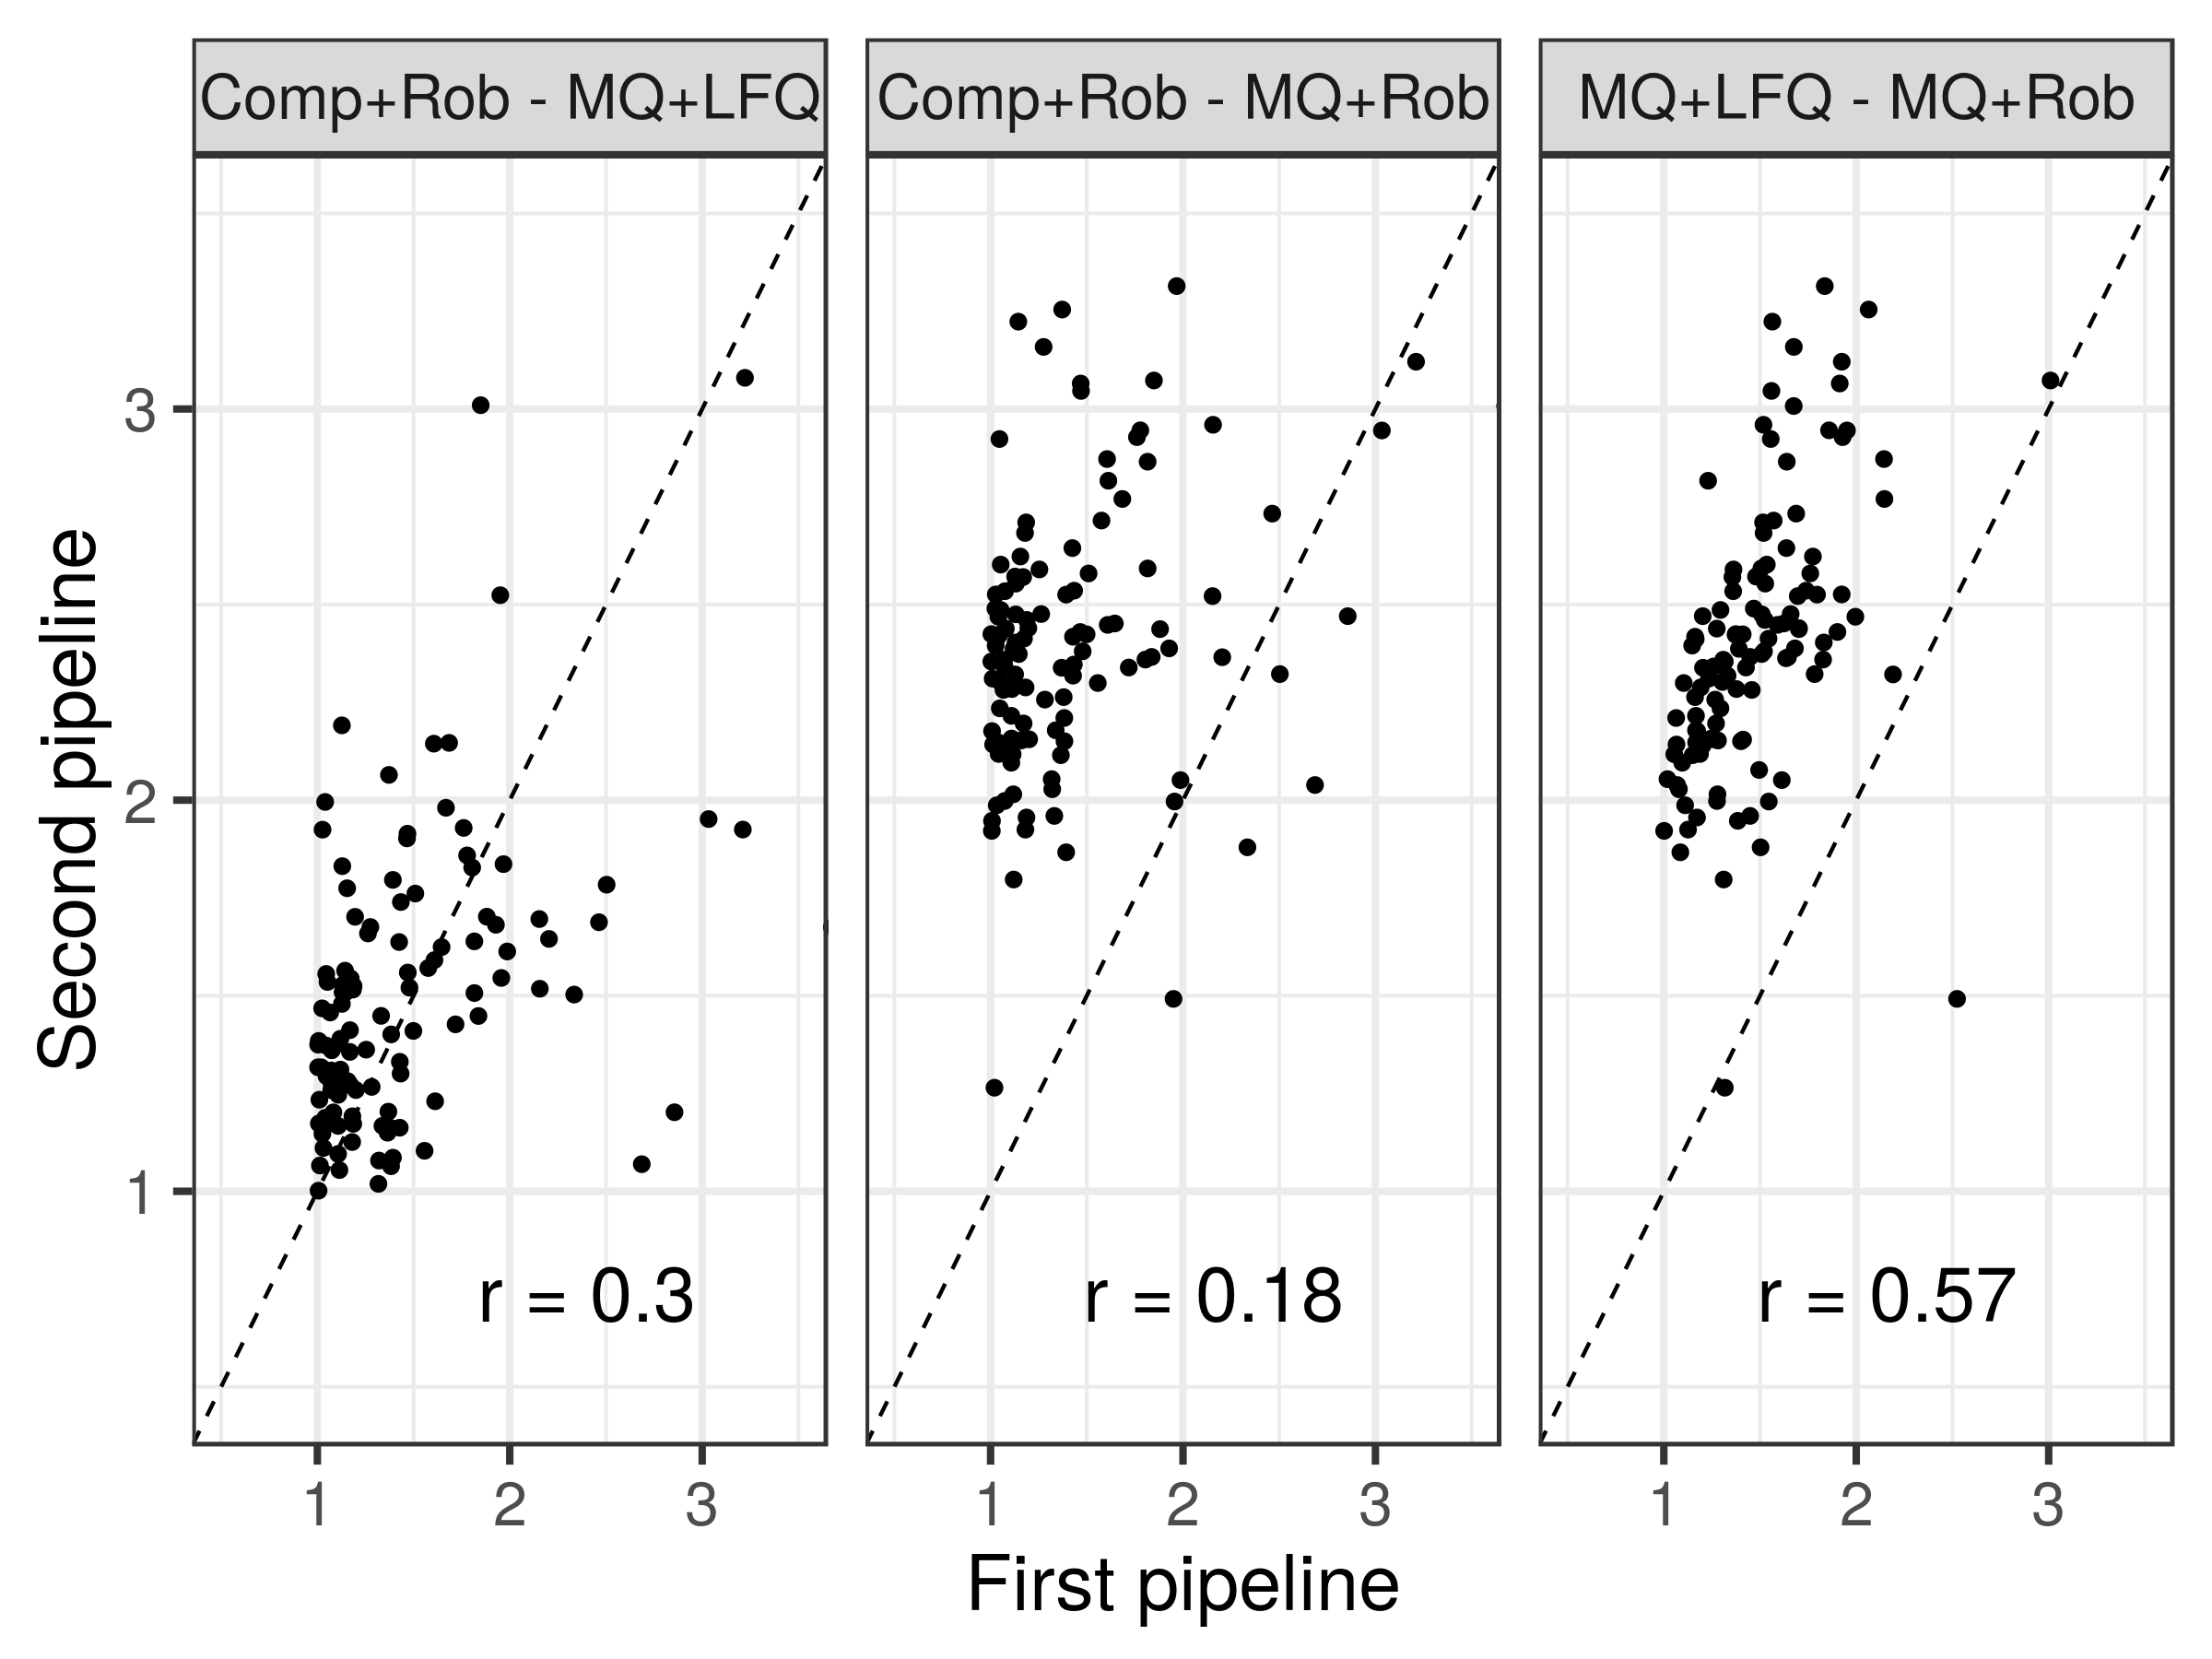
\includegraphics[width=.95\textwidth]{correlation_plot}
\end{subfigure}
\caption[Pipeline agreement plots]{Agreement between the different pipelines. \textbf{A} The Venn diagram displays the number of \textit{E. coli} proteins found to be differentially abundant by each pipeline. \textbf{B} The \ac{log2FC} estimated in all three pipelines for the 121 shared proteins is plotted by pairs to evaluate their correlation.}
\label{fig:venn_cor}
\end{figure}


In order to visualize the level of agreement of the pipelines for the assignment of differentially abundant proteins, a Venn diagram was constructed (see figure \ref{fig:venn_cor} A). Venn diagrams provide a straightforward visualization of the overlap of several ensembles of proteins. The scrutiny of the counts reveals a high degree of agreement, with most proteins detected by Comp+Rob or MQ+LFQ being detected by MQ+Rob too. Remarkably, 517 proteins were detected by MQ+Rob alone, showcasing its resolving power. Analyzing the log2FC pairwise-correlation (see figure \ref{fig:venn_cor} B) reveals that the highest correlation was found between pipelines using MaxQuant as upstream spectra processor, as expected. Even though the observed correlation was low, the estimated log2FC was always greater than 1. The MQ+Rob pipeline systematically estimated \ac{log2FC} values greater than the other 2.


Additionally, the accuracy with which each program assigns a \ac{log2FC} estimate to each protein group, and how significantly different from the null value of 0 it was found to be, provides further insights on the pros and cons of each pipeline.

Two separate distributions were distinguished for each organism, with the most overlap being  observed in the Comp+Rob pipeline. Remarkably, a ratio of 1 (\ac{log2FC} of 0) was frequently assigned by MSqRob (see figure \ref{fig:combined_plot} A). The significance acquired by \textit{E. coli} proteins was highest in the MQ+Rob pipeline. This analysis confirmed that the pipeline providing the best separation between organisms was MQ+Rob.


\begin{figure}[H]
\centering
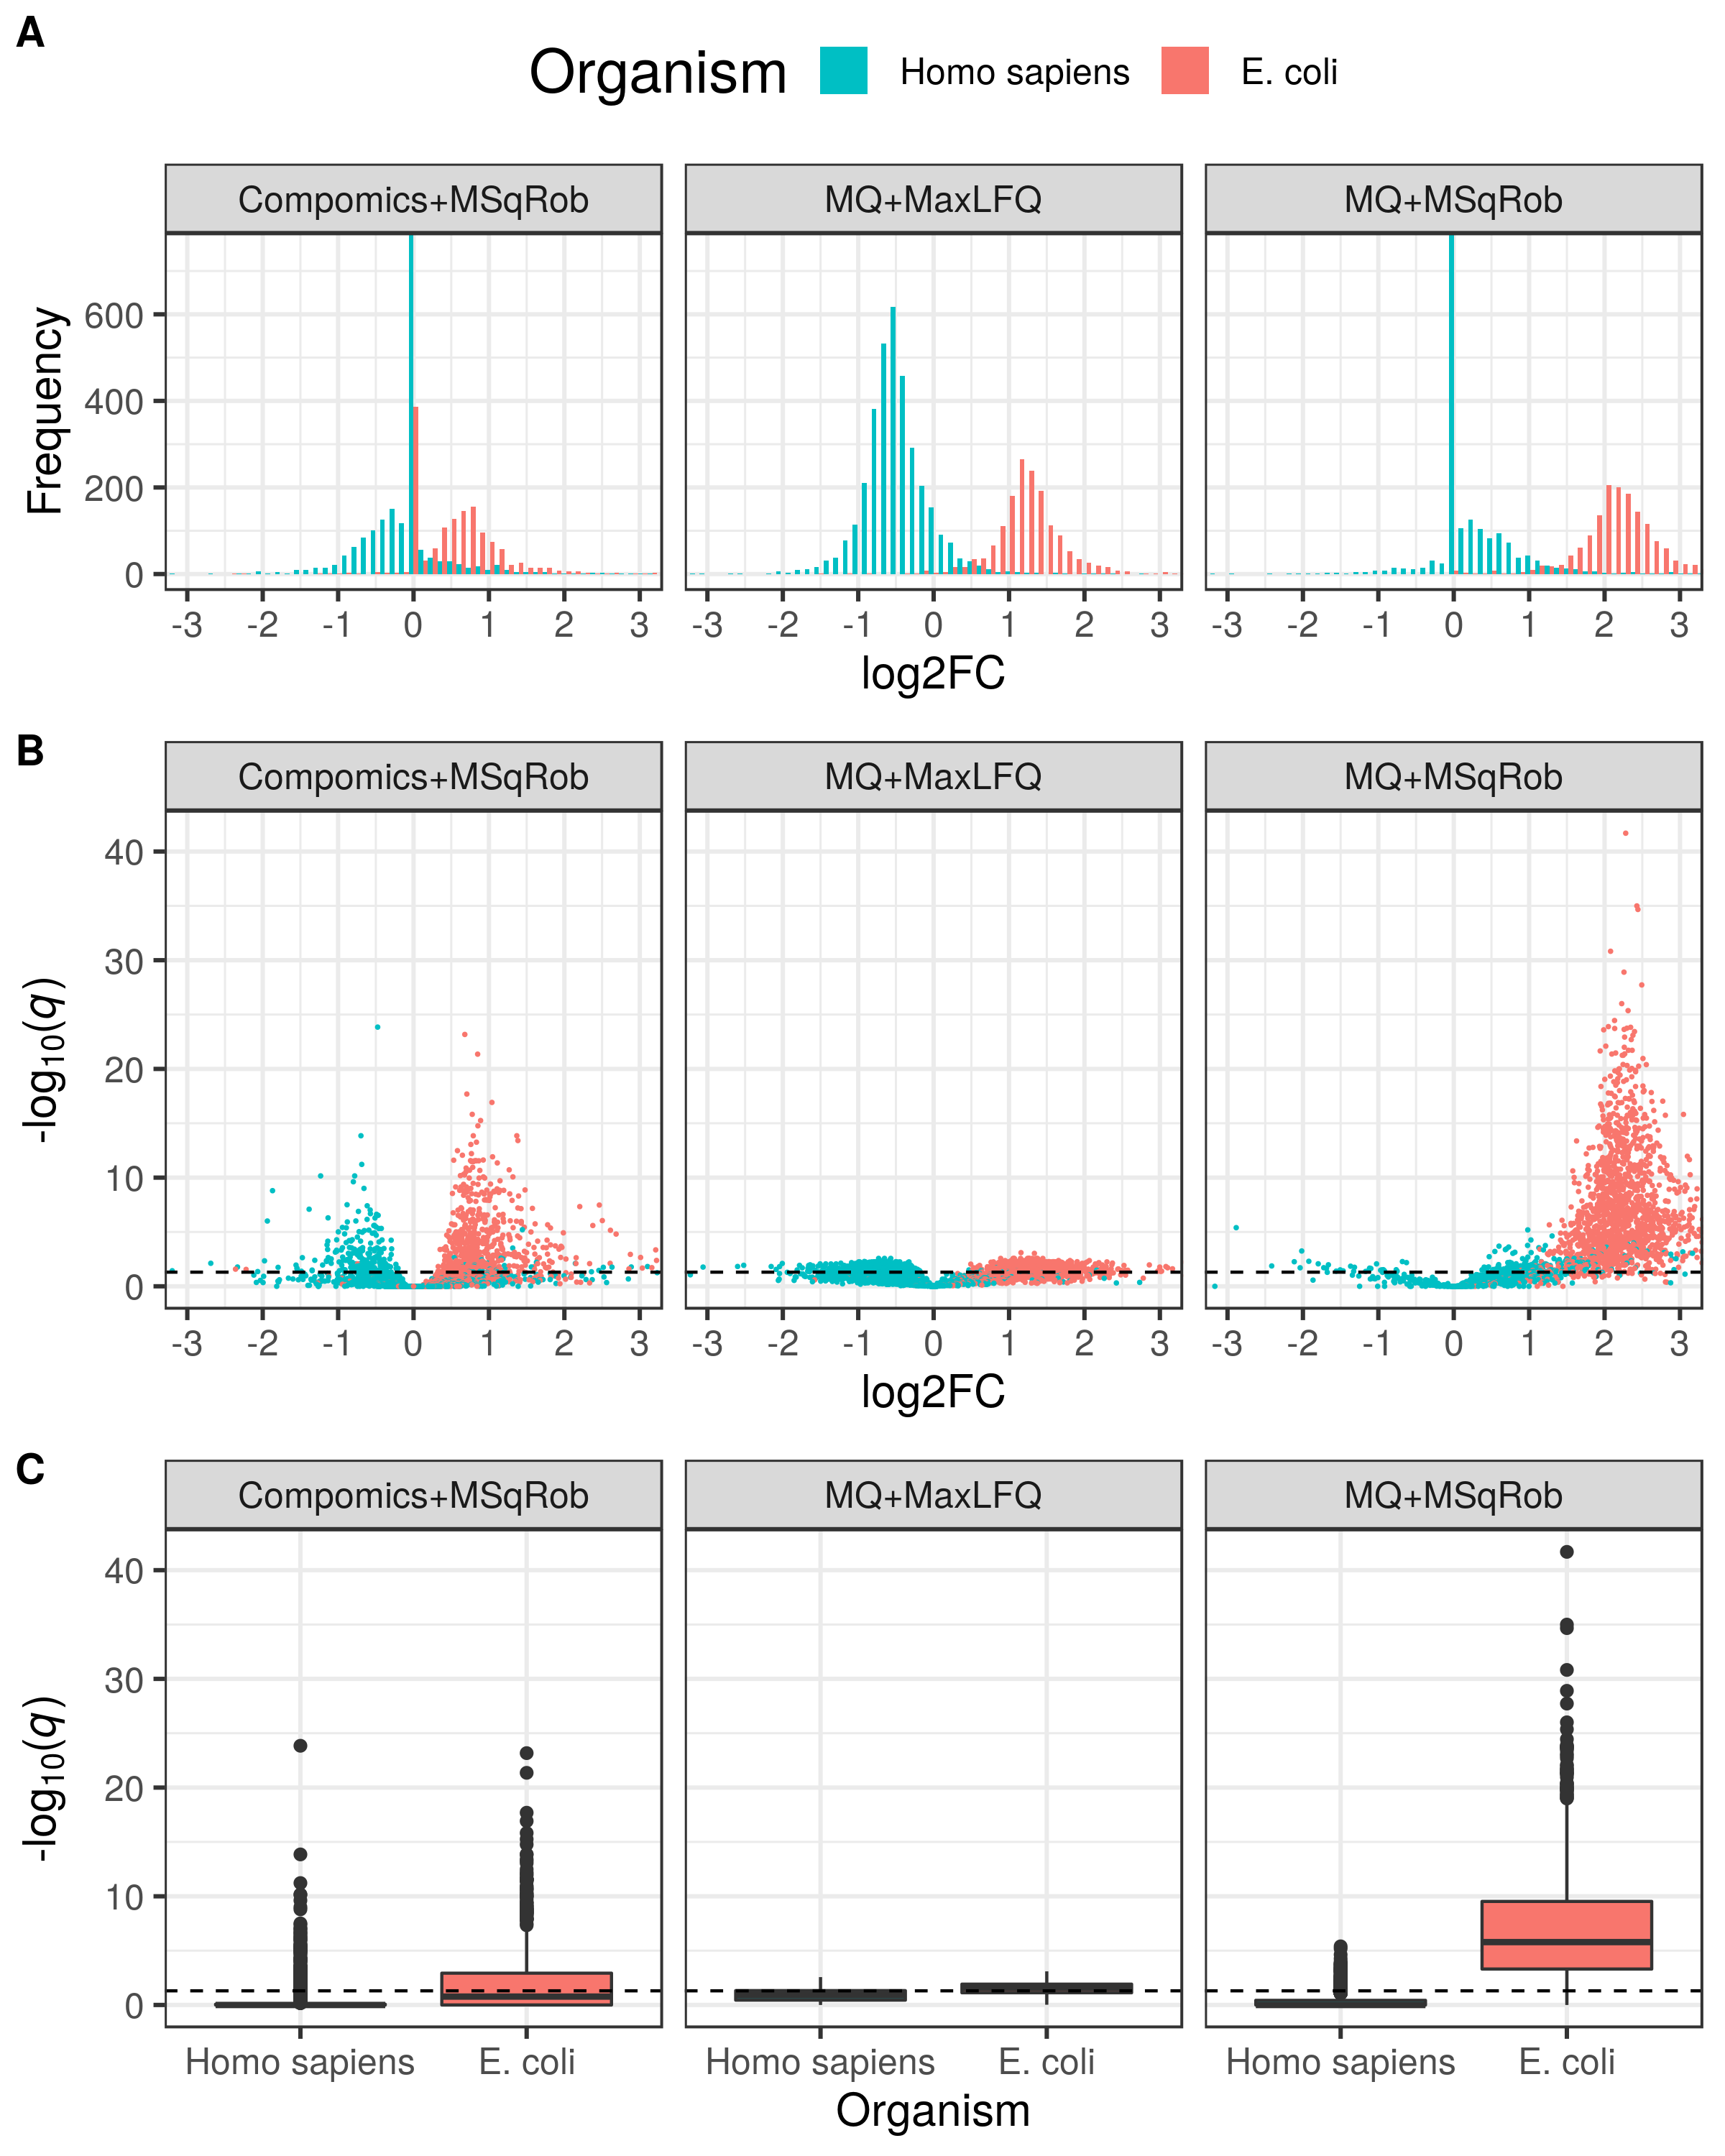
\includegraphics[width=\textwidth]{combined_plot}
\caption[Pipelines performance]{Overview over the different pipelines\textquotesingle performance. Quantification results are segregated by the source organism. \textbf{A} Histogram of the \ac{log2FC} estimates. \textbf{B} Volcano plot, where every protein group is represented by a dot and the coordinates map to its \ac{log2FC} on x and the minus logarithm of the q-value on y. \textbf{C} Boxplots of the minus logarithm of the q-value distribution.}
\label{fig:combined_plot}
\end{figure}



\section{Discussion}

\subsection{Improvement of the PSM step}

The low attained matching rate manifests existing room for improvement in the currently available tools. As explained in section \ref{sec:search_engines}, it has been shown that the combined usage of multiple search engines can increase identifications, since the different statistical frameworks implemented in each of them compensate each other\textquotesingle s caveats. Only MS-GF+ was used in this work for simplicity. Furthermore, \textit{de novo} search engines are available and supported by SearchGUI, and the latest developments in the field, like the IdentiPy engine \cite{Levitsky2018} are progressively incorporated to the tool \footnote{Issue on how to add IdentiPy\href{https://github.com/compomics/peptide-shaker/issues/309}{https://github.com/compomics/peptide-shaker/issues/309}}. Their usage is predicted to improve identification rates and quality of the matches.

A key reason on why many spectra remain unidentified is the presence of post-translational modifications (\ac{PTM}s), which exponentially increase the search space, forcing most workflows to discard many of the peptides featuring a PTM. New approaches to the problem are emerging, mainly machine learning methods for the handling of unexpected modifications \cite{Gabriels}. Moreover, the prediction of \ac{MS2} peak intensities patterns from peptide sequences promises to increase the amount of evidence available during the PSM process, thus boosting correct identifications \cite{Kirik2018} \cite{Degroeve2013}.

Finally, the extremely low matching rates in the latter fractions translated to decreased contributions to the number of identifications. This indicated that decreasing the number of fractions would not have had a major impact in the experiment\textquotesingle s depth.

\subsection{Improvement of the feature extraction step}

While the apex intensity is a good estimate of the peptide abundance, other methods are available that could potentially provide more robust data, such as the area of the peak. This is the approach taken by the recently published tool RawQuant \cite{Kovalchik2018}, or the feature detection tool in the OpenMS pipeline \cite{Sturm2008}. Moreover, in order to fine tune the performance of the \ac{MBR} and Apex intensity extraction steps, several input arguments can be adapted to each dataset. These are the spectrometer\textquotesingle s \ac{m/z} resolution, the time window used during the apex search and whether or not to activate outlier filtering and what weights to use.

\subsection{Improvement of the quantification step}

The deployed relative quantification approach successfully manages to estimate the \ac{log2FC} of several of proteins in the dataset with high confidence. However, it was not found to be the best performing of the assayed pipelines in the benchmark dataset. Several axes of improvement are clear from the results.

\subsubsection{Management of sample fractionation}

Sample fractionation allows for a deeper analysis of the peptide mix, which in turn leads to increased identifications and an increased amount of data to be analyzed. However, it simultaneously provides an extra random effect that hinders quantification if not handled properly.

The way the MaxLFQ engine solves the problem is by aggregating the data from the same sample across fractions using a weighted average. One normalizing weight is determined for every fraction via the \textit{Levenberg-Marquant minimisation of the overall proteome variation} $H(N)$ as defined in \cite{Cox2014}. A custom implementation was written in Python using the scipy module, but the results were not satisfactory. An issue regarding this is active on GitHub \footnote{\href{https://github.com/lgatto/MSnbase/issues/344}{https://github.com/lgatto/MSnbase/issues/344}}.

If fraction aggregation is not supported, MSqRob can be set to treat fractions as a random effect, as explained in section \ref{subsec:quantification}. However, if this is done, the statistical model in Comp+Rob can be overwhelmed by the inconsistency resulting from a 24-plex sample fractionation, leading to null \ac{log2FC} estimates for many \textit{E. coli} proteins. This is clearly manifested in figure \ref{fig:combined_plot} B, which shows many bacterial proteins were assigned  a \ac{log2FC} of 0, indicating MSqRob did not find enough evidence to discard the null hypothesis. While no \textit{E. coli} proteins fell in this category in the MQ+MSqRob pipeline, many did in the Comp+Rob, proving room for improvement in this aspect.

In any case, the way sample fractionation is handled should depend upon the fractionation method. For example, membrane fractionation can be exploited when working with membrane proteins \cite{Marmagne2006}.

To sum up, the presently implemented fraction handling is correct and provides good results, but fine-tuning of the pipeline at this step is expected to improve the results of the quantification. Thanks to the open-source nature of the software, this is indeed possible.


%which is defined according to the following expressions:
%
%\begin{equation}
%I_{P,A}(\text{N}) = \sum\limits_{j=1}^{k}{\text{N}_{A,j} \times \text{XIC}_{P,A,j}}
%\end{equation}
%
%where $\text{N}_{A,j}$ stands for the normalization coefficient for sample $A$ and fraction $j$, and $\text{XIC}_{P,A,j}$ stands for the extracted ion current in the same sample and fraction for peptide P. The sum runs over all k fractions.
%
%\begin{equation}
%H_P(N) = \sum\limits_{A,B} \abs{\log(\frac{I_{P,A}(N)}{I_{P,B}(N)})}^2
%\end{equation}
%
%\begin{equation}
%H(N) = \sum\limits_{p} H_p(N) 
%\end{equation}
%
%where the pair $A$ and $B$ is any of the sample pairs where peptide $P$ is detected. The overall proteome variation is 


\subsubsection{The pitfalls of mass spectrometry}

The application of mass spectrometry to proteomics is a very hot topic in research, driving innovations in the way the different components of the spectrometer work. One recent example is the development of the timsTOF\texttrademark\xspace Pro (Trapped Ion Mobility Spectrometry-Time Of Flight) system by Bruker, which supports PASEF (Parallel Accumulation and SErial Fragmentation) spectrometry \footnote{\href{https://www.prnewswire.com/news-releases/bruker-launches-the-timstof-pro-mass-spectrometer-to-enable-the-revolutionary-pasef-method-for-next-generation-proteomics-300520791.html}{Press release of the PASEF Method https://www.prnewswire.com/news-releases/bruker-launches-the-timstof-pro-mass-spectrometer-to-enable-the-revolutionary-pasef-method-for-next-generation-proteomics-300520791.html}}. This technology adds  an extra dimension peptide separation process, leading to cleaner spectra.
Notwithstanding, the developments also reveal the immature state of the technology. Slight inconsistencies in the protein extraction and digestion, bias in the peptide ionization, presence of unexpected PTMs, and detector saturation and insensitivity, remain as problems contributing to the eventual measurement variability characteristic of mass spectrometry \cite{Piehowski2013}. Thus, adequate preprocessing of the peptide dataset, and care to ignore outliers is preeminent. Indeed, the input file for the MQ+LFQ consisted of a preprocessed file which removed the most problematic proteins \cite{Cox2014}, which explains why more than 500 extra proteins could be quantified when using MSqRob (see figure \ref{fig:venn_cor} A).

\subsubsection{Support for absolute quantification}

While relative quantification like that performed by MSqRob is enough to infer differential abundance of proteins across conditions, absolute quantification would provide an estimate of protein quantities that would support many other analyses, and facilitate comparison between datasets, in a way similar to what the normalised read counts in FPKM (Fragments Per Kilobase per Million Reads) does in transcriptomics. On the other hand, MaxLFQ provides absolute estimates, albeit less robust.

\subsubsection{Quantification of uncertainty}

All the quantification approaches enunciated until now make use of different frequentist approaches to the problem, that evaluate how significantly different the data are from what would be expected under a null hypothesis of a null ratio across the pair of conditions. Yet, it does not provide probabilistic interpretations of the uncertainty behind the estimate. The development of a Bayesian framework which endeavors at solving this issue is presented in chapter \ref{chap:model}.

\subsection{Applicability for Novozymes data}

The SearchGUI and PeptideShaker developers recommend using Uniprot-formatted databases for optimal performance of their tools \footnote{\href{https://github.com/compomics/searchgui/wiki/DatabaseHelp}{Database formatting guide https://github.com/compomics/searchgui/wiki/DatabaseHelp}}. This is due to the software making use of protein annotations to improve the protein inference step. In any case, a consistent formatting in the FASTA databases is required to use the tools. Thus, the development of sequence databases featuring consistent FASTA identifiers is highly advisable to make the best use of the data and improve the interplay with not just these but many other tools too.


\section{Conclusion}

An open-source, cost-free, platform-agnostic and customizable label-free relative quantification pipeline assembling publicly available tools was presented in this work. The pipeline is capable of providing qualitative information on the protein composition of a sample using the latest proteomics search engines and validation software. Moreover, it can be extended to support more complex tasks, like \textit{de novo} search, or the study of \ac{PTM}s, thanks to its non-monolithic nature and usage of open-formats. Likewise, the openness of the data in all steps allows for quality control checks along the way. However, the comparison against other workflows shows the room for improvement in the quantification step when dealing with fractioned data, albeit deficiencies in this aspect should have no impact in non-fractioned datasets.

Either the pipeline developed in the presented chapter or those based on MaxQuant are ready to be deployed in a real environment and provide \ac{NZ} with useful insights on its proteomics data for free.
\chapter{BayesQuant: Probabilistic estimation of protein ratios}
\label{chap:model}

\section*{Summary}

The current label-free quantification methods, reviewed in section \ref{sec:quantification}, rely on frequentist statistics, which return point estimates of model parameters such as the abundance ratio (fold change) across conditions. However, a Bayesian  approach to this problem, that we know of, is lacking in the literature. As a response to this shortcoming, a statistical model, named BayesQuant, was written in the probabilistic programming framework PyMC3 and tested on the same benchmark dataset from chapter \ref{chap:pipeline}). The execution of the three steps required when doing Bayesian modelling, mainly (I) model implementation, (II) computation of posterior probabilities and (III) model checking, will be described for this particular problem in the present chapter, together with a discussion on its usability, its strengths and its weaknesses.

\section{Introduction}

\subsection{Frequentist and Bayesian statistics}

Both the LFQ and MSqRob quantification engines presented in chapter \ref{chap:pipeline} took a frequentist approach to the problem of protein quantification. Such approaches, establish a null hypothesis $H_0$, complementary to the actual hypothesis being tested (alternative hypothesis $H_1$). The information about the phenomena being modelled is put to use to measure how likely this null hypothesis is via Null-Hypothesis Significance Testing (\ac{NHST}).


\begin{align}
H_0: & \log_2(FC) = 0 \nonumber \\
H_1: & \log_2(FC) \neq 0 \nonumber
\end{align}

The results of this analysis will depend not only of the observed data, but also the data generation process \cite{Kruschke}. This way, both tools return point estimates of the \ac{log2FC} between a pair of conditions, and a p-value, which measures the probability of the null hypothesis. The null hypothesis usually states that the true value of the parameter is 0. Thus, p-values do not say anything about the probability of hypotheses outside $H_0$ and $H_1$.

The Bayesian statistical framework provides an alternative point of view by revolving the role played by the model parameters and the observed data. While frequentist statistics treats the data as random and the parameters as fixed, a Bayesian framework swaps their roles and yields a probability distribution for any model parameter given the provided data. Bayesian analyses rely on the observed data and prior knowledge about the phenomenon only, and come equipped with an equation that mathematically formalizes how to introduce these two dependencies in a valid way. This is the so called Bayes\textquotesingle s theorem.

\begin{equation}
P(\theta | y) = \cfrac{P(y | \theta) P(\theta)}{P(y)}
\end{equation}

The Bayes theorem is an extremely versatile tool taking a role analogous to that of statistics like T, F, or $\chi^2$. Unlike them, which are tailored to specific scenarios, it can be used to compute the probability distribution of almost any parameter in any model. 4 terms can be distinguished in its expression

\begin{enumerate}

\item $P(\theta)$: the \textbf{prior} probability distribution of the model parameter, introduces previous knowledge about the phenomenon being modelled.

\item $P(y | \theta)$: the probability distribution of the observed data (y) over the possible parameter space. It is also known as \textbf{likelihood} of the model, and its duty is updating our beliefs about the phenomenon by capturing the information in the data.

\item $P(y)$: the probability of the data, defined as the marginal probability of the data given a parameter value, for all possible values. It acts as a normalizing constant that makes the resulting distribution a true probability distribution adding up to 1. It is also known as the data \textbf{evidence}.

\item $P(\theta | y)$: the updated probability distribution of the model parameter, with the information extracted from the observed data. Since it reflects the beliefs about the phenomena after observing data, it is called \textbf{posterior} probability distribution, as opposite to the prior.

\end{enumerate}


The Bayes\textquotesingle s theorem formulated above is thus read as \textit{the posterior probability of the parameter $\theta$ is equal to the \textbf{prior} probability distribution times the likelihood divided by a constant}.

It can be applied to the quantification problem, where $\theta$ turns into the \ac{log2FC} parameter we try to estimate. All is needed is the computation of the posterior probability distribution. Unfortunately, this is tractable analytically for simple models only. However, Markov Chain-Monte Carlo (\ac{MCMC}) and Variational Inference (\ac{VI}) methods can be used to approximate this posterior. Both of which are now possible to run thanks to the advent of modern computing.

\subsection{Inference methods: \ac{MCMC} and \ac{VI}}

The posterior distribution can be approximated (inferred) by means of \ac{MCMC} and \ac{VI} methods. On the one hand, \ac{MCMC} methods simulate sampling from the posterior distribution by constructing an ergodic Markov chain on $\theta$ whose stationary distribution is the posterior p($\theta$ | y) \cite{Blei2017}. Monte Carlo sampling is performed on the Markov Chain, (hence the name of the technique) to randomly explore the parameter space with some heuristics. The heuristics guarantee convergence of the empirical estimate on the true posterior, provided a big enough sample size. Sampling convergence is defined as the status reached by the sampler when it estimates a distribution of probability that does not change anymore, regardless of how much longer the sampler runs \cite{Tran2018} \footnote{\href{http://www.cs.jhu.edu/~jason/tutorials/variational.html}{http://www.cs.jhu.edu/~jason/tutorials/variational.html}}. The first sampling algorithms, like Metropolis-Hastings \cite{Chib1995} \footnote{A very nice tutorial on the Metropolis-Hastings algorithm \href{http://twiecki.github.io/blog/2015/11/10/mcmc-sampling/}{http://twiecki.github.io/blog/2015/11/10/mcmc-sampling/}} have given way to the much more efficient sampler \ac{NUTS} \footnote{Likewise, this resource provides very illustrative explanations of Hamiltonian-MC and NUTS \href{http://elevanth.org/blog/2017/11/28/build-a-better-markov-chain/}{http://elevanth.org/blog/2017/11/28/build-a-better-markov-chain/}} \cite{Hoffman2011}.

On the other hand, \ac{VI} methods, very recently developed and introduced in PyMC3, provide a fast alternative to \ac{MCMC} methods, yet they are not guaranteed to asymptotically approximate the true posterior. In \ac{VI}, optimization, instead of sampling, is employed as the way to approximate the posterior \cite{Blei2017}. More concretely, a family of densities $Q$ over the parameters $\theta$ is defined. The goal of \ac{VI} is to find the single density $q$ within the family $Q$ that best approximates $p(\theta|y)$. This approximate density should be complex enough to reach a good approximation, and at the same time simple enough to be computationally easy to work with. The best candidate is defined as the one minimising the Kullback-Leibler (\ac{KL}) divergence (see equation \ref{eq:KL}).

\begin{gather}\label{eq:KL}
q^*(\theta) = \argmin \infdiv*{q(\theta)}{p(\theta|x)}
\end{gather}

where $q(\theta)$ stands for the whole family of densities, $p(\theta|x)$ stands for the true posterior and $KL$ stands for the \ac{KL} divergence. $q^*(\theta)$ is the best candidate density.

\textit{The term variational is used because the best $q$ in $Q$ is picked. The term derives from the "calculus of variations," which deals with optimization problems that pick} [...] \textit{a particular $q$ in $Q$, specified by setting some variational parameters i.e the knobs on $Q$ that need to be turned to get a good approximation}\footnote{\href{http://www.cs.jhu.edu/~jason/tutorials/variational.html}{http://www.cs.jhu.edu/~jason/tutorials/variational.html}}.


One of the terms yielded by the decomposition of the conditional density embodied by the posterior is the evidence of the data $p(x)$.  $p(x)$ is computationally intractable, thus making the computation of the exact \ac{KL} divergence impossible. A lower bound up to an additive constant can however be computed thanks to Jensen\textquotesingle s inequality \cite{jensen1906fonctions} \. This approximate amount is the Variational or Evidence Lower BOund (\ac{ELBO}). \textit{The \ac{ELBO} is the negative \ac{KL} divergence of plus $logp(x)$, which is a constant with respect to $q(z)$. Thus maximizing
the \ac{ELBO} is equivalent to minimizing the \ac{KL} divergence} \cite{Blei2017}.

Finally, several density approximation families are available. The mean-field family of densities is one of the most simple, as it ignores all dependencies between latent variables, and treats them as independent. The mean-field approximation works by \textit{pretending that the variables are just behaving that way "on their own." The mean-field method throws away all of the interactions}\footnote{\href{http://www.cs.jhu.edu/~jason/tutorials/variational.html}{http://www.cs.jhu.edu/~jason/tutorials/variational.html}}. A generic mean-field family member is shown in equation \ref{eq:mean_field}.

\begin{equation}\label{eq:mean_field}
q(\theta_1, ..., \theta_m) = \prod_{j=1}^{m}{q(\theta_j)}
\end{equation} 

The demanding computational cost of the \ac{MCMC} and \ac{VI} schemes has only been recently met by the power of modern computers, thus making the approach feasible.


\subsection{Hierarchical modelling}
\label{subsec:hierarchy}


The data recorded in this particular problem consist of \ac{MS1} intensities. They are affected by two main sources of variation:

\begin{enumerate}
\item The fixed effect that the researcher aims at unraveling with proteomics (treatment effect).
\item Random noise produced by experimental procedures, sequence bias, etc, which lead to a loss of data quality and resolving power.
\end{enumerate}


A mass spectrometry-proteomics workflow aims at providing estimates of the treatment effect, upon which the biological interpretation of the results is done, while minimising the remaining unwanted effects. A mathematical modelling of these effects (see equation \ref{eq:model}), similar to the one used by MSqRob, can be deployed to attempt to minimise the noise:

\begin{equation}\label{eq:model}
y_{ijkl} = \beta_{i}^{0} + \beta_{ij}^{treatment} + \beta_{ik}^{peptide} + \beta_{il}^{run} + \epsilon_{i}
\end{equation}

where $y_{ijkl}$ stands for the $\log_2$-transformed intensity registered in treatment $j$, peptide $k$ and run $l$. This way, separate treatment, peptide and run effects are distinguished. $i$ stands for the protein index, which is evidently the same for all measurements belonging to peptides mapped to the same protein. $\epsilon$ models the noise that cannot be explained with the three effects aforementioned, and is the same for all measurements associated to the same protein.

For example, the measurement $y_{P,A,p,1}$ corresponds to a measurement mapped to protein $P$. The measurement is impacted by a fixed effect, produced by treatment $A$, but also the peptide effect in peptide $p$ and the run effect in run $1$. An intercept term was also added to account for the background protein intensity value.

The data is thus said to be affected by different effects acting independently, and in order to model them properly, multi-levels need to be defined. It can be done via three approaches: pooled, unpooled, and hierarchically (see figure \ref{fig:multilevel}). Hierarchical modelling is used when the sampling variance is not the only source of variation among the parameters, but they still share a dependency. The intercept and the three effects were modelled as independent hierarchies.

\begin{figure}[!h]
\centering
\begin{subfigure}{.9\textwidth}
\centering
\caption*{Pooled}
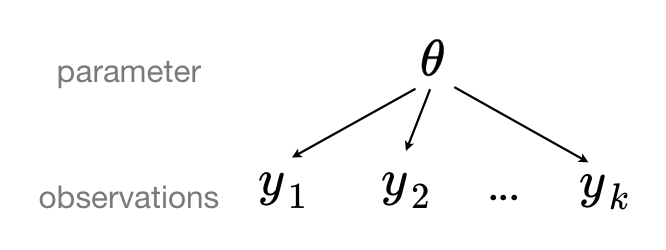
\includegraphics[width=0.85\linewidth]{model_pooled}
\end{subfigure}
\bigskip
\begin{subfigure}{.9\textwidth}
\centering
\caption*{Unpooled}
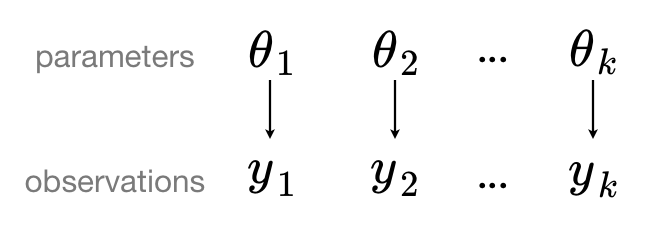
\includegraphics[width=0.85\linewidth]{model_unpooled}
\end{subfigure}
\bigskip
\begin{subfigure}{.9\textwidth}
\centering
\caption*{Hierarchical}
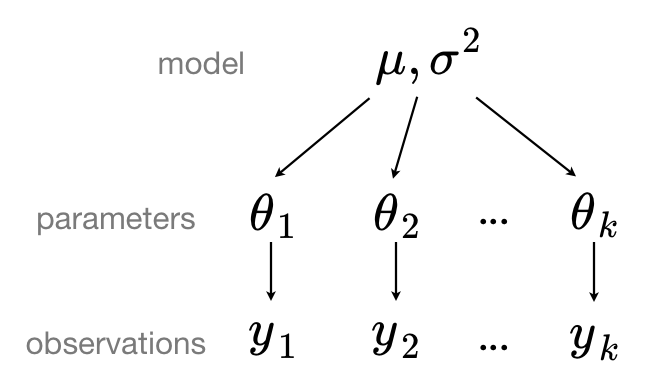
\includegraphics[width=0.85\linewidth]{model_hierarchical}
\end{subfigure}
\caption[]{Alternative multilevel modelling approaches. A pooled model assumes that the parameter distribution is the same for all the datapoints.  The unpooled model represents the opposite case, every datapoint is modelled by a different probability distribution. Finally, a hierarchical model settles for a middle ground where the parameters will not be exactly the same but not completely different either. This is achieved by generating a global distribution from which the parameter for each datapoint is sampled \footnotemark{}.}
\label{fig:multilevel}
\end{figure}
\footnotetext{\href{https://docs.pymc.io/notebooks/multilevel\_modeling.html}{https://docs.pymc.io/notebooks/multilevel\_modeling.html}}


This way, independent and identically distributed (\ac{IID}) priors were set for the intercept, treatment, peptide and run effects. The particular effect observed on each peptide was then modelled as a value sampled from the corresponding \ac{IID} prior. A diagram of the resulting model is displayed in figure \ref{fig:daft_model}.

\begin{figure}[!h]
\centering
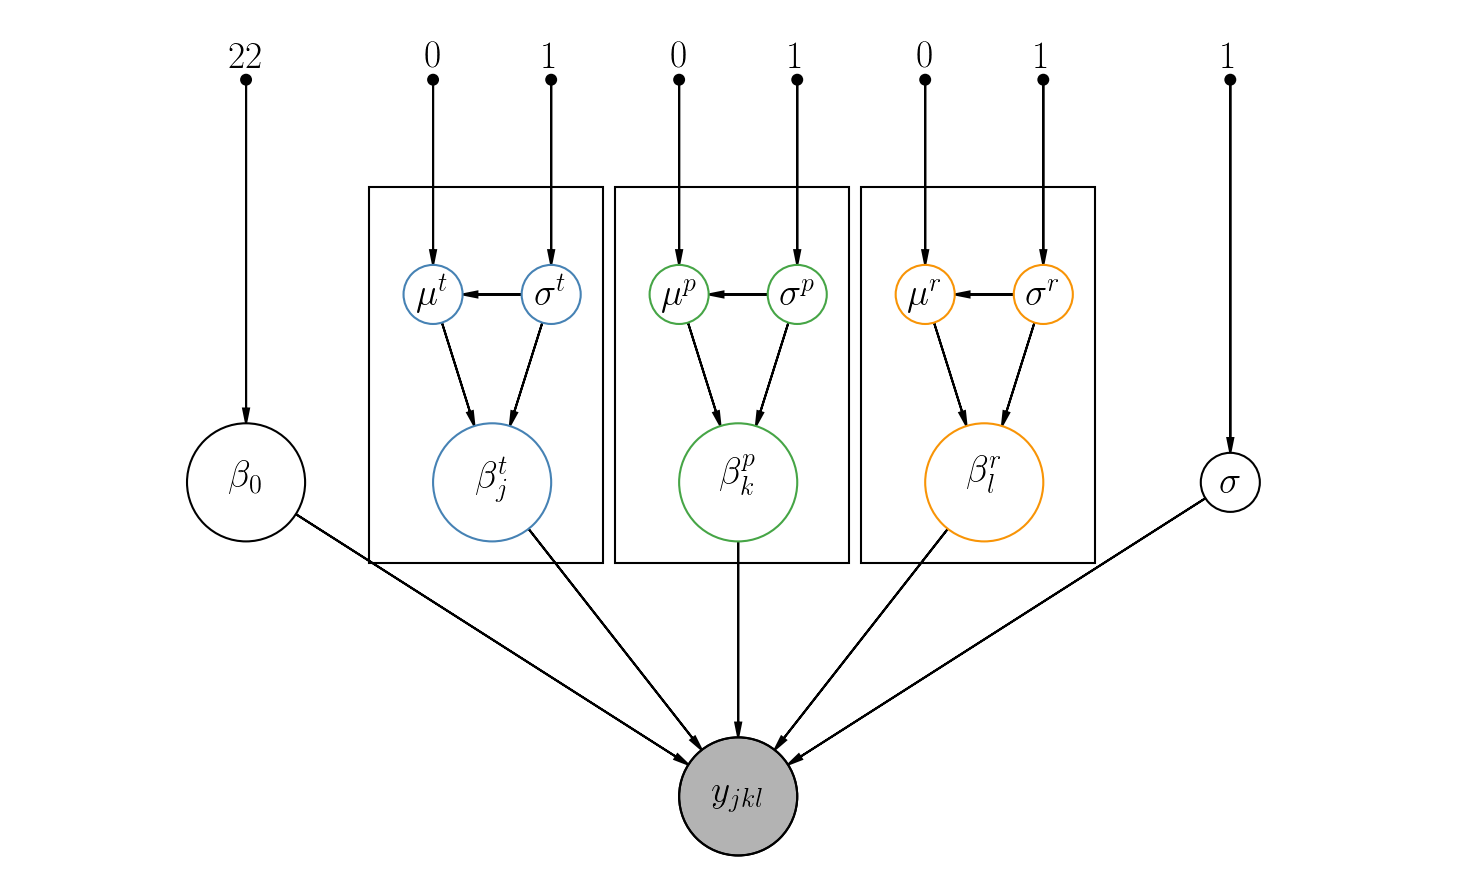
\includegraphics[width=\textwidth]{graph}
\caption[Bayesian model simplified diagram]{Diagram of the Bayesian model developed in the present work. It is represented as a Directed Acyclic Graph (\ac{DAG}) where nodes represent hyperparameters or random variables (in a circle) and directed edges  represent the dependencies between them. The nodes on the top depict the hyperparameters of the model, governing the prior probability distributions represented by the nodes to which their edges lead to. The remaining nodes articulate the probabilistic model and all lead to a final node ($y_{ijkl}$) which represents the modelling of the observed data with the instantiated model. The model hierarchies are organized in boxes. The one corresponding to the treatment effect can be read as \textit{the treatment effect $\beta_{ij}^{t}$ observed in the data is modelled as a probability distribution conditional on the value of $\mu^t$ and $\sigma^t$, which are in turn probability distributions governed by the hyperparameters 0 and 1.}}
\label{fig:daft_model}
\end{figure}

\subsection{Model checking}
\label{subsec:model_checking}

However the posterior distribution is obtained, a proper Bayesian analysis is not finished without a model checking step that looks at potential problems happening in the fitting step, and confirms the goodness of fit of the model to the data.

\begin{itemize}

\item Evidence for non-convergence must be collected. Albeit lack of evidence of non-convergence does not guarantee convergence, the existence of evidence definitely proofs it \cite{Kruschke}.

\item Neither reaching convergence nor the best \ac{VI} approximation guarantee that the fitted model actually captures the data generation process. Therefore, the true posterior could be a bad reflection of the natural process being modelled and the best approximation will not fix it. Posterior Predictive Checks are carried out to measure how well the model captured the data properties \cite{Kruschke}.

\end{itemize}




\subsection{Probabilistic programming}

The infrastructure providing the inference and model checking algorithms is available under several implementations in different programming languages, like R (JAGS \cite{Plummer}) and Python (PyMC3 \cite{Salvatier2016}). All these frameworks make use of a programming paradigm called \textbf{probabilistic programming}.


The management of uncertainty in statistics is done by means of probability distributions, which account for the possible values that a parameter could take, together with how likely they are. Probabilistic programming offers the framework to build complex statistical models by storing probability distributions as variables of the program. Moreover, probabilistic programming packages supply the tools needed to perform inference with these models by taking experimental evidence (data) and fitting the distributions to the data using Bayes\textquotesingle theorem.

%The fit of the model to the data entails the computation of the posterior probability distribution, which is tallied using algorithms provided with the probabilistic programming tool.

PyMC3 is a mature Python module dedicated to support probabilistic programming. It features   intuitive model specification syntax, modern and powerful \ac{MCMC} sampling algorithms like the No-U-Turn-Sampler (\ac{NUTS}) as well as Automatic Differentiation Variational Inference (ADVI) \footnote{\href{https://github.com/pymc-devs/pymc3}{https://github.com/pymc-devs/pymc3}}. Therefore, it provides the tools required to build a Bayesian model for the probabilistic estimation of protein \ac{log2FC} in proteomics datasets, that is, together with an estimate of its uncertainty.


\subsection{Goals}

\begin{enumerate}

\item Develop a Bayesian model to estimate log2FC in proteomics datasets together with the uncertainty of the estimate.

\item Make it scalable and fast for usability in ordinary modern computers.

\end{enumerate}

\section{Materials and Methods}

\subsection{Data input}
\label{subsec:data_input}

The peptides.txt and proteinGroups.txt files produced by MaxQuant \cite{Cox2008} after the analysis of the dataset published in \cite{Cox2014} were used as input for the modelling algorithm when running without sequence modelling, and processed using the \texttt{preprocess\_MaxQuant()} and \texttt{MSnSet2protdata()} functions in the MSqRob \cite{Goeminne2016} package, similar to what was done in section \ref{subsec:database_preparation}.

Peptides missing in any of the samples available were dropped from the analysis.

The final state of the data is shown in table \ref{tab:data_model} for two different proteins.

\begin{table}
\begin{tabular}{llrrrrrr}
\toprule
protein &      Organism &     H1 &     H2 &     H3 &     L1 &     L2 &     L3 \\
\midrule
 P0A8I8 &       E. coli &  25.13 &  25.24 &  24.39 &  21.71 &  22.67 &  22.40 \\
 P0A8I8 &       E. coli &  21.49 &  23.10 &  23.38 &  21.34 &  22.65 &  21.25 \\
 P0A8I8 &       E. coli &  24.10 &  24.54 &  23.81 &  19.88 &  20.87 &  20.30 \\
 A6NDG6 &  Homo sapiens &  25.08 &  24.98 &  23.83 &  22.54 &  22.52 &  24.96 \\
 A6NDG6 &  Homo sapiens &  22.70 &  24.32 &  23.00 &  22.29 &  23.27 &  23.91 \\
 A6NDG6 &  Homo sapiens &  21.18 &  22.51 &  23.25 &  22.30 &  21.75 &  23.61 \\
\bottomrule
\end{tabular}
\caption[BayesQuant data input]{Sample data input for the Bayesian model. Every row represents a unique peptide. The first column refers to the protein it was found to map to in the protein inference step. The second column is an annotation field, in this case indicating the protein\textquotesingle s organism. The remaining columns indicate the $log_2(Intensity)$ registered for each peptide in the corresponding run. In this case, three peptides were observed for the proteins with ids \textit{P0A8I8} and \textit{A6NDG6}.}
\label{tab:data_model}
\end{table}

\subsection{Sequence feature extraction}

When running with active sequence modelling, the peptide sequences were extracted from \textit{E. coli} and \textit{Homo sapiens} proteome databases (\ref{subsec:database_preparation}).
%The protein neighborhood was defined by a window spanning 15 aminoacids on both sides of the peptide. It was extracted using the seqinr \cite{Charif2007} and GenomicRanges \cite{Lawrence2013} packages implemented in R and Bioconductor.

Features to model the peptide effect based on sequence were extracted using the Biopython \cite{Cock2009} built-in  module \texttt{ProtParam.ProteinAnalysis()}. The following properties were extracted: amino-acid percentage, peptide length, molecular weight, mass/length ratio, isoelectric point, aromaticity and instability.


\subsection{Prior probability distribution specification}

Both because of the little knowledge on the value of the parameters governing the data generation process and to provide a prior that everyone can agree upon, non informative priors were provided to the model. This was condensed in the specification of Normal and Half Normal distributions for all the random stochastic variables in the model. The hyperparameters were selected to be as non informative as possible.

\subsection{Posterior probability distribution computation}
\label{subsec:posterior_compute}

The \ac{VI} mean-field strategy was applied to approximate the posterior probability distribution of the \ac{log2FC}. \ac{ELBO} optimisation was run for 40k iterations. Optimisation was validated by visual inspection of \ac{ELBO} traceplots. Once optimisation was validated, 10k samples were drawn from the approximate distribution to simulate the true posterior.

\subsection{Model checking}

Posterior predictive checks of the posterior distribution were carried out using the \texttt{sample\_ppc()} function in PyMC3. 500 datapoints for each peptide, consisting of 6 numbers, one for each run, were simulated. The resulting 6D data was projected onto a 2D plane via Principal Component Analysis. The covariance matrix required was computed on the whole dataset. The visual evaluation of the differences between simulated and observed data was used to assert the correctness of the models.

\subsection{PyMC3}

In order to get started with PyMC3, we first need to import it.

\begin{minted}[mathescape,
               linenos,
               numbersep=5pt,
               autogobble=true,
               frame=lines,
               framesep=2mm]{python}


import pymc3 as pm              
\end{minted}

The model is initialized as a Python context manager. Within the context manager, the model is implemented by defining prior distributions for the model parameters and establishing the dependency relationships between them.

A PyMC3 implementation of the priors set on the bias in \ac{MS1} intensity measurements due to a random effect is shown here.

\begin{minted}[mathescape,
               linenos,
               numbersep=5pt,
               obeytabs=true,tabsize=2,
               firstnumber=last,
               frame=lines,
               framesep=2mm]{python}

with pm.Model() as model:             
         sigma = pm.HalfNormal('sigma', 1)
         mu = pm.Normal('mu', mu=0, sd=sigma)
\end{minted}


Which is equivalent to the following statistical notation:

\begin{align}
\sigma \sim \mathcal{HN}(1)\,.  \\
\mu \sim \mathcal{N}(0,\,\sigma)\,.
\end{align}

and can be read as \textit{the prior probability distribution of the random effect follows a normal distribution with mean 0 and standard deviation $\sigma$. In turn, $\sigma$\textquotesingle s prior probability distribution follows a half normal distribution with standard deviation 1}. 1 and 0 act as hyperparameters of the model, and introduce the state of beliefs or knowledge on the system prior to seeing the data.


The hierarchical structure of the model is set by the definition of a parameter distribution from which the value for each element (peptide) being modelled is sampled. This can be done by defining a new normal distribution where its $\mu$ and $\sigma$ are set to the random variables defined above. In PyMC3 code,

\begin{minted}[mathescape,
               linenos,
               numbersep=5pt,
               obeytabs=true,tabsize=2,
               firstnumber=last,
               frame=lines,
               framesep=2mm]{python}
         beta = pm.Normal("beta", mu, sigma, n_elements)  
\end{minted}

which is equivalent to:

\begin{equation}
\beta^e_i \sim \mathcal{N}(\mu, \sigma)\,.  \\
\end{equation}

and can be read as \textit{the probability distribution of the bias observed in the $i^{th}$ element due to the effect here modelled is said to follow a normal distribution with mean $\mu$ and standard deviation $\sigma$ both defined as random probability distributions above.}

Finally, the equation \ref{eq:model} defined above closes the model and binds the data to the model parameters. Its PyMC3 implementation is the following:

\begin{minted}[mathescape,
               linenos,
               numbersep=5pt,
               obeytabs=true,tabsize=2,
               firstnumber=last,
               frame=lines,
               framesep=2mm]{python}
               
         epsilon = pm.HalfNormal('epsilon', 1)                
         m = pm.Deterministic("m", beta)
         obs = pm.Normal("obs", m, epsilon, observed=y)
      
\end{minted}

which is equivalent to

\begin{align}
\nonumber \epsilon \sim \mathcal{HN}(1) \,. \\ 
m = \sum_{i=1} \beta_i \,. \\ 
\nonumber y \sim \mathcal{N}(m, \epsilon)
\end{align}

and is read as \textit{the observed data is modelled by a normal distribution with mean $m$ and standard deviation $\epsilon$. $m$ is a random deterministic variable resulting from the sum the effects defined above. $\epsilon$ follows a new half normal distribution with standard deviation 1}. A deterministic variable is a random variable that acquires a fixed value if all random variables it has a dependency on take a fixed value too, i.e its stochasticity disappears if its parameters are fixed.




\section{Results}


\subsection{Running BayesQuant}

BayesQuant takes a peptide\_summary\_intensity\_moFF\_run.tab (moFF) or a peptides.txt file (MaxQuant) as input, containing a peptide per row. Preprocessing using the MSqRob \texttt{preprocess\_MSnSet()} function, as well as other data munging functions, is required.

%--peptide_file> <--filetype> <--exp_annotation> [--annotation_df] [--organisms] [--protein_file] [--extract_features]

\begin{minted}[mathescape,
               linenos,
               numbersep=5pt,
               obeytabs=true,tabsize=2,
               frame=lines,
               framesep=2mm]{R}

Rscript prepare_BayesQuant.R --pepf peptides.txt \
    --filetype MaxQuant --exp exp_annotation.tsv \
    --output .
\end{minted}

The R script outputs the input file for BayesQuant. Its data is introduced in BayesQuant via the following code:

\begin{minted}[mathescape,
               linenos,
               numbersep=5pt,
               obeytabs=true,tabsize=2,
               frame=lines,
               framesep=2mm]{python}

# Load the module
from BayesQuant import BayesQuant
bayesquant = BayesQuant()
# Read the dataset
bayesquant.read_data(data="ms1_intensities.tsv")
# Compile a model for proteins with 3 peptides
model = bayesquant.compile_model(n_peptides=3)
# Load a specific protein
bayesquant.load_data("A6NDG61")
\end{minted}

The snippet above loads the program, reads in the data, selects a specific protein, and builds a model that matches the number of peptides observed. The posterior distribution can be computed using pure MCMC or VI methods, as stated in section \ref{subsec:posterior_compute}. The VI procedure will now be explained, due to its significantly better performance in this particular problem.

\begin{minted}[mathescape,
               linenos,
               numbersep=5pt,
               obeytabs=true,tabsize=2,
               frame=lines,
               firstnumber=last,
               framesep=2mm]{python}
# VI approximation: much faster and accurate
trace_advi = bayesquant.fit(model_name=p, n_draws=40000)
\end{minted}

The \texttt{bayesquant.fit()} function carries out two tasks:

\begin{itemize}
\item Finds the best mean-field approximation $q(\theta)$ to the true posterior $p(\theta|x)$. This approximate distribution is easier to work with.
\item Sample from the approximate posterior, returning a collection of samples called trace.
\end{itemize}

The values stored in the trace obtained via VI will follow an approximation to the true posterior, and contain the results of the modelling process. Once it is obtained, the inference is complete and model checking ought to be performed to validate the results as explained in section \ref{subsec:model_checking}. It is run with:

\begin{minted}[mathescape,
               linenos,
               numbersep=5pt,
               obeytabs=true,tabsize=2,
               frame=lines,
               firstnumber=last,
               framesep=2mm]{python}
# Run Posterior Predictive Checks
bayesquant.ppc()
\end{minted}

A step by step exposition of the plots and results produced by the program when ran on the proteins  P0A818 (\textit{E. coli}) and A6NDG6 (\textit{Homo sapiens}) follows.

%\begin{figure}[H]
% \centering 
% 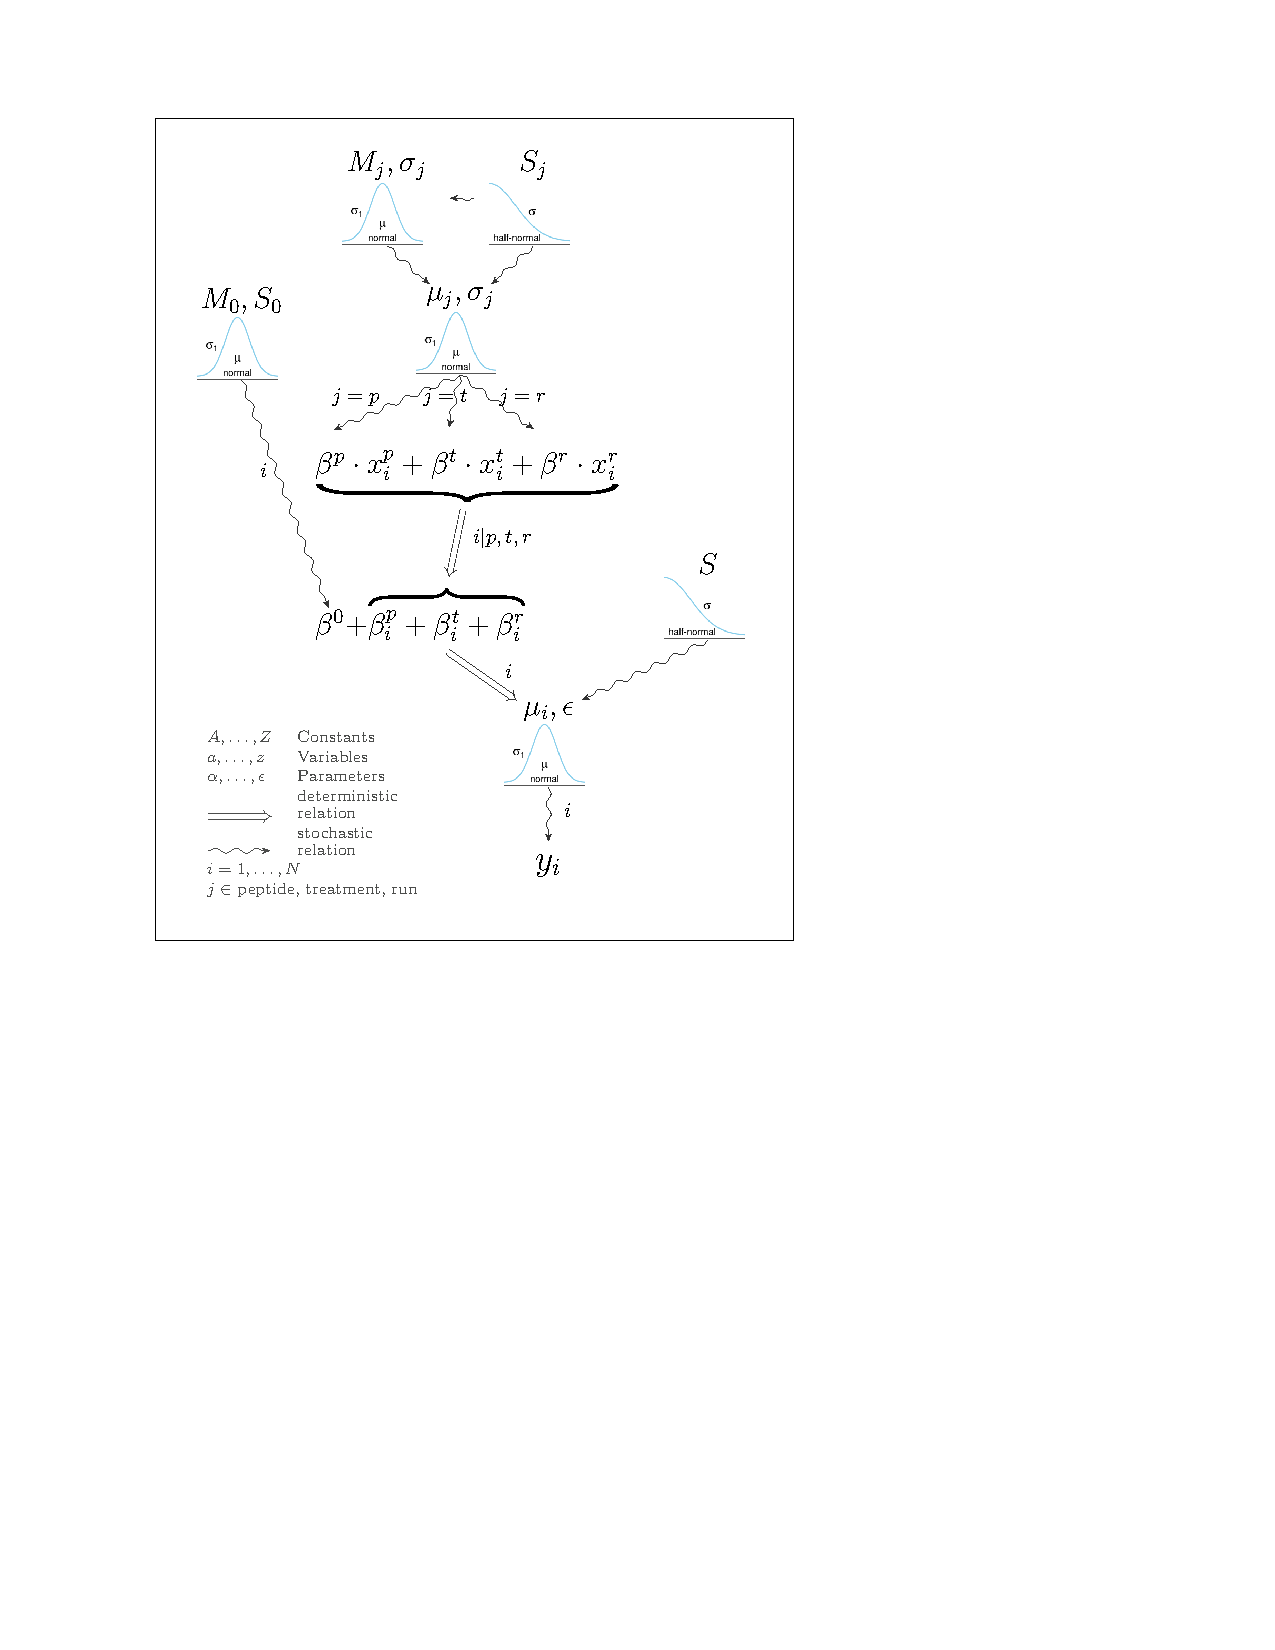
\includegraphics{hierarch_diagram.pdf}
% \caption{}
% label{fig:dbda}
%\end{figure}
\begin{figure}[!h]
% Hierarchical diagrams, DBDA
% ---------------------------------
% Tinu Schneider, October 2013


\documentclass[12pt]{article}

%\usepackage[T1]{fontenc} 
%\usepackage[utf8]{inputenc}

\usepackage[margin = 20mm, nohead, nofoot]{geometry} 

\usepackage{tikz}
    \usetikzlibrary{positioning, arrows, backgrounds, decorations, 
    				decorations.pathmorphing, decorations.markings, calc}
  
\graphicspath{{./distribution_diagrams/svg_without_names}}
    
\pagestyle{empty}

\usepackage{tgheros} 
\renewcommand*\familydefault{\sfdefault} 
	

% Macros for the distributions
% greek
\newcommand{\normalGreek}[1]{\greek{#1}{normal} } 
\newcommand{\gammaGreek}[1]{\greek{#1}{gamma} }
\newcommand{\halfnormalGreek}[1]{\greek{#1}{halfnormal} }   


\newcommand{\greek}[2]{\large$#1$\\ \includegraphics*[scale = 0.25]{distribution_diagrams/png_with_params/#2.png} }				 	 
   			
% letters (constants)  
\newcommand{\normalLetters}[1]{\letters{#1}{normal}} 
\newcommand{\gammaLetters} [1]{\letters{#1}{gamma}}   
\newcommand{\halfnormalLetters} [1]{\letters{#1}{halfnormal}}   



\newcommand{\letters}[2]{$#1$\\ \includegraphics*[scale = 0.25]{distribution_diagrams/png/#2.png} }

\usepackage{stackengine, scalerel}
\newcommand\Tunderbrace[3][]{%
  \def\tmp{#2}%
  \setbox0=\hbox{\tmp}%
  \stackunder[1pt]{%
    \stackunder[0pt]{\tmp}{\rotatebox{90}{\scaleto[2ex]{#1\{}{\wd0}}}%
  }{%
    \scriptsize #3%
  }%
}
\newcommand\Toverbrace[3][]{%
  \def\tmp{#2}%
  \setbox0=\hbox{\tmp}%
  \stackon[1pt]{%
    \stackon[0pt]{\tmp}{\rotatebox{90}{\scaleto[2ex]{#1\}}{\wd0}}}%
  }{%
    \scriptsize #3%
  }%
}

  						 	
   						 	
   						 	  						 	 
\begin{document} % ------------------------------ %

% distances
\def\smallY{0.25}
\def\midY{2.25}
\def\bigY{4.5}


\def\smallX{1.2}
\def\midX{1.5}
\def\bigX{2.7}


\begin{tikzpicture}[ framed, on grid,
   	node distance = \midY cm, 
   	inner frame xsep = 2.5ex,
   	inner frame ysep = 3.0ex,
    	box/.style = { rectangle,
	       		color = lightgray, 
	       		text = black,  
	       		text width = 2.0cm, 
	       		align = center},
	    boxFramed/.style = {box, 
	    		% draw, % uncomment this line, if you want the frames
	    		inner sep = 0pt},
	    boxFramedRound/.style = {boxFramed, rounded corners = 8pt},
	    boxFormula/.style = {box, inner sep = 1pt},
       	boxLegend/.style = {align = left, 
       			text width = 4cm, 
       			xshift = 2.2cm, 
       			yshift = 1.2cm,  
       			font = \scriptsize, 
       			color = black!70},
    	allArrows/.style = {font = \footnotesize, 
    			color = black!80, text = black},
    	arrSnake/.style = {allArrows, 
    			>=stealth', 
    			->, 
    			shorten >= 2pt, 
    			line join = round, 
    			decorate, 
  				decoration={snake, segment length = 10, 
  							amplitude = 1.2, post = lineto, 
  							post length = 4pt} },
     	implies/.style  = {allArrows, -implies, double, 
     			double equal sign distance, shorten >= 1pt}, 
     	labArrow/.style = {pos = 0.39},
     	labArrowLegend/.style = {labArrow, above, font = \tiny, inner sep = 3pt}
  	] 		   		
   		
   	% nodes for the distributions and equation(s)
   	% starting at the bottom				
	\node [box, xshift = 2cm] (yi) {\Large $y_{i}$};

   	\node [boxFramedRound, above = of yi, yshift = -.2cm] (final) {\normalGreek{\mu_{i}, \epsilon} } ;
   		   	
   	\node [boxFormula, above = of final, xshift=-\bigX cm, text width = 2.5 cm] (linMod)   
   			{ \large $\beta^0 +$\Toverbrace{$\beta^p_i + \beta^t_i + \beta^r_i$}{}} ;
   			
   			   	\node [boxFormula, above = of linMod, xshift= 0 cm, text width = 2.5 cm] (selectPar)   
   			{ \large \Tunderbrace{$\beta^p \cdot x^p_i + \beta^t \cdot x^t_i + \beta^r \cdot x^r_i$}{} } ;
    	
   	\node [boxFramed, above = of final,  xshift =  \bigX cm, yshift = \smallY cm] (proEpsilon) {\halfnormalGreek{S} } ;
    	
   	\node [boxFramedRound, above = of selectPar, yshift=.2cm, xshift = -\bigX-2.4 cm]   (proIntercept)   {\normalGreek{M_0, S_0} };
   	\node [boxFramedRound, above = of selectPar, yshift=\smallY cm, xshift = \smallX cm]   (proBeta)    {\normalGreek{\mu_j, \sigma_j} } ;
   	 
   	
   	\node [boxFramed, above = of proBeta,  xshift = -\smallX-1.2 cm] (promu)  {\normalGreek{M_j, \sigma_j} } ;
   	\node [boxFramed, above = of proBeta,  xshift =  \smallX+1.2 cm] (prosigma) {\halfnormalGreek{S_j} } ;        	
   	
   		    	
   		    	
   	% Arrows	    	
   	\draw[arrSnake] (final.south) --  node[right, labArrow] {$\ i$} (yi);
  	
    \draw[implies]  ($(linMod.south)+(1,-.15)$) -- node[right, labArrow] {$\ \ \ i$} (final.125);
    \draw[implies]  ($(selectPar.south)+(1.25,0)$) -- node[right, labArrow] {$\ i|p,t,r$} ($(linMod.100)+(1.1,0)$);


    \draw[arrSnake] (proEpsilon.south) -- (final.55);   
    
    \draw[arrSnake] (proIntercept.south) -- node[left, labArrow] {$\ \ i$} ($(linMod)+(-1,0)$);       	 	
    \draw[arrSnake] (proBeta.south) --  node[left,  labArrow] {$j=p\quad $} ($(selectPar)+(-1,.8)$);
    \draw[arrSnake] (proBeta.south) --  node[xshift=0cm,  labArrow] {$j=t\quad $} ($(selectPar)+(1,.8)$); 
    \draw[arrSnake] (proBeta.south) --  node[right,  labArrow] {$j=r\quad $} ($(selectPar)+(2.5,.8)$); 

            	
    
    \draw[arrSnake] (promu.south) -- (proBeta.122);       	 	
    \draw[arrSnake] (prosigma.south) -- (proBeta.57);  
    \draw[arrSnake] (prosigma.west) -- (promu.east);    	
  	
   	
   	
  	% Legend; needs improvement...
   	\node [boxLegend] at ( current bounding box.south west) (legendTitle) 
   		{%
   		\begin{tabular}{ll}
   			$A, \dots, Z$  & Constants \\
   			$a, \dots, z$ & Variables \\
   			$\alpha, \dots, \epsilon$ & Parameters \\ %[1ex]
   			
			 & deterministic \\[-0.4ex]
			 & relation \\ %[1ex]
			 
			 & stochastic \\[-0.4ex]
			 & relation \\ %[1ex]
			 
			\multicolumn{2}{l}{$i = 1, \dots, N$} \\
			\multicolumn{2}{l}{$j \in$ peptide, treatment, run} \\
			
   		\end{tabular}
   	};
   				
   	\def\xLegendArrowLeft{-3.75}
   	\def\xLegendArrowRight{-2.65}  
   	 	
   	\def\yLegendDouble{0.83}
   	\def\yLegendSnake{0.25}
   	
   	\draw[implies, black!70]  (\xLegendArrowLeft, \yLegendDouble) -- (\xLegendArrowRight, \yLegendDouble);    	   	
    \draw[arrSnake, black!70] (\xLegendArrowLeft, \yLegendSnake) -- (\xLegendArrowRight, \yLegendSnake);    	

\end{tikzpicture}

\end{document} % ------------------------------ %

\caption[BayesQuant Kruschke-like diagram]{\textbf{BayesQuant Kruschke-like diagram}. Extends figure \ref{fig:daft_model} to give more detail into the model. Prior probability distributions are indicated with "distrograms", and the dependencies between them via arrows. The hyperparameters are represented by latin capital letters.}
\label{fig:dbda}
\end{figure}

\subsection{VI optimisation evaluation}


\begin{figure}[H]
%\begin{adjustbox}{varwidth=\textwidth,fbox,center}
\begin{subfigure}{.45\textwidth}
\centering
\caption*{A}
\includegraphics[width=.9\linewidth]{ELBO/P0A8I8}
\end{subfigure}
\begin{subfigure}{.45\textwidth}
\centering
\caption*{B}
\includegraphics[width=.9\linewidth]{ELBO/A6NDG6}
\end{subfigure}
%\end{adjustbox}
\caption[ELBO progression]{Progression of \ac{ELBO} maximisation during the \ac{VI} approximation for proteins P0A818 (\textit{E. coli}, \textbf{A}) and A6NDG6 (\textit{Homo sapiens}, \textbf{B}) over 40k iterations.}
\label{fig:ELBO}
\end{figure}

A plot of the maximisation of the \ac{ELBO} is automatically produced when the texttt{.fit()} method is run. Even though the ELBO took extremely low (negative) values at start (see figure \ref{fig:ELBO}), it was maximised fast to values around 0, indicating that the mean-field approximation was acceptably good.


\subsection{Sampling from the approximation to the posterior}
\label{subsec:basic_model}


The 10k traces produced by BayesQuant from the \ac{VI} approximation function exhibited a clear random walk behaviour, which decreases the possibility that the approximation was wrong. Moreover, the  effects caused by the different peptides and runs were estimated and separated from the overall observed noise, allowing for a better estimation of the \ac{log2FC} (see figure \ref{fig:traceplots}).

\begin{figure}[!h]
%\begin{adjustbox}{varwidth=\textwidth,fbox,center}
\begin{subfigure}{\textwidth}
\centering
\caption*{A}
\includegraphics[width=\linewidth]{traceplots/P0A8I8}
\end{subfigure}
\bigskip
\begin{subfigure}{\textwidth}
\centering
\caption*{B}
\includegraphics[width=\linewidth]{traceplots/A6NDG6}
\end{subfigure}
%\end{adjustbox}
\caption[Traceplots for 2 proteins]{Traceplot of the model fit for proteins P0A818 (\textit{E. coli}, \textbf{A}) and A6NDG6 (\textit{Homo sapiens}, \textbf{B}). The left panel shows the frequency density over the parameter space for several model parameters: (I) the \ac{log2FC} estimate (difference of treatment effects), (II) the effects in the three observed peptides, and (III) the effects in the six available runs. The right panel displays the sampled values from the \ac{VI} approximation stored in the trace.}
\label{fig:traceplots}
\end{figure}

This way, a different posterior distribution was computed for the impact of each "peptide" and "run" in all the measurements collected for each protein.


The study of the \ac{log2FC} posterior probability distribution (see figure \ref{fig:posteriors}) shows the most likely parameter values and empowers Bayesian Null Hypothesis Testing. The 95\% High Probability Density Interval (\ac{HPDI}), which is the narrowest interval containing 95\% of the total probability, indicates the most likely true values of the parameter. Presence or absence of overlap between the 95\% \ac{HPDI} and the Region Of Practical Equivalence (\ac{ROPE}) provides a formal way of discarding a point value of the parameter. The \ac{ROPE} is a small interval considered to be essentially the same as the null value \cite{Kruschke}. In this and all future applications in the thesis, the null value is set to 0, and the \ac{ROPE} is arbitrarily set to $[-0.4, 0.4]$ based on the data.

\begin{figure}[!h]
\centering
\begin{subfigure}{0.8\textwidth}
\caption*{A}
\includegraphics[width=\linewidth]{posteriors/P0A8I8}
\end{subfigure}
\bigskip
\begin{subfigure}{0.8\textwidth}
\caption*{B}
\includegraphics[width=\linewidth]{posteriors/A6NDG6}
\end{subfigure}
\caption[Posteriors for 2 proteins]{Annotated posterior probability distribution for the \ac{log2FC} estimate for proteins P0A818 (\textit{E. coli}, \textbf{A}) and A6NDG6 (\textit{Homo sapiens}, \textbf{B}). The bar height is mapped to the probability mass in the corresponding interval. The 95\% \ac{HPDI} is marked with a black line. The \ac{ROPE} defined as a 0.4 window around 0 is shown in red. A green vertical line marks the expected \ac{log2FC} estimate for \textit{E. coli} proteins ($\log_2(3)=1.58$).}
\label{fig:posteriors}
\end{figure}

The analysis indicated that P0Q8I8 (\textit{E. coli}) most likely has a \ac{log2FC} between 1.4 and 1.7, and was found to be significantly different from 0, as no overlap was observed between the \ac{HPDI} and the\ac{ROPE}. On the other hand, the human protein was found to acquire a \ac{log2FC} most likely between -0.1 and 0.2. This range is fully contained within the \ac{ROPE}, which indicates that the \ac{log2FC} was practically 0 (see figure \ref{fig:posteriors}).


The posterior predictive checks on both proteins pinpoint that the fitted models captured a data generation process approximating what was observed (see figure \ref{fig:ppc}). The three observed peptides were found to be indistinguishable from the 500 simulated ones.

\begin{figure}[!h]
\centering
\begin{subfigure}{0.8\textwidth}
\caption*{A}
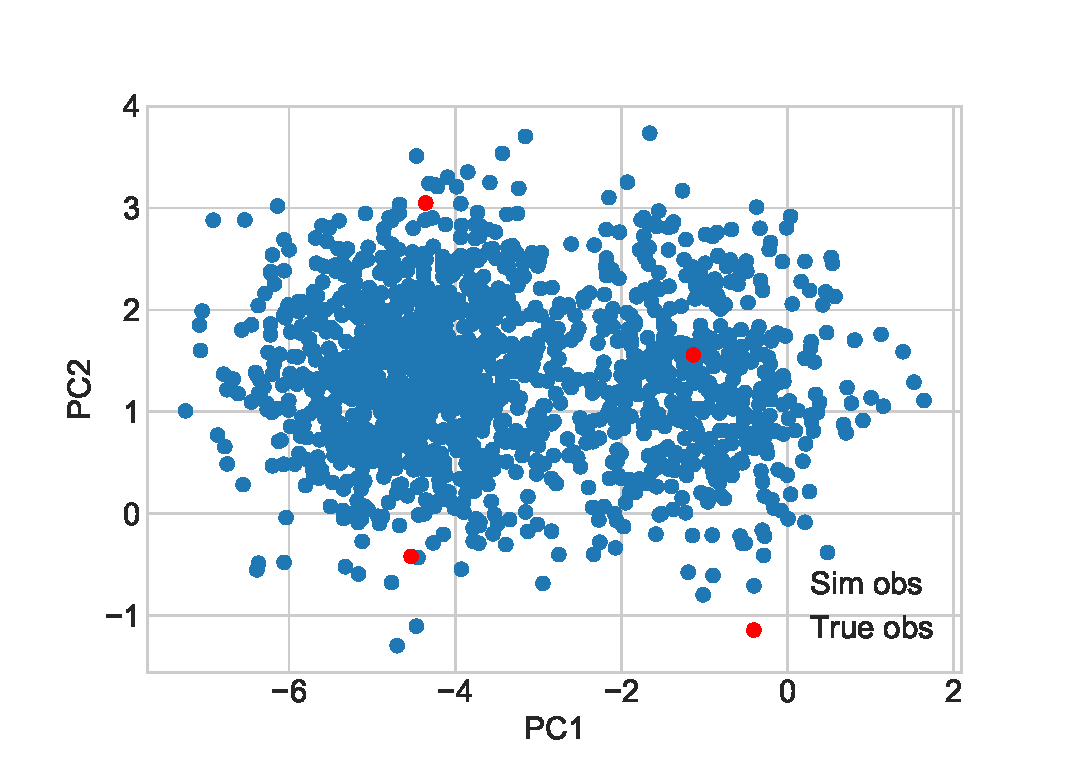
\includegraphics[width=\linewidth]{PPC/eps/PCA_P0A8I8}
\end{subfigure}
\bigskip
\begin{subfigure}{0.8\textwidth}
\caption*{B}
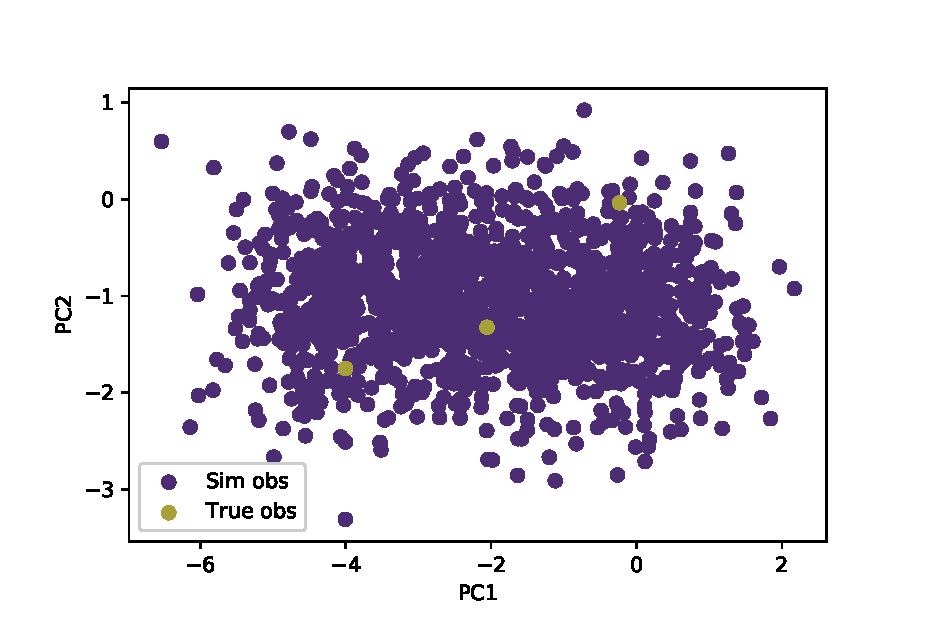
\includegraphics[width=\linewidth]{PPC/eps/PCA_A6NDG6}
\end{subfigure}
\caption[Posterior predictive checks]{Projection of the posterior predictive checks on the 2D plane capturing most variance. Simulated datapoints are shown in blue, whereas actual observations are shown on a clear color.}
\label{fig:ppc}
\end{figure}


In order to further validate BayesQuant\textquotesingle s performance, it was tested on groups of 5 proteins, one group from each proteome. Each pair of groups was made by proteins with a different number of observed peptides (2, 3, 4, 6, 7, 10) (see figure \ref{fig:dumbbell}). The more peptides, the more accurate the estimation will be as more data will be available. Since the \ac{HPDI} reflects the uncertainty, a decrease on its width was expected to be observed (see figure \ref{fig:dumbbell}).

\begin{figure}[!h]
\centering
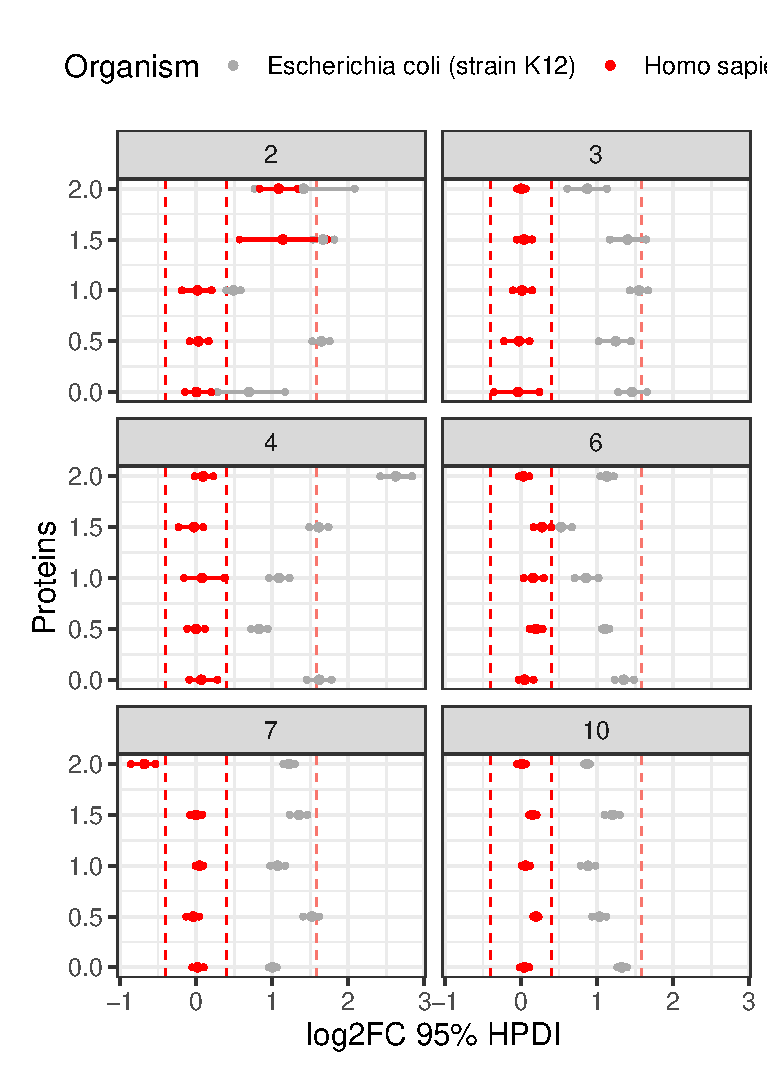
\includegraphics[width=0.9\textwidth]{performance}
\caption[HPDI inferred by BayesQuant]{Visualization of the 95\% \ac{HPDI} inferred from 5 bacterial and 5 human proteins with 2, 3, 4, 6, 7 and 10 peptides. The intervals are represented by horizontal lines. The dot represents the mean of the whole distribution, and it will be centered in the interval if the distribution is symmetrical. Vertical blue lines represent the ROPE defined as in figure \ref{fig:posteriors}, whereas the red line represents the expected estimate for bacterial proteins.}
\label{fig:dumbbell}
\end{figure}


Indeed, a general trend of width reduction was observed as the amount of peptides increased. For example, the widest intervals are observed on proteins with just two observed peptides, and the narrowest on proteins with ten. Moreover, the \ac{HPDI}s tended to align more strongly around an agreement value as well. 

The consistent observation that \textit{Homo sapiens} proteins got a \ac{log2FC} estimate around 0, and \textit{E. coli} proteins got an estimate which overlapped the predefined \ac{ROPE} in only three cases (two of which on proteins with two peptides), confirmed the validity of the quantification framework.

\subsection{Extended model: peptide effect with sequence features}
\label{subsec:extended_model}

The possibility of making use of the peptide sequences to model the peptide effect using a linear model was considered and put to practice. The code was thus extended with the following snippets of code:

\begin{minted}[mathescape,
               linenos,
               numbersep=5pt,
               obeytabs=true,tabsize=2,
               frame=lines,
               framesep=2mm]{python}

bayesquant.read_data(
    # table with ms1 intensity data
    data_path="data/ms1_intensities.tsv",
    # table with sequence features
    features_path="data/features.tsv")
\end{minted}


\begin{minted}[mathescape,
               linenos,
               numbersep=5pt,
               obeytabs=true,tabsize=2,
               firstnumber=last,
               frame=lines,
               framesep=2mm]{python}

# Specification of priors
sigma_theta = pm.HalfNormal('sigma_theta', sd=1)
theta = pm.Normal('theta', mu=0, sd=sigma_theta, shape = (n_features, 1))
theta_inter = pm.Normal('theta_inter', mu=0, sd=sigma_theta)
mu_pep = pm.Normal("mu_pep",
  mu=theta_inter + pm.math.sum(features.dot(theta)),
  sd=sigma_pep)   
\end{minted}

which means that if the peptide effect is modelled as a function of the sequence, $\mu^p$ is redefined to:

%\begin{align}
%\nonumber \mu^p \sim \mathcal{N}(0, \sigma^p) \, \\
%\end{align}
        
\begin{equation}
\nonumber \sigma^{\theta} \sim \mathcal{HN}(1)
\end{equation}
\begin{equation}
\nonumber \theta_k \sim \mathcal{N}(0, \sigma^{\theta})
\end{equation}
\begin{equation}
\nonumber \mu^p \sim \mathcal{N}(\sum_{k=1}^{k=K}{x_k \theta_k}, \sigma^p)
\end{equation}

where $\theta_k$ is the weight of the $k^{th}$ feature, and $x_k$ is the numerical value of the $k^{th}$ feature. $\sigma^{\theta}$ is the prior for the standard deviation of the distribution all feature weights are sampled from.

The same workflow as in section \ref{subsec:basic_model} was ran with the extended model, and the result is shown in figure \ref{fig:traceplots_seq}. The analysis illustrates the null predictive power of the sequence properties extracted, as all converge extremely strongly to a value of 0. The result is equivalent to not having defined any weights at all, and instead having run the basic model.



\begin{figure}[H]
\begin{subfigure}{\textwidth}
\centering
\caption*{A}
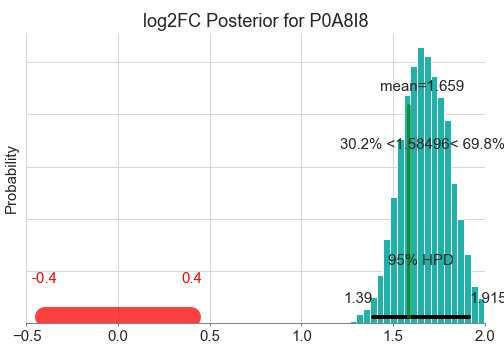
\includegraphics[width=\linewidth]{traceplots/P0A8I8_seq.png}
\end{subfigure}
\bigskip
\begin{subfigure}{\textwidth}
\centering
\caption*{B}
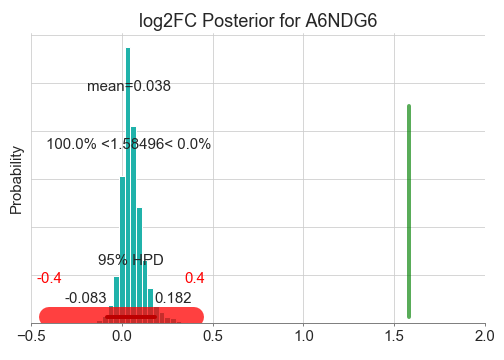
\includegraphics[width=\linewidth]{traceplots/A6NDG6_seq.png}
\end{subfigure}
\caption[Traceplot from sequence modelling of peptide effect]{Traceplot obtained after fitting the extended model on the test proteins mentioned in \ref{subsec:basic_model}. No feature was found to have any predictive power.}
\label{fig:traceplots_seq}
\end{figure}

\section{Discussion}

A list of points to address to improve how BayesQuant works is discussed in this section.

\subsection{Improving usability: parallelization}

While BayesQuant performed well on the majority of proteins, it took around 30 seconds to approximate each protein\textquotesingle s posterior distributions using \ac{VI}, and more than two minutes with \ac{MCMC} methods. This translates to a dataset of 1k proteins taking 500 minutes (>8h) to be processed. However, the average modern computer comes with several processors that could support the parallelization of the program in several threads, decreasing the total computing time.

\subsection{Further robustness and validation checks}

A solid way of checking the results are not flawed is the specification of alternative priors. Unless precise prior knowledge is available, the selection of one prior over another to model the beliefs about the system should not have great impact on the results. It is for that reason that models built upon different priors could be run to further validate the program. Moreover, a formal posterior validation beyond visual inspection of simulated data could be implemented.


\subsection{Advanced model comparison}

Likewise, a formal way of establishing the \ac{ROPE} in the quantification context could be enacted depending on the data. On the other hand, a more advanced model comparison method could be built upon the Bayes factor. The Bayes factor is defined as the ratio of the posterior probability of two models given the data \cite{Kruschke}. It could be used to measure how much more likely a model taking into account a treatment effect is compared to another one where the treatment effect is considered null i.e the \ac{log2FC} is set to 0. The result would provide an alternative criterion for the declaration of a protein being differentially abundant.

\subsection{Sequence-based modelling of the peptide effect}

Unfortunately, during the development of the project, it was acknowledged that the peptide effect is a very difficult phenomenon to capture in a simple Bayesian model as the one presented in this work. This is due to the motley and multilevel nature of the noise caused by the aminoacidic sequences:

\begin{itemize}

\item The protein neighborhood, which might affect the protease\textquotesingle s efficiency.

\item The competitive ionization problem, introduced in chapter \ref{chap:mass_spec} (\ref{subsec:the_ion_source}) implies that ionization prediction cannot be achieved without models that do not replicate this process mathematically. Thus, the ionization of a peptide ought to be predicted taking into account the peptide mix with which it accessed the ion source as a whole.

%which states that the ionization efficiency of a peptide will not just depend of its sequence, but also of that of its competitors in the ion source. This is due to the ion source providing a limited amount of charges for an excess peptide input. Therefore, a different number of instances of the same peptide acquire charge, depending on how efficient the other peptides simultaneously present are.

\item The mobile proton model \cite{Boyd2010}, which states that the peptide\textquotesingle s fragmentation pattern changes drastically depending on the number of charges and its distribution on the sequence. The charge distribution is hypothesised to be in turn determined by the position of positive residues that can allocate the charges. This phenomenon implies that the \ac{PSM} step is more difficult as a different spectrum is expected for molecules with the same peptide sequence but different charges. The decreased identifications and quality of the peaks worsen the performance of feature extraction algorithms like the Apex module in moFF. In turn, this results in the injection of more noise in the quantification data.

\item The characterization of powerful sequence properties that specifically capture differential ionization efficiency is undone work, as most feature extractors are designed to solve different problems, like protein structure prediction.

\end{itemize}

Modelling such a complex phenomenon will require accordingly complex predictive architectures and the introduction of proper neural networks, capable of deciphering the intricate pattern mapping sequence to noise in the spectrometer\textquotesingle s measurements. The development of very new RAW spectra-files parsing-tools like RawQuant \cite{Kovalchik2018} could be used in a future implementation to provide the required feature-rich data.


\subsection{Posterior assessment of the effects}

The characterization of the uncertainty behind a \ac{log2FC} estimate can be used to better inform downstream analysis programs and eventually help interpret the biological results. For example, a functional analysis program could decide to drop proteins declared differentially abundant if the uncertainty is greater than a threshold. A Gene Set Enrichment Analysis (\ac{GSEA}) could make use of the probabilistic information to refine its results.

Moreover, the estimation of the different run effects could be used to help \ac{MS} technicians assess the presence of batch effects in their experiments, and correct them in future analyses.

\section{Conclusion}

A Bayesian framework for the relative quantification of protein abundance ratios (Fold-Change, FC) using \ac{MS1} intensity was presented in this chapter. Unlike the currently prevailing methods in the field, it gives uncertainty estimates that provide a direct interpretation about the accuracy of the quantification. Moreover, preliminary results on the sequence modelling of the peptide bias revealed that more complex architectures and sequence features are required to model noise with peptide sequences. Finally, the method can be used to investigate the presence of batch effects in \ac{MS} experiments for their minimisation in future experiments. While the software can be integrated in any pipeline producing peptide-level data, further testing and improvements are probably required for optimal performance.

\chapter{Pipeline benchmarking on \ac{NZ} data}
\label{chap:benchmark}

\section*{Summary}

A second benchmark dataset was run through the programmes presented in chapters \ref{chap:pipeline} and \ref{chap:model} to showcase their performance. The experimental design attempted to capture a protein profile change reflecting a known biological process. Thus, a successful computational analysis of the dataset should reflect the same phenomenon. The results confirmed that the computational analysis successfully captured this response. It was concluded that the software can be used in future experiments where the biological phenomena underlying the data are not known.

\section{Introduction}

The protein ratios across conditions are not known in ordinary datasets. In order to judge the resolving power of the mass spectrometry and shotgun proteomics workflows presented in this work, an in-house dataset attempting to capture an immunological response was generated. Therefore, even though true protein ratios were not known \textit{a priori}, the analysis should find proteins related to the immunological response to be significantly differentially abundant. 

Moreover, a function inference step from the estimated protein \ac{log2FC} values is required to arrive to biological interpretations like that. These kind of analysis is common to all omics (genomics, transcriptomics, ...) and can be completed with Gene Set Enrichment Analysis \ac{GSEA} and Pathway Analysis, among others.

\subsection{Goals}

\begin{enumerate}

\item Gauge the analytical power of the computational analyses explained in the previous chapters.

%\item Compare its results with the commercial software currently in use.

\item Propose a biological inference pipeline to complete the proteomics workflow.

\end{enumerate}


\section{Materials and Methods}

\subsection{Sample preparation}

THP-1 cells were grown in RPMI1640 (Sigma) supplemented with 10\% FBS (SeraLab) and 1\% pen/strep (Gibco). Stimulation of THP-1 cells was done in 48-well plates (Gibco) with $2 \times 10^6$ cells/well. Cells were exposed to 500 ng/mL LPS (E. coli O111:B4) (+LPS) or nothing (-LPS) for 48 hours in 37 degrees, 5\% \ce{{CO}_2}. After stimulation supernatants were collected and cell pellets were washed in PBS (Gibco). Both supernatants and pellets were frozen (-20 degrees). This work was carried out by Esben G. W. Schmidt. Only the pellet samples were considered for the analysis. 
 
\subsection{Mass Spectrometry analysis}

Peptide digest of THP-1 samples were prepared using a filter assisted sample preparation protocol (FASP). Online desalting and nanoscale LC separation of tryptic peptides was performed with an Dionex Ultimate 3000 Dual –column nano-liquid chromatography system (Thermo Scientific) equipped with two Acclaim PepMap nano-trap columns, 20 mm, 75µ I.D., 3µ particles and two analytical Acclaim PepMap C18, 150 mm, 75µ capillary columns with 2µ particles (Thermo Scientific). Mobile phase A was 0.1\% formic acid (FA) in water and mobile phase B was 0.1\% FA in acetonitrile. Peptides were separated using a 60 min gradient from 5\% to 30\% mobile phase B at 350 nl/min and 35°C injecting samples on the two analytical columns in sequential randomized design. Eluting peptides were analyzed using data-dependent acquisition on an LTQ-Orbitrap Velos Pro mass spectrometer (Thermo Scientific). Each MS scan (400-1600 m/z) was acquired at a resolution of 30000 FWHM followed by 10 low resolution LTQ MS/MS scans triggered above an intensity of 10000 using collision induced dissociation CID (normalized collision energy 35). This work was carried out by David Gleerup and Anders M. B. Giessing.


%In short the FASP method is a filter aided in-solution sample preparation technique comprising of protein extraction with strong chaotropic reagents such as urea or Guanidine-HCL, protein precipitation with TCA, and digestion using trypsin under denaturing conditions of reduced and alkylated protein.  Tryptic peptides are extracted from the filter and analyzed by LC/MS. 


%Acquired MS data was processed and annotated using Genedata Expressionist. Acquired MS/MS spectra were searched against Homo sapiens reference proteome database taken using an in-house Mascot server ver. 2.5.1 (Matrix Science). Searches were conducted as follows: semi-tryptic specificity allowing up to two missed cleavages, 10 ppm peptide and 0.6 Da fragment ion tolerances, with carboiodimethyl of cysteine as fixed modification as well as variable modifications consisting of oxidation of methionine and deamidation (NQ). The final protein list was compiled when 2 or more unique peptides per protein were identified with a with a false Discovery Rate (FDR) cutoff of 1%, estimated using a target-decoy search strategy.  



\subsection{Computational analysis}

The resulting .RAW files were processed with the two different pipelines introduced in the present work. (I) Compomics+MSqRob and (II) Compomics+BQ (Compomics and BayesQuant). The search settings were identical to those used in chapter \ref{chap:pipeline}, except for the proteome databases employed, which consisted of \textit{Homo sapiens} only. The validation filters, \ac{MBR}, MS1 Apex intensity, and MSqRob preprocessing parameters were also set to those used previously, for simplicity. The two pipelines used thus diverged only in the quantification engine, being identical in all previous steps.

In the Compomics+MSqRob pipeline, a protein was declared to be differentially abundant (\ac{DAP}) between the 2 conditions assayed if the result of the student\textquotesingle s-T test implemented in MSqRob returned a q-value less than 0.05. The criteria in the Compomics+BayesQuant pipeline was the absence of overlap between the \ac{ROPE} [-0.4, 0.4] and the 95\% \ac{HPDI}.


\subsection{Biological inference}

The gProfiler R package \cite{Boyd2010} was used to perform \ac{GSEA}, and its results were visualized with the REVIGO tool \cite{Supek2011}.

Pathways analysis was executed with the ComPath Webserver \cite{Domingo2018}. UniprotKB IDs were transformed to "Gene name" IDs, as required by the tool, using the Retrieve/ID mapping tool from Uniprot. The KEGG \cite{Kanehisa2000} and Reactome \cite{Croft2014} databases were used as source.

Protein interactions were explored by querying the STRING database \cite{Szklarczyk2017} with the list of \ac{DAP}s produced by MSqRob.
 
\section{Results}

\subsection{Compomics+MSqRob}

Data on 6444 peptides, as collected in the peptide summary file from moFF, was passed to MSqRob, resulting in the quantification of 1433 proteins. A histogram of the \ac{log2FC} reveals that in most cases, not enough evidence was collected to declare the \ac{log2FC} different from 0 (see figure \ref{fig:compomics_rob} A). Remarkably, the distribution was shifted toward negative values, depicting that most of the proteins for which a non-null estimate was provided were more abundant in the +LPS condition. A volcano plot (see figure \ref{fig:compomics_rob} B), reveals that the majority of the 49 protein groups passing the significance criteria ($q-value < 0.05$), displayed an absolute value of the \ac{log2FC} less than 1. However, all were considered differentially abundant. The 32 protein groups composed by a single protein (single protein \ac{DAP}s) are shown in table \ref{tab:thp1_rob_results}.

% latex table generated in R 3.4.4 by xtable 1.8-2 package
% Sat Jul 21 16:02:33 2018
\begin{table}[!h]
\centering
\begin{tabular}{rllrr}
  \hline
 & Protein & Name & log2FC & qval \\ 
  \hline
  1 & P02792 & Ferritin light chain & 9.03E-01 & 2.32E-04 \\ 
  2 & Q04760 & Lactoylglutathione lyase & -7.24E-01 & 2.32E-04 \\ 
  3 & P13796 & Plastin-2 & -6.54E-01 & 2.32E-04 \\ 
  4 & P28066 & Proteasome subunit alpha type-5 & -6.88E-01 & 8.24E-04 \\ 
  5 & P09874 & Poly [ADP-ribose] polymerase 1 & -3.68E-01 & 2.48E-03 \\ 
  6 & P53396 & ATP-citrate synthase & -3.79E-01 & 3.25E-03 \\ 
  7 & P50552 & Vasodilator-stimulated phosphoprotein & -6.95E-01 & 1.43E-02 \\ 
  8 & P54577 & Tyrosine--tRNA ligase, cytoplasmic & -4.21E-01 & 2.71E-02 \\ 
  9 & Q15393 & Splicing factor 3B subunit 3 & -1.18E+00 & 2.88E-02 \\ 
  10 & P08567 & Pleckstrin & -1.26E+00 & 2.96E-02 \\ 
  11 & P50990 & T-complex protein 1 subunit theta & -3.60E-01 & 2.96E-02 \\ 
  12 & Q7RTV0 & PHD finger-like domain-containing protein 5A & -1.26E+00 & 2.96E-02 \\ 
  13 & O75083 & WD repeat-containing protein 1 & -6.55E-01 & 3.12E-02 \\ 
  14 & P17812 & CTP synthase 1 & -4.60E-01 & 3.12E-02 \\ 
  15 & Q14498 & RNA-binding protein 39 & -1.50E+00 & 3.29E-02 \\ 
  16 & P60903 & Protein S100-A10 & 1.13E+00 & 3.29E-02 \\ 
  17 & P26038 & Moesin & -3.91E-01 & 3.37E-02 \\ 
  18 & O75368 & SH3 domain-binding glutamic acid-rich-like p & -6.15E-01 & 3.37E-02 \\ 
  19 & Q8TEM1 & Nuclear pore membrane glycoprotein 210 & -8.24E-01 & 3.54E-02 \\ 
  20 & Q01518 & Adenylyl cyclase-associated protein 1 & -3.51E-01 & 3.54E-02 \\ 
  21 & Q08211 & ATP-dependent RNA helicase A & -4.19E-01 & 3.54E-02 \\ 
  22 & Q14566 & DNA replication licensing factor MCM6 & -4.33E-01 & 3.68E-02 \\ 
  23 & P30086 & Phosphatidylethanolamine-binding protein 1 & -6.31E-01 & 3.68E-02 \\ 
  24 & O43143 & RNA helicase DHX15 & -1.30E+00 & 3.80E-02 \\ 
  25 & O75691 & SMPC 20 homolog & -1.26E+00 & 3.80E-02 \\ 
  26 & P27797 & Calreticulin & -4.63E-01 & 3.80E-02 \\ 
  27 & P41218 & Myeloid cell nuclear differentiation antigen & -4.49E-01 & 3.80E-02 \\ 
  28 & Q15056 & Eukaryotic translation initiation factor 4H & -3.62E+00 & 3.98E-02 \\ 
  29 & P04406 & Glyceraldehyde-3-phosphate dehydrogenase & -1.90E+00 & 3.98E-02 \\ 
  30 & P00492 & Hypoxanthine-guanine phosphoribosyltransferase & -4.54E-01 & 4.12E-02 \\ 
  31 & P50440 & Glycine amidinotransferase, mitochondrial & -1.02E+00 & 4.50E-02 \\ 
  32 & P62857 & 40S ribosomal protein S28 & -5.50E-01 & 4.98E-02 \\ 
   \hline
\end{tabular}
\caption{THP-1 MSqRob results. 32 single-protein groups were found to be differentially abundant under significance criteria of q-value less than 0.05. The protein id, the gene name, the point estimate of its \ac{log2FC} and its significance is shown}
\label{tab:thp1_rob_results}
\end{table}


\begin{figure}[!h]
\begin{subfigure}{0.45\textwidth}
\centering
\caption*{A}
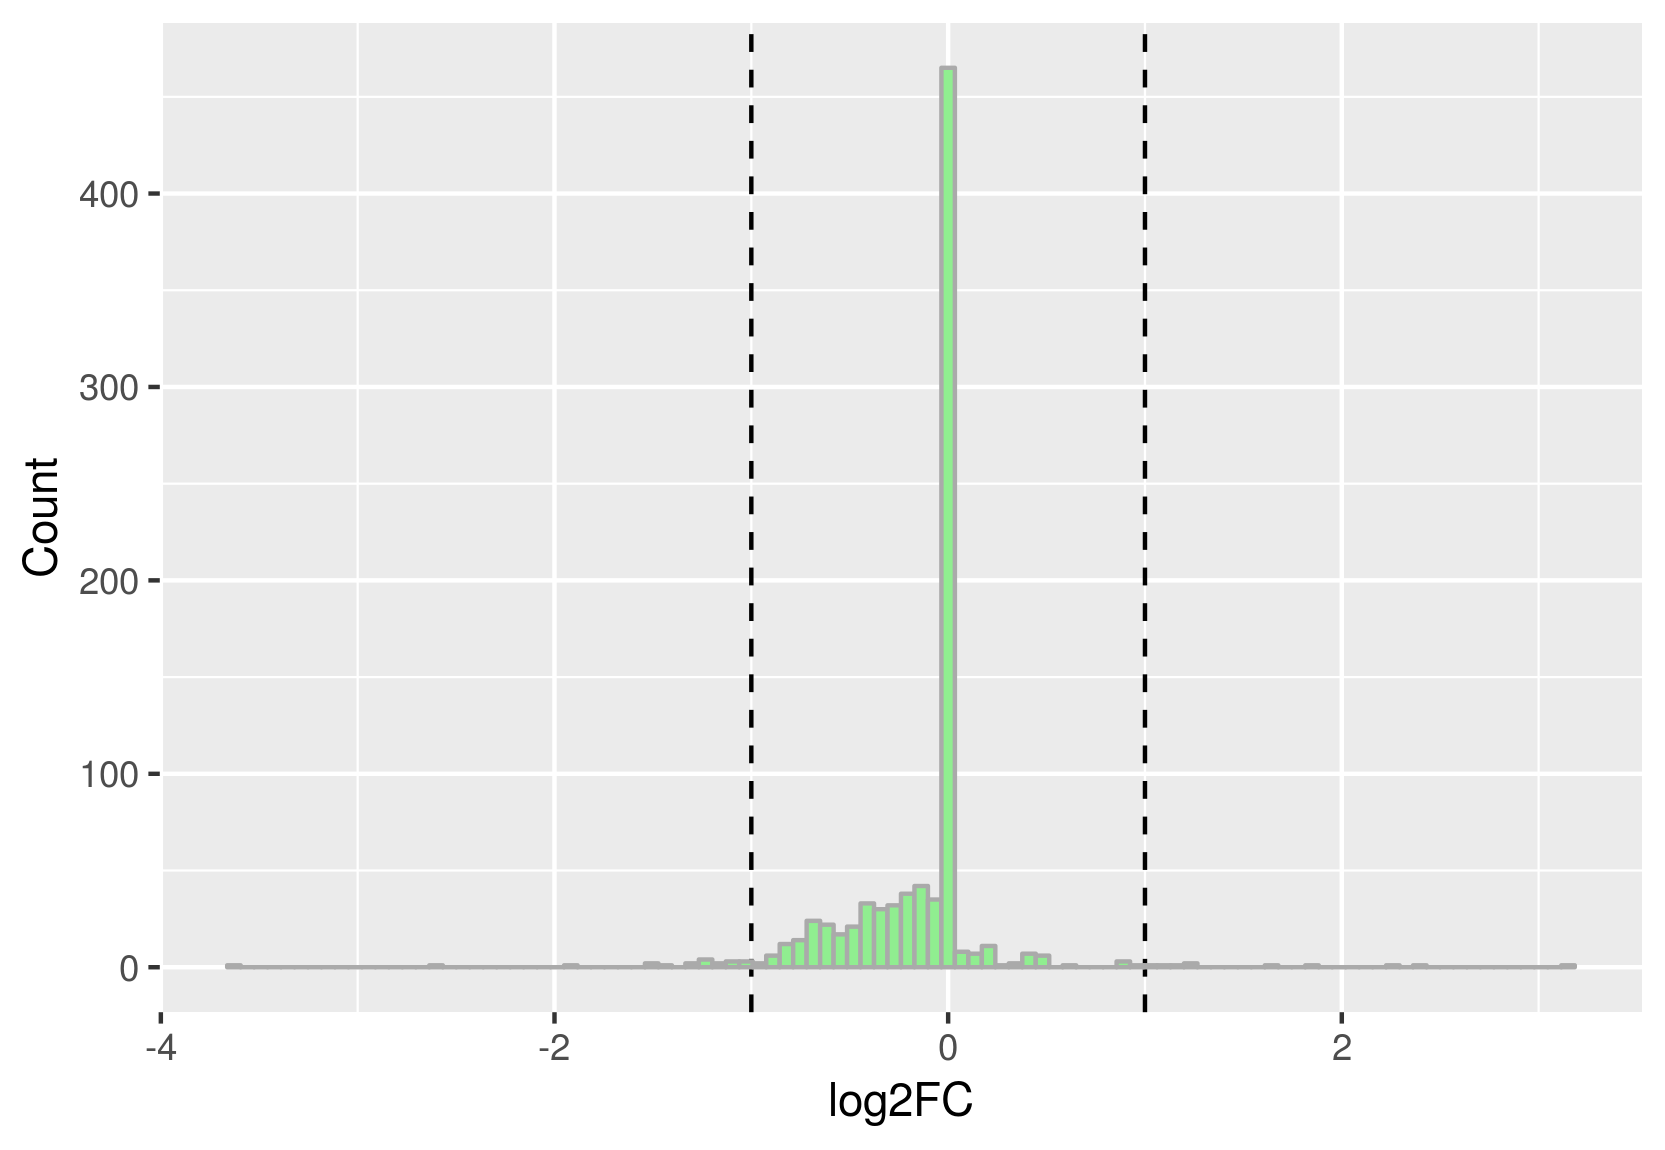
\includegraphics[width=.9\linewidth]{histogram_msqrob}
\end{subfigure}
\begin{subfigure}{0.45\textwidth}
\centering
\caption*{B}
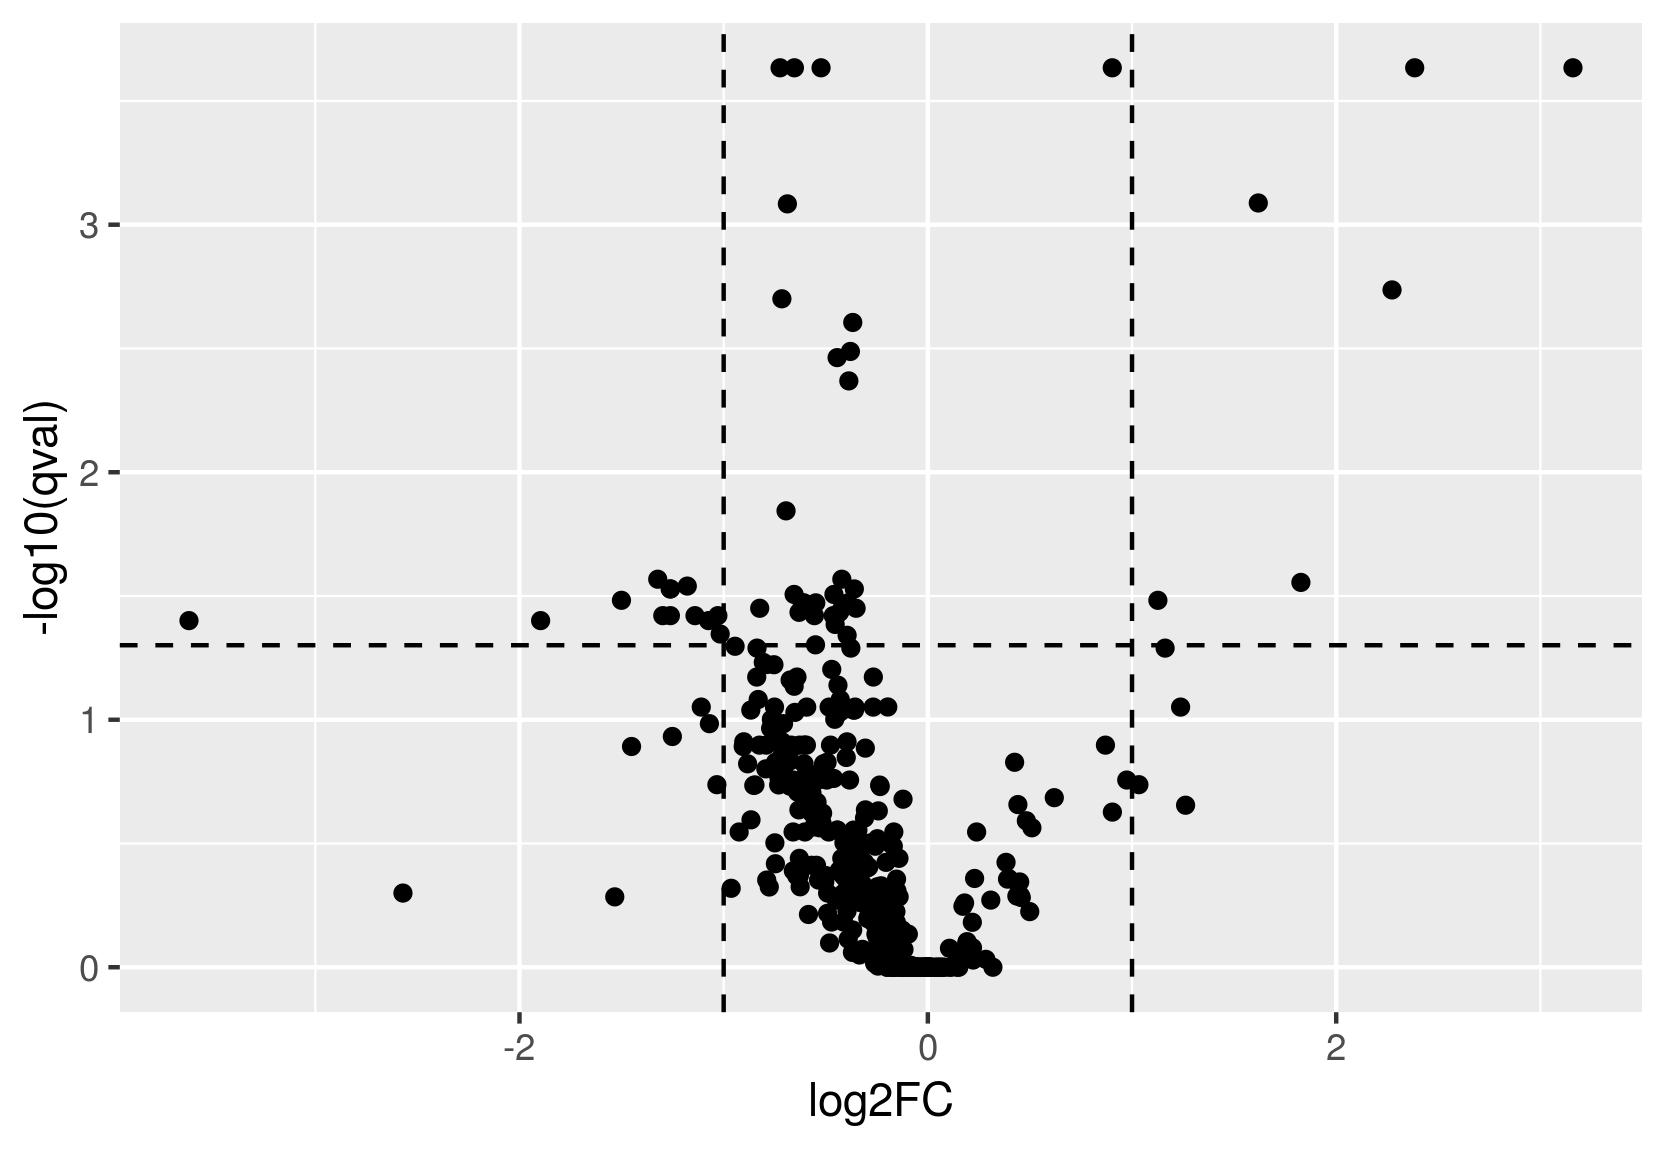
\includegraphics[width=.9\linewidth]{volcano_plot_msqrob}
\end{subfigure}
\caption[Compomics+MSqRob results on THP-1 dataset]{\textbf{Compomics+MSqRob results}. \textbf{A} Histogram of the estimated \ac{log2FC}. \textbf{B} Volcano plot, showing the point estimate of the \ac{log2FC} on the x axis, and the minus logarithm of the p-value on the y-axis.}
\label{fig:compomics_rob}
\end{figure}



\subsection{Compomics+BayesQuant}

After preprocessing and missing-data handling, a dataset of 1641 peptides was passed to BayesQuant, and 269 proteins were quantified. A histogram of the mean of the inferred posterior distributions manifests its centrality, with most values within the predefined \ac{ROPE} of [-0.4, 0.4]. In line with what was observed in the results above, the distribution was found to be skewed toward negative values (see figure \ref{fig:compomics_bq}A). Only four proteins were assigned a 95\% \ac{HPDI} not touching the \ac{ROPE} (see figure \ref{fig:compomics_bq}B and table \ref{tab:thp1_bq_results}). The distribution of the \ac{HPDI} width summarises the overall uncertainty in the estimation process. Most proteins had a very narrow HPDI, as shown in figure \ref{fig:compomics_bq}C. As expected, the width of the interval exhibited some degree of correlation with the mean of the posterior, as shown in figure \ref{fig:compomics_bq}D.

% latex table generated in R 3.4.4 by xtable 1.8-2 package
% Sat Jul 21 18:02:39 2018
\begin{table}[!h]
\centering
\begin{tabular}{rlrrrr}
  \hline
 & Protein & log2FC & HPDI start & HPDI end & Peptides \\ 
  \hline
& O75475 & -0.61 & -0.80 & -0.43 & 2 \\ 
   & O15144 & -0.75 & -0.98 & -0.51 & 3 \\ 
   & P02792 & 0.50 & 0.41 & 0.58 & 4 \\ 
   & P04406 & -1.09 & -1.45 & -0.77 & 4 \\ 
   \hline
\end{tabular}
\caption{\ac{DAP}s declared by the Compomics+BayesQuant pipeline.}
\label{tab:thp1_bq_results}
\end{table}


\begin{figure}[H]
\centering
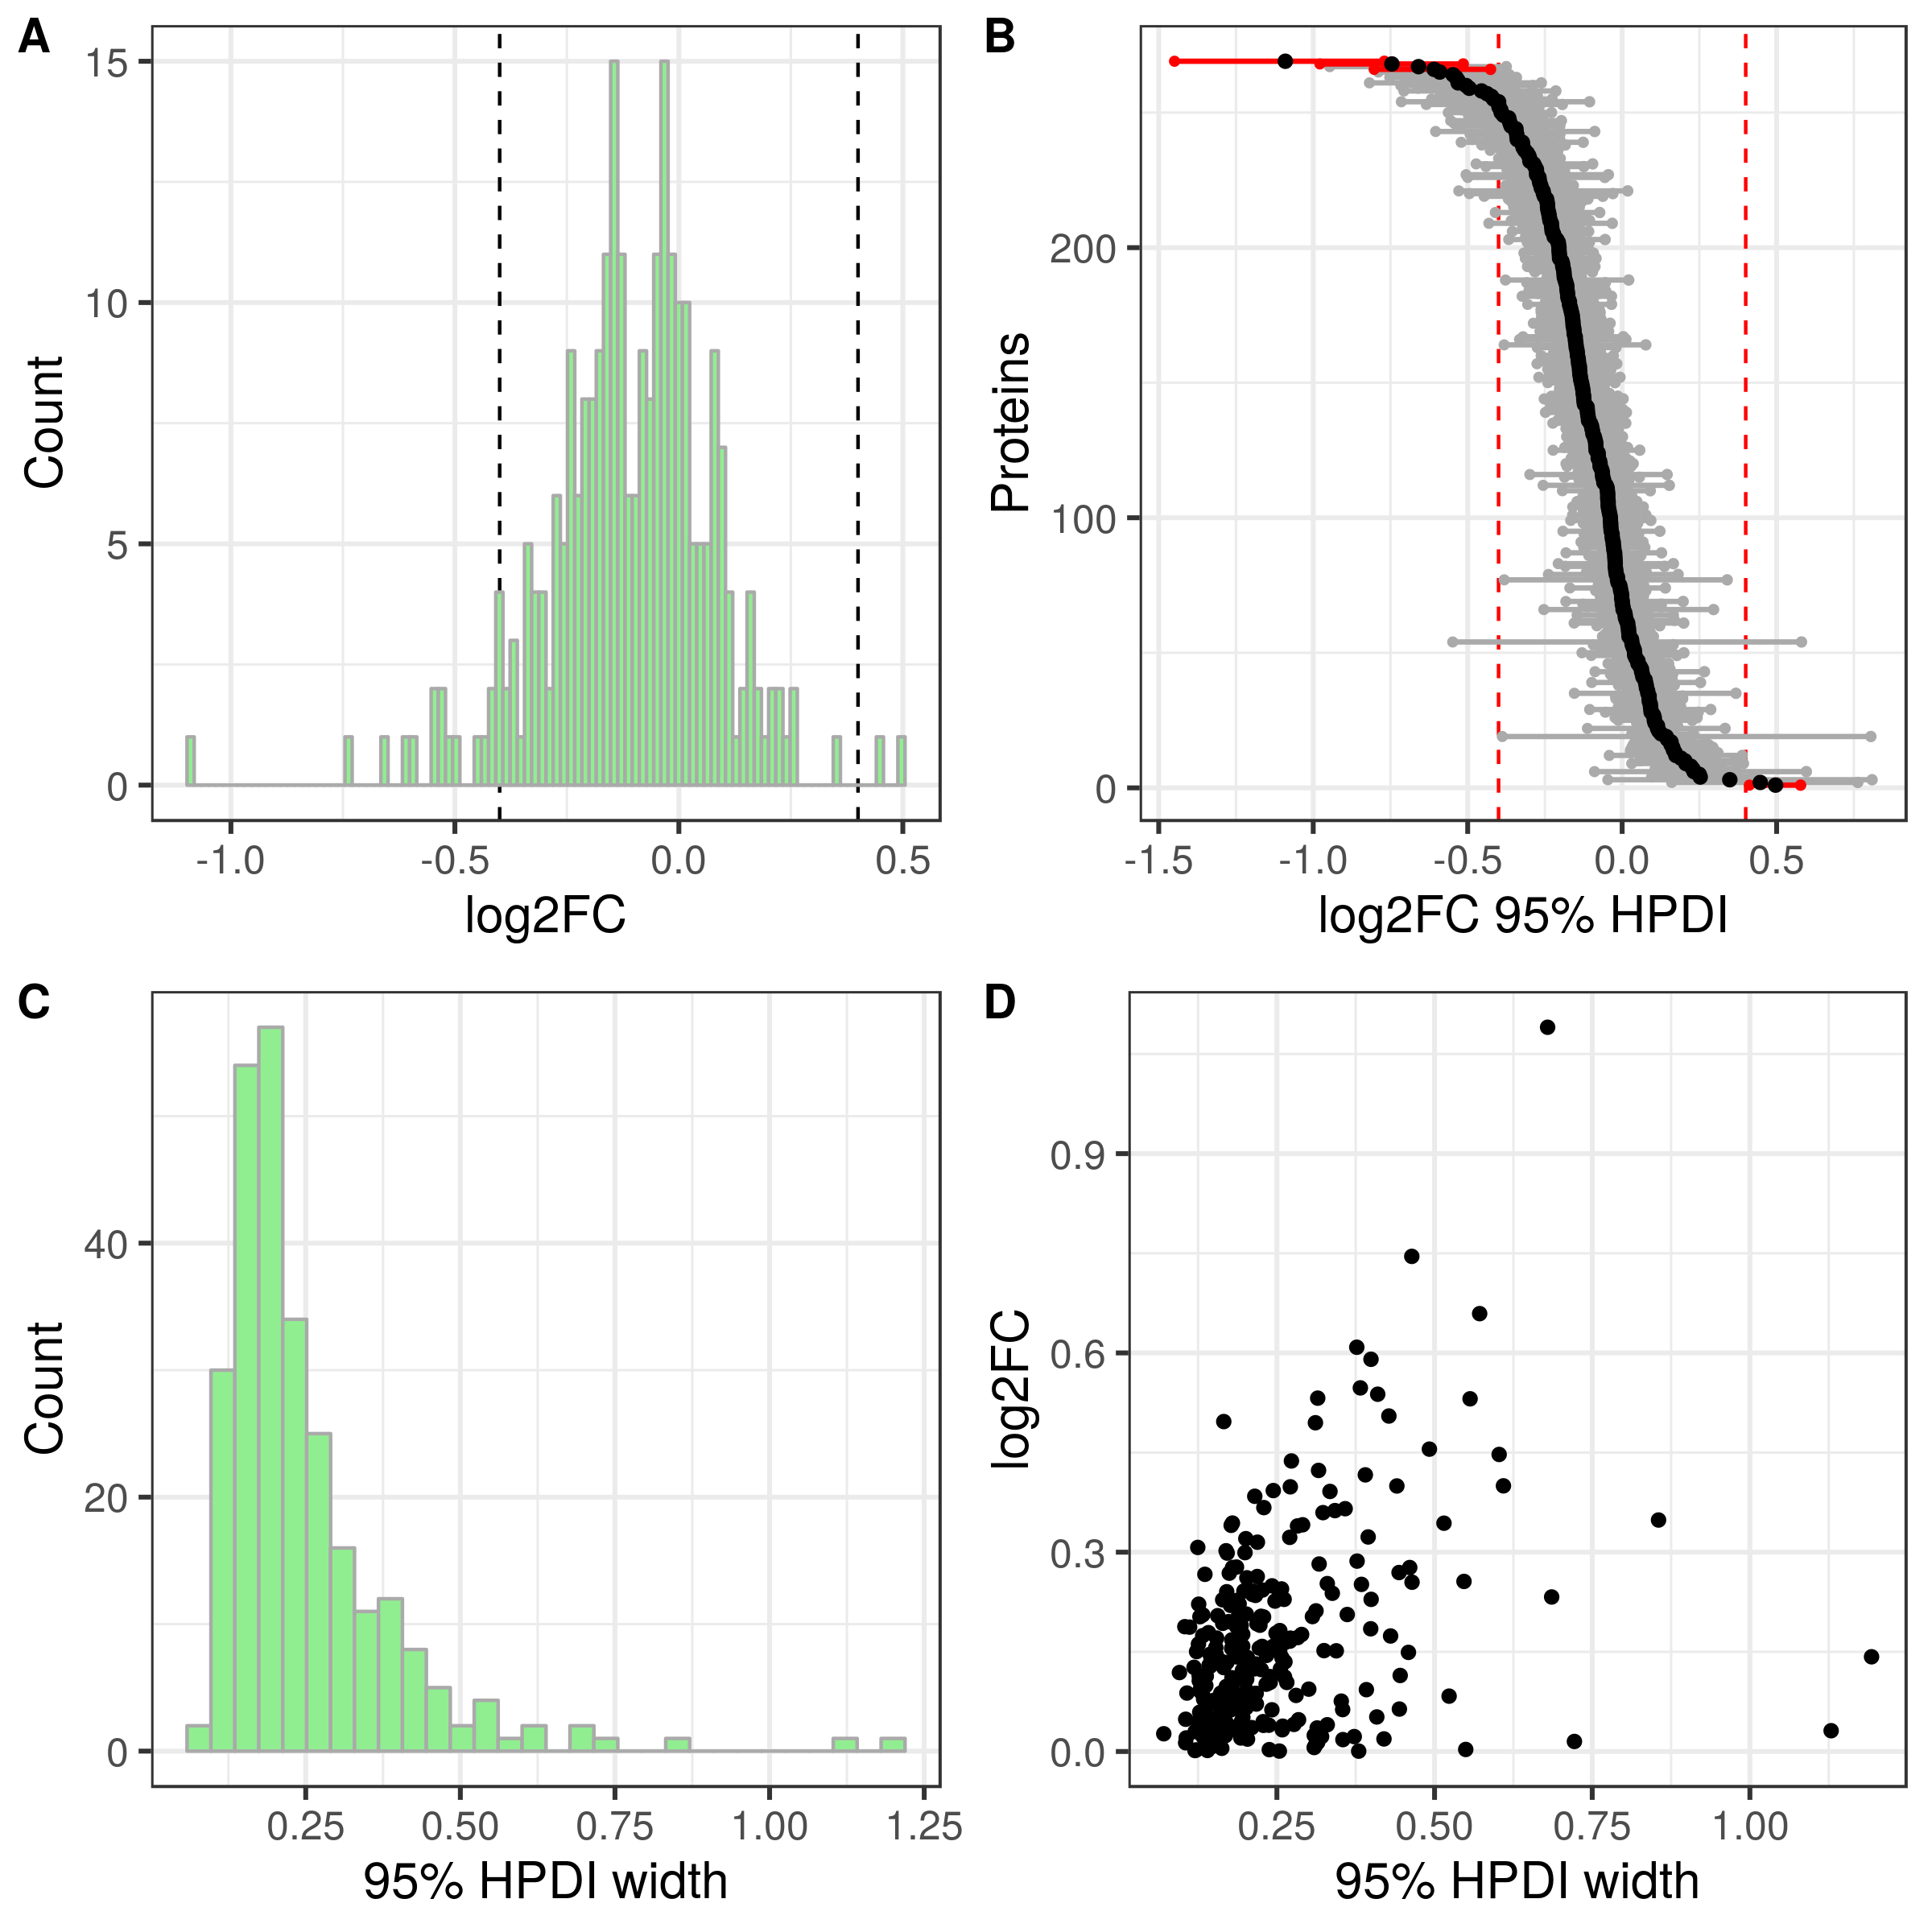
\includegraphics[width=\linewidth]{bq_comb_bq}
\caption[Compomics+BayesQuant results on the THP-1 dataset]{\textbf{BayesQuant results}. \textbf{A} Histogram of the mean of the posterior distributions. \textbf{B} Dumbbell plot, representing the 95\% \ac{HPDI} for all proteins. Black dots represent the mean, and intervals not overlapping the \ac{ROPE} are shown red. \textbf{C} Histogram of the 95\% \ac{HPDI} width, which can be used as proxy for the overall uncertainty in the quantified data. \textbf{D} Scatter plot of the 95\% \ac{HPDI} width and the  posterior \ac{log2FC} mean.}
\label{fig:compomics_bq}
\end{figure}


Given the scarcity of the results, it was decided to continue the analyses with MSqRob output only.

\subsection{Functional analysis}

A \ac{GSEA} performed on the list of 32 single-protein \ac{DAP}s produced by MSqRob (see table \ref{tab:thp1_rob_results}) illustrates the most over-represented biological processes, cellular compartments and molecular functions, compared to the human background. The 20 most significant terms found in the dataset are displayed in table \ref{tab:gsea}.


% latex table generated in R 3.4.4 by xtable 1.8-2 package
% Sat Jul 21 19:00:27 2018
\small
\begin{table}[!h]
\centering
% latex table generated in R 3.4.4 by xtable 1.8-2 package
% Sun Jul 22 12:29:16 2018
\begin{tabular}{rllrrrl}
  \hline
 & Term ID & Term Name & Query & Term & Ov & P-value \\ 
  \hline
1 & GO:0070062 & extracellular exosome &  32 & 2774 &  19 & 1.17e-05 \\ 
  2 & GO:1903561 & extracellular vesicle &  32 & 2793 &  19 & 1.31e-05 \\ 
  3 & GO:0043230 & extracellular organelle &  32 & 2795 &  19 & 1.33e-05 \\ 
  4 & GO:0005615 & extracellular space &  32 & 3958 &  20 & 6.76e-04 \\ 
  5 & GO:0035578 & azurophil granule lumen &  32 &  90 &   5 & 8.87e-04 \\ 
  6 & GO:0044421 & extracellular region part &  32 & 4119 &  20 & 1.34e-03 \\ 
  7 & GO:0002376 & immune system process &  32 & 2949 &  17 & 1.74e-03 \\ 
  8 & GO:0060205 & cytoplasmic vesicle lumen &  32 & 335 &   7 & 2.54e-03 \\ 
  9 & GO:0031983 & vesicle lumen &  32 & 336 &   7 & 2.59e-03 \\ 
  10 & GO:0005576 & extracellular region &  32 & 4925 &  21 & 4.95e-03 \\ 
  11 & GO:0003723 & RNA binding &  32 & 1787 &  13 & 5.50e-03 \\ 
  12 & GO:0065003 & protein-containing complex assembly &  32 & 1803 &  13 & 6.08e-03 \\ 
  13 & GO:0003725 & double-stranded RNA binding &  32 &  65 &   4 & 9.71e-03 \\ 
  14 & GO:0005766 & primary lysosome &  32 & 153 &   5 & 1.23e-02 \\ 
  15 & GO:0042582 & azurophil granule &  32 & 153 &   5 & 1.23e-02 \\ 
  16 & HPA:006020\_13 & caudate; neuronal cells &  14 & 311 &   5 & 1.35e-02 \\ 
  17 & GO:0031982 & vesicle &  32 & 4271 &  19 & 1.38e-02 \\ 
  18 & GO:1990904 & ribonucleoprotein complex &  32 & 836 &   9 & 1.44e-02 \\ 
  19 & GO:0001775 & cell activation &  32 & 1359 &  11 & 1.60e-02 \\ 
  20 & HPA:022020\_13 & hippocampus; neuronal cells &  14 & 331 &   5 & 1.81e-02 \\ 
   \hline
\end{tabular}

%\begin{tabular}{rllllll}
%  \hline
% & Term ID & Term Name & Query & Term & Ov & P-value \\ 
%  \hline
%1 & GO:0070062 & extracellular exosome &  32 & 2774 &  19 & 1.17e-05 \\ 
%  2 & GO:1903561 & extracellular vesicle &  32 & 2793 &  19 & 1.31e-05 \\ 
%  3 & GO:0043230 & extracellular organelle &  32 & 2795 &  19 & 1.33e-05 \\ 
%  4 & GO:0005615 & extracellular space &  32 & 3958 &  20 & 6.76e-04 \\ 
%  5 & GO:0035578 & azurophil granule lumen &  32 &  90 &   5 & 8.87e-04 \\ 
%  6 & GO:0044421 & extracellular region part &  32 & 4119 &  20 & 1.34e-03 \\ 
%  7 & GO:0002376 & immune system process &  32 & 2949 &  17 & 1.74e-03 \\ 
%  8 & GO:0060205 & cytoplasmic vesicle lumen &  32 & 335 &   7 & 2.54e-03 \\ 
%  9 & GO:0031983 & vesicle lumen &  32 & 336 &   7 & 2.59e-03 \\ 
%  10 & GO:0005576 & extracellular region &  32 & 4925 &  21 & 4.95e-03 \\ 
%  11 & GO:0003723 & RNA binding &  32 & 1787 &  13 & 5.50e-03 \\ 
%  12 & GO:0065003 & Complex assembly &  32 & 1803 &  13 & 6.08e-03 \\ 
%  13 & GO:0003725 & DS RNA binding &  32 &  65 &   4 & 9.71e-03 \\ 
%  14 & GO:0005766 & primary lysosome &  32 & 153 &   5 & 1.23e-02 \\ 
%  15 & GO:0042582 & azurophil granule &  32 & 153 &   5 & 1.23e-02 \\ 
%  16 & HPA:006020\_13 & caudate; neuronal cells &  14 & 311 &   5 & 1.35e-02 \\ 
%  17 & GO:0031982 & vesicle &  32 & 4271 &  19 & 1.38e-02 \\ 
%  18 & GO:1990904 & ribonucleoprotein complex &  32 & 836 &   9 & 1.44e-02 \\ 
%  19 & GO:0001775 & cell activation &  32 & 1359 &  11 & 1.60e-02 \\ 
%  20 & HPA:022020\_13 & hippocampus; neuronal cells &  14 & 331 &   5 & 1.81e-02 \\ 
%   \hline
%\end{tabular}
\caption{\ac{GSEA} results. The 20 most significant terms are displayed. The columns \textit{Query}, \textit{Term} and \textit{Ov} indicate the size of the query, the number of proteins under the term, and the overlap between them. The size of the query differs in the GO and HPA terms repositories due to nomenclature mismatches.}
\label{tab:gsea}
\end{table}
\normalsize

On the one hand, nine terms (1, 2, 3, 4, 6, 8, 9, 10 and 17) were cell compartment terms associated with cellular secretion and the extracelullar space. On the other hand, five terms (5, 7, 14, 15, 19) were related to the immunological response. The remaining terms were connected to RNA functions.

These results can be better visualized by making use of a treemap (see figure \ref{fig:treemap}), which makes the interpretation of table \ref{tab:gsea} more straightforward.

\begin{figure}[!h]
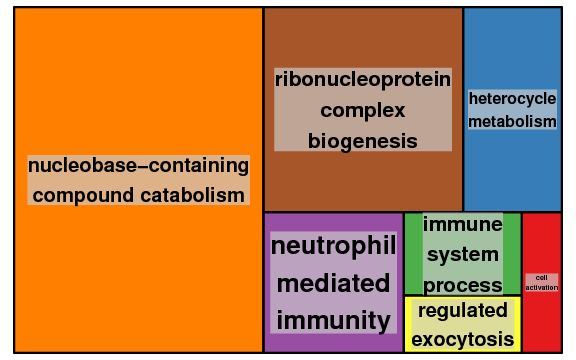
\includegraphics[width=\textwidth]{revigo_treemap.png}
\caption[REVIGO treemap]{\textbf{REVIGO treemap}. A top-level representation of the enriched GO-terms. Each top-level term is mapped to an area whose size is proportional to the significance of the term. This way, a big area indicates more enrichment \cite{Supek2011}.}
\label{fig:treemap}
\end{figure}

\subsection{Pathway analysis}

The UniprotKB to Gene name mapping of the set of 49 \ac{DAP}s (including multi-protein groups) returned by MSqRob produced a list of 51 entities. The list was supplied to the ComPath Pathway Enrichment tool to highlight which cellular pathways were over-represented compared to the human background. 50 entities were mapped to the database. In agreement with the \ac{GSEA} results, a handful of pathways linked to the immune response were found to be significantly enriched (see table \ref{tab:pathway_enrichment}) (I) Immune System, (II) Innate Immune System, (III) Necroptosis (IV) Programmed Cell Death, (V) Regulation of Apoptosis, (VI) Leukocyte transedothelial migration. Moreover, the finding of several RNA related pathways exposed the presence of potential cell reprogramming, essential in any change in protein profile.

% latex table generated in R 3.4.4 by xtable 1.8-2 package
% Sat Jul 21 19:49:28 2018
\begin{table}[ht]
\centering
\begin{tabular}{rllrrl}
  \hline
 & Pathway & q-val & Ov & Size & DB \\ 
  \hline
1 & Neutrophil degranulation & 0.00e+00 &   9 & 479 & reactome \\ 
  2 & Immune System & 0.00e+00 &  15 & 2050 & reactome \\ 
  3 & Innate Immune System & 0.00e+00 &  10 & 1109 & reactome \\ 
  4 & Metabolism of RNA & 0.00e+00 &  10 & 666 & reactome \\ 
  5 & Processing of Pre-mRNA & 2.00e-04 &   5 & 240 & reactome \\ 
  6 & mRNA Splicing & 1.10e-03 &   4 & 180 & reactome \\ 
  7 & mRNA Splicing & 1.20e-03 &   4 & 188 & reactome \\ 
  8 & Metabolic pathways & 1.60e-03 &   8 & 1282 & kegg \\ 
  9 & Carbon metabolism & 2.90e-03 &   3 & 116 & kegg \\ 
  10 & Spliceosome & 4.00e-03 &   3 & 134 & kegg \\ 
  11 & Pentose phosphate pathway & 4.20e-03 &   2 &  30 & kegg \\ 
  12 & Base excision repair & 4.90e-03 &   2 &  33 & kegg \\ 
  13 & Ribosome & 5.30e-03 &   3 & 153 & kegg \\ 
  14 & Necroptosis & 6.10e-03 &   3 & 162 & kegg \\ 
  15 & Apoptosis & 6.60e-03 &   3 & 168 & reactome \\ 
  16 & Programmed Cell Death & 6.90e-03 &   3 & 171 & reactome \\ 
  17 & Regulation of Apoptosis & 1.08e-02 &   2 &  53 & reactome \\ 
  18 & Aminoacyl-tRNA biosynthesis & 1.55e-02 &   2 &  66 & kegg \\ 
  19 & Glycolysis / Gluconeogenesis & 1.59e-02 &   2 &  68 & kegg \\ 
  20 & Leukocyte transendothelial migration & 2.96e-02 &   2 & 112 & kegg \\ 
   \hline
\end{tabular}
\caption{Pathway Enrichment results. 50 proteins were mapped to pathway databases and an enrichment was performed. The 10 most significant pathways found in Reactome and Kegg are shown arranged by decreasing significance. The columns \textit{Ov} and \textit{Size} indicate the number of proteins shared between pathway and query, and the number of proteins included in the pathway, respectively. The input was always 49 set to protein groups.}
\label{tab:pathway_enrichment}
\end{table}

\subsection{Protein interaction analysis}

The same list supplied to ComPath was searched in the STRING database \cite{Szklarczyk2017} to screen for protein-protein interactions in the list. The database returns a protein association network (see figure \ref{fig:STRING}), that helps interpreting the information contained in gene sets. 49/51 terms were mapped to the resource and 15 of them were found to be included in the "immune system process" set, placing this biological process as the third most enriched with an FDR of 0.0387. 27 genes belonged to the "cellular nitrogen compound metabolic process" (FDR 0.0128).

\begin{figure}[!h]
\centering
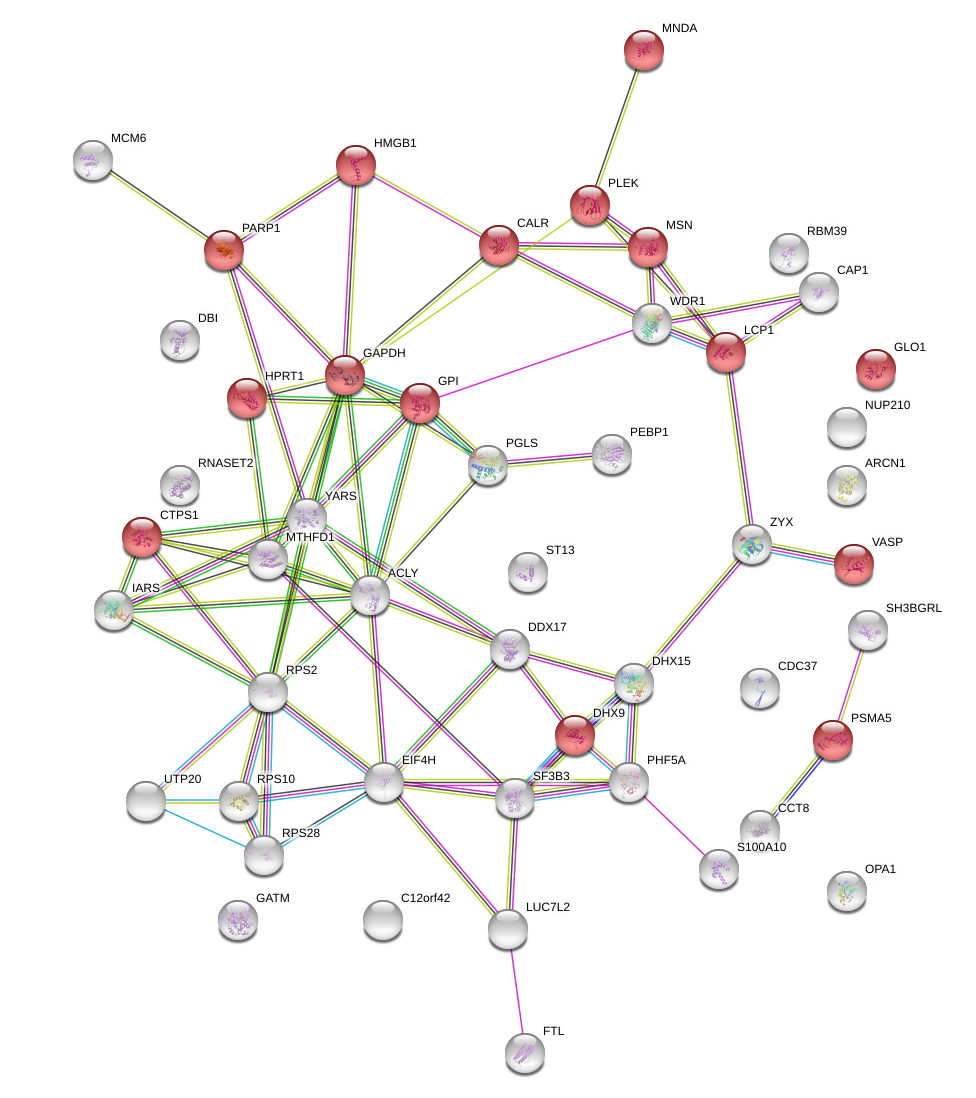
\includegraphics[width=\linewidth]{string_normal_image}
\caption[Protein interaction network]{\textbf{STRING interaction network}. Every node represents a protein in the list, and an edge between any pair represents evidence for some kind of association or interaction between them. Evidence is either experimentally determined or predicted using diverse methods. Red colored nodes are included in the "immune system process" set.}
\label{fig:STRING}
\end{figure}





\section{Discussion}

A discussion over the major issues and strengths detected while obtaining these results follows.


\subsection{Increasing the experiment data-throughput}

Six samples organized in two different treatments of three biological replicates without sample prefractionation each were analyzed. The resulting data throughput allowed for the performance of biological inference, as it successfully captured the undergoing biological processes. Nevertheless, more in-depth results would have been possible with (I) sample prefractionation, which improves peptide separation and allows for the collection and identification of more spectra \cite{Righetti2005}, and (II) the inclusion of technical replicates to differentiate the biological variability from experimental noise.

\subsection{Missing data handling}

One of the most frequent issues found when analyzing proteomics datasets is the handling of missing values \cite{Lazar2016}. The presence of missing data in many of the rows in the data passed to BayesQuant led to the dropping of 4803 out of 6443 peptides, producing a peptide dataset of only 1641 data points that accounted for 350 protein groups. Thanks to the missing data handling implemented in MSqRob, this tool quantified 1433 proteins, enough to continue the quantitative analysis (see table \ref{tab:balance}). However, the fact that the number of observed groups was 2787 implies that the management of missing values could potentially be improved in both tools, and particularly in BayesQuant.

\begin{table}[!h]
\centering
\begin{tabular}{|c|c|c|}
\hline 
Tool & Peptides & Proteins \\ 
\hline 
MSqRob & 6444 & 1433 \\ 
\hline 
BayesQuant & 1641 & 350 \\ 
\hline 
\end{tabular} 
\caption{Peptide input and quantified proteins for each tool in the THP1 dataset.}
\label{tab:balance}
\end{table}

Three different types of missing values have been defined \cite{Wei2018}:

\begin{enumerate}

\item Missing Completely At Random (MCAR): Unpredictable, caused by random errors in the data acquisition step and affecting the whole dataset.

\item Missing At Random (MAR): Caused by other observed variables. \textit{ Inaccurate peak detection and deconvolution of co-eluting compounds can be called MAR} \cite{Wei2018}.

\item Missing Not At Random (\ac{MNAR}): Caused by signals under the limit of detection (\ac{LOD}) of the spectrometer.

\end{enumerate}

While all three are relevant, \ac{MNAR} is particularly important because it introduces a bias in the dataset, where proteins are more likely to be quantified if their abundance is high enough in all samples for their peptide signals to be above the \ac{LOD}. Thus, proteins exhibiting abundances below the \ac{LOD} due to the experimental treatment are bound to generate peptide data featuring missing values that, if not handled properly, are discarded. Subsequently, \ac{DAP}s or in general proteins with variant abundance become less likely to be quantified, complicating the extraction of relevant protein sets.

Missing data should be imputed at the peptide level. The implementation of a module performing this task prior to quantification would  improve the accuracy and throughput of the quantification process. Several approaches have been proposed, some within a probabilistic framework \cite{Lazar2016}. For example, in cases of clear \ac{MNAR}, imputation could be based on an inferred global \ac{LOD}, so that missing values are replaced with it. Work on this line could potentially boost the performance of BayesQuant.


\subsection{Applicability for Novozymes data}

\ac{NZ} data is frequently confidential and cannot be uploaded to public servers like STRING. However, many of the databases consulted in this work can be built locally, thus removing the need of data leaving the company\textquotesingle s facilities.



\section{Conclusion}
A fine biological interpretation of the results depends on the original question that motivated the study, and thus this chapter did not focus on that, but instead showed how it can be started with the output of the tools presented in the previous chapters. The results indicated the tools can be deployed to perform computational analyses and biological inference on protein samples with open-source software with no cost for \ac{NZ}. However, the absence of proper missing data handling developed into the inability to quantify hundreds of proteins, signaling what are the next steps to improve the tools. 
\chapter{Conclusion of the Thesis}
\label{chap:conclusion}

The pipelines presented in chapter \ref{chap:pipeline} offer output-rich and easy to deploy cost-free pieces of software. All of them have pros and cons, and their combined usage was found to provide the best results, underlining the importance of the development of programs implementing open data formats exchangeable across tools. More functionalities can be added, including \textit{de novo} and \ac{PTM} search, fractioned samples and missing data management. BayesQuant, the probabilistic framework for relative quantification, presented in chapter \ref{chap:model}, can be passed a peptide level dataset and provide estimates of the uncertainty beyond frequentist \ac{log2FC} estimates. It can be customized to expand its currently implemented model. The lack of success in the attempt to model the peptide bias using the aminoacidic sequence reveals the complexity of its origin. Recently developed tools  could be applied in future work to extract a feature-rich representation of the collected spectra that could be used to model this phenomenon with a Deep Learning approach. The results from chapter \ref{chap:benchmark} manifest that \ac{NZ} can at the same time decrease computational costs and access the state of the art in proteomics research by making use of the latest open-source software. In summary, this work grants exciting opportunities for developing workflows in the field.






\printbibliography


\end{document}
%%  ==================================================================
%%  End document
